\documentclass[11pt,a4paper,spanish]{book}
\usepackage[a4paper,left=3cm,right=2cm,top=3cm,bottom=2cm]{geometry}
\usepackage[pdftex]{graphicx}
%\usepackage{graphicx}
\usepackage[T1]{fontenc}
\usepackage[latin1]{inputenc}
\usepackage[spanish]{babel}
\usepackage{natbib}

%\usepackage[colorlinks=true,linkcolor=black,citecolor = blue, urlcolor= blue, breaklinks=true, naturalnames=true]{hyperref}
\usepackage[colorlinks=true,linkcolor=black,citecolor = black, urlcolor= blue, breaklinks=true, naturalnames=true]{hyperref}
\usepackage{breakurl} 
\usepackage{url}
\usepackage{float}
%\usepackage{listings}
\usepackage{color}
\usepackage{amssymb}
\usepackage{amsthm}

\newcounter{contejemplos} %contador de ejemplos
\newcounter{contdefiniciones} %contador de definiciones
\newcounter{contproposiciones} %contador de proposiciones

\definecolor{colorejemplo}{rgb}{0.8,0.85,1} %color para fondo de ejemplos

%\newenvironment{ejemplo}[1]{\begin{flushleft}
%    \refstepcounter{contejemplos} \textbf{Ejemplo
%      \arabic{contejemplos}: }\emph{#1}\newline}{\end{flushleft}
%  \normalsize} %ambiente ejemplos

%\newenvironment{ejemplo}[1]{\begin{quote}
%   \refstepcounter{contejemplos} \textbf{Ejemplo
%      \arabic{contejemplos}: }\emph{#1}\newline}{\end{quote}
 % \normalsize} %ambiente ejemplos

\newtheorem{definition}{Definici\'on}[section]

\newtheorem{proposition}{Proposici\'on}[section]

\newtheorem{teorema}{Teorema}[section]

\newtheorem{corolario}{Corolario}[section]

\newtheorem{demo}{Demostraci\'on}[section]

%\theoremstyle{plain}
%\theorembodyfont{\normalfont}
\newtheorem{ejemplo}{Ejemplo}[section]


\begin{document}

\renewcommand{\tablename}{Tabla}
\renewcommand{\listtablename}{\'Indice de tablas}

%Empieza la numeracin en nmeros romanos
\frontmatter
% Incluimos la cartula
%Observaci�n: Si bien la p�gina del prefacio dice que sea empty, deber�a comenzar alli la numeraci�n. Se sugiere numeraci�n romana. Recomenzar la numeraci�n en el primer cap�tulo de la tesis  con numeraci�n ar�biga.

\titlepage

\begin{center}
\ \\
\ \\
\vspace{-1cm}
 

\ \\

\vspace{0.5cm}
{\Large{\bf \sc Universidad Nacional del Comahue}}\\

\ \\
{\Large { \sc Facultad de Inform�tica}}\\

\vspace{-2.5cm}
\mbox{\hspace{-1cm}
\includegraphics[width=2.5cm,height=2.5cm]{unc.png}\hspace{13cm} 
\includegraphics[width=2.5cm,height=2.5cm]{fai.png}}


\vspace{6cm}

{\Large {\bf\sc Tesis de Licenciado en Ciencias de la Computaci�n}}\\
\ \\
\ \\
{\LARGE {\bf Planificaci\'on Continua mediante PDDL}}\\
\vspace{3cm}


{\Large Germ�n Alejandro Braun}\\
\vspace{2cm}

{\Large Director: Mg. Gerardo Parra}\\
\ \\
%{\Large [Nombre del CoDirector]}\\

\vfill
{\Large {\sc Neuqu�n}\hspace{6cm}{\sc Argentina}}\\
\ \\

{\Large 2012}\\

\end{center}

\pagebreak




% Incluimos la pgina de prefacio.
\ \\
\ \\
\label{pagpref}
\noindent{\LARGE \sc Prefacio}\\
\ \\
\ \\

\ \\

\ \\
\ \\


Esta tesis es presentada como parte de los requisitos finales para
optar al grado acad\'emico de {\em Licenciado/a en Ciencias de la
Computaci�n}, otorgado por la Universidad Nacional del Comahue, y no
ha sido presentada previamente para la obtenci�n de otro t�tulo en
esta Universidad u otras. La misma es el resultado de la investigaci�n
llevada a cabo en el Departamento de Teor\'ia de la Computaci\'on, 
de la Facultad de Inform�tica, en el per�odo comprendido entre Septiembre
del 2011 y Agosto del 2012, bajo la direcci�n del Mg. Gerardo Parra.




\vspace{3cm}


\ \\
{\flushright Germ\'an Braun\\
{\sc Facultad de Inform�tica \\
Universidad Nacional del Comahue}\\
{\em Neuqu\'en, 6 de Septiembre de 2012.}\\}

\vfill

\begin{center}
%
\framebox{\begin{minipage}[t]{0.9\columnwidth}%
\begin{flushleft}

\includegraphics[scale=0.035]{unc.png}

\vspace{-2cm}
{\large \hspace{5cm}\sc universidad
nacional del comahue} \\
\par\end{flushleft}
\begin{center}
{\large \qquad{}}{ \hspace{2.5cm} Facultad de Inform�tica}
\par\end{center}

\vspace{1cm}

\indent \ \ \ \ \ \ \ \ \ \ \ La presente tesis ha sido aprobada el d�a ........................., mereciendo la \\
\indent \ \ \ \  \ \ \ \ \ calificaci�n de .............................

\medskip{}

\vspace{1cm}
\end{minipage}}
\end{center}

\pagebreak


% Incluimos la pgina de dedicatorias. Esta pgina es opcional.
% Si la pgina no quiere ser incluida anteponga el smbolo "%" al comienzo de la siguiente lnea
\ \\
\ \\
\label{pagdedic}
\noindent{\LARGE \sc Dedicatorias}\\
\ \\
\ \\

\ \\

\ \\
\ \\
\emph{A mi mam\'a y a mi pap\'a, a quienes debo mi educaci\'on.}\\

\vfill
\pagebreak



% Incluimos la pgina de agradecimientos. Esta pgina es opcional.
% Si la pgina no quiere ser incluida anteponga el smbolo "%" al comienzo de la siguiente lnea
\ \\
\ \\
\label{pagagrad}
\noindent{\LARGE \sc Agradecimientos}\\
\ \\
\ \\

\ \\

\ \\

\emph{A Caro, por su paciencia y ayuda mientras escrib\'ia.}

\emph{A Fede, mi hermano, que tiene mucho que ver con esto tambi\'en.}

\emph{A mis profesores Gerardo P., Laura C., Claudio V. que me
aconsejaron, corrigieron y ayudaron desinteresadamente para este trabajo y para mi carrera en general. A Mario M., por ``prestarme'' su framework.}

\emph{A mis amigos de la vida, a los de la facu y resto de mi familia.} 

\vfill
\pagebreak


% Incluimos la pgina de resumen
\ \\
\ \\
\label{pagresum}
\noindent{\LARGE \sc Resumen}\\
\ \\
\ \\

\ \\

\ \\
\ \\

La tem\'atica que se investiga en este trabajo es la planificaci\'on
continua mediante especificaciones en un lenguaje de
definici\'on de dominios de planificaci\'on denominado PDDL. El objetivo es implementar
un traductor de un subconjunto de este lenguaje a fin de que el
Framework de Planificaci\'on Continua, tambi\'en presentado aqu\'i,
pueda aprovechar las caracter\'isticas de PDDL. Este enfoque es
relevante ya que plantea la posibilidad de combinar
la expresividad de un lenguaje est\'andar, como PDDL, con un planificador continuo capaz de resolver 
problemas en ambientes reales. Es esperable alcanzar un mayor nivel 
de abstracci\'on para tratar dominios m\'as complejos y, adem\'as, realizar comparaciones emp\'iricas
de performance con otras soluciones para un mismo problema.

El lenguaje del Planificador Continuo, y uno de los lenguajes
fundacionales de representaci\'on de problemas de planificaci\'on, es STRIPS. Este formalismo
permite modelar acciones simples como listas de precondiciones y
efectos. Adem\'as, cada lista es una conjunci\'on de proposiciones. 
Por su parte, PDDL es un lenguaje sensiblemente m\'as
expresivo que STRIPS. Este lenguaje prove\'e caracter\'isticas
adicionales que definen varios niveles de
expresividad permitiendo enriquecer la definici\'on de dominios y
problemas de planificaci\'on. 

En base a lo expuesto, se plantea la necesidad de tratar con lenguajes m\'as
complejos con el objetivo de modelar acciones aplicables en ambientes
reales. No obstante, esto resulta en un mayor
costo computacional de los algoritmos al momento de resolver problemas
de planificaci\'on y, por lo tanto, es importante encontrar un balance aceptable entre expresividad y complejidad.

Este trabajo presenta un traductor, desarrollado en Ciao Prolog, de un
subconjunto PDDL que soporta algunas de sus caracter\'isticas. El
subconjunto conforma el lenguaje fuente del traductor y su salida
consiste en una representaci\'on similar a STRIPS que permite adaptar este traductor a
diferentes planificadores, entre ellos, al Planificador Continuo.

La investigaci\'on tambi\'en presenta otros dos resultados te\'oricos. 
La redefinici\'on de la arquitectura modular del Framework
de Planificaci\'on Continua para soportar PDDL y 
una nueva variante del lenguaje STRIPS para modelar acciones
con cuantificaci\'on universal en sus precondiciones. 
Sobre este \'ultimo resultado, tambi\'en introducimos un esquema de
compilaci\'on que permite traducir las acciones, definidas 
en esta variante, a STRIPS est\'andar. Adem\'as, esta traducci\'on conserva los resultados de 
planificaci\'on que se obtienen con ambas especificaciones. 
Este esquema, junto con otros esquemas de compilaci\'on enunciados, 
son usados para el desarrollo del traductor propuesto.

La experimentaci\'on sobre la implementaci\'on presentada se realiza sobre distintas
instancias del dominio del ``Mundo de Bloques'' (un problema
cl\'asico de la literatura de Inteligencia Artificial). Cada instancia de
este problema es modelada en PDDL empleando las distintas
ca\-rac\-te\-r\'is\-ti\-cas del subconjunto considerado.


\vfill
\pagebreak


% Incluimos la pgina de resumen en ingls
\ \\
\ \\
\label{pagsumm}
\noindent{\LARGE \sc Abstract}\\
\ \\
\ \\

\ \\

\ \\
\ \\

The researched topic in this work is related to the continuous
planning using specifications written in the Planning Domain Definition
Language named PDDL. 
The objetive is to implement a traslator of a PDDL language subset 
in order to allow that the Continuous Planning Framework (also, it is introduced
here) supports PDDL features. This approach is relevant because 
supposes combining the expressiveness of PDDL standard language with a
continuous planner that try to solve problems in real environments.  
We hope to reach a high-level abstraction in order to define more
complex domains and to compare the performance with other solutions for the
same problem.

The continuous planner language is STRIPS. This formalism allows
modeling simple actions using precondition and effect lists. Also,
each list is a conjunction of propositions. Particulary, PDDL is more 
expressive than STRIPS because it provides other features defining
expressiveness levels and allowing to enrich the definition of domains and
problems of planning.

Based on the above, it is necessary to try with more expressive languages in order to model
actions in real environments. Nevertheless, this implies to work with
more complex algorithms too. Then, a trade-off between
complexity and expressiveness is important.
 
This thesis presents a translator implemented in Ciao Prolog of a 
PDDL subset with a\-ddi\-tio\-nal features. This subset defines the
source language of translator and its output is a
STRIPS-like notation. This output allows adapting the translator to different planning 
algorithms as the Continuous Planner. 

The research also presents other two theorical results. First, the
architecture of Planning Continuous Framework is redefined. After, a
new STRIPS variant with universal preconditions is presented. In the
last result, actions defined in this variant could be translated to
STRIPS preserving results for both specifications. This result
together with other compilation squemes are used in the translator
implementation.

The experimentation on the implementation has been done on different 
instances of the ``Blocks World'' problem (a classic problem of
Artificial Intelligence bibliography). Each instance of this problem is modeled in PDDL by using
different features. 

\vfill
\pagebreak


% Tabla de contenido o Indice del contenido
\tableofcontents{}

% Lista de figuras o Indice de figuras
\listoffigures

% Lista de tablas o Indice de Tablas
%\listoftables

%Empieza la numeracin en nmeros arbigos
\mainmatter

\chapter{Introducci\'on} \label{pagcap1}

Esta tesis aborda dos t\'opicos complementarios implicados en la
resoluci\'on de problemas utilizando agentes inteligentes: la
planificaci\'on continua y los lenguajes de representaci\'on de problemas.

Russell y Norving \cite{gbraun:Rus09} definen a la planificaci\'on como la tarea de
obtener una secuencia de acciones que pueden ser aplicadas a un
conjunto discreto de estados para lograr una meta. Puntualmente, la
planificaci\'on continua est\'a orientada a resolver problemas en
ambientes din\'amicos y, por lo tanto, se encarga de atacar problemas en
ambientes reales.

La complejidad inherente a este tipo de planificaci\'on y a los ambientes
reales, implica trabajar con otros lenguajes de
representaci\'on de problemas. Un lenguaje de representaci\'on debe 
permitir la definici\'on de estados, acciones y metas y, adem\'as, 
posibilitar que los algoritmos de planificaci\'on puedan obtener 
ventajas de la estructura l\'ogica de los problemas. Esta necesidad de un lenguaje con un poder expresivo mucho mayor que los existentes 
hasta el momento, impuls\'o  el desarrollo de un novedoso lenguaje est\'andar llamado PDDL (\emph{Planning Domain Definition Language}) \cite{mder:pddl}. 
PDDL es un lenguaje centrado en acciones y est\'a inspirado 
en la formulaci\'on de problemas de planificaci\'on en STRIPS. La
importancia de PDDL radica en el nivel de abs\-trac\-ci\'on y la
expresividad para modelar dominios y problemas m\'as
complejos. Adem\'as, trabajar con un lenguaje est\'andar permite
realizar comparaciones de performance entre diferentes algoritmos planificadores.

La principal motivaci\'on de esta investigaci\'on es dotar al Planificador Continuo,
presentado por Moya en \cite{gbraun:tesisMarioMoya}, de un m\'odulo
traductor del lenguaje PDDL con el objetivo de lograr que el sistema
de creencias de un agente soporte percepciones y acciones
especificadas en dicho len\-gua\-je. Esto nos posibilitar\'a combinar la
expresividad de PDDL con el Planificador Continuo y modelar dominios
de planificaci\'on con un nivel de abstracci\'on necesario en el trato
con ambientes reales y din\'amicos.
La presentaci\'on preliminar de esta investigaci\'on 
fue publicada en \cite{gbraun:wicc2011}.

Como uno de los resultados principales de esta tesis, se presenta un 
m\'odulo traductor para un subconjunto del lenguaje PDDL cuyo lenguaje 
destino es similar a STRIPS. La traducci\'on pro\-pues\-ta involucra un an\'alisis
exhaustivo de PDDL y la definici\'on de esquemas de compilaci\'on que
permitan obtener la representaci\'on STRIPS equivalente a las
especificaciones PDDL de entrada. Adem\'as, se abordan diferentes
variantes STRIPS, presentadas en la literatura de Inteligencia
Artificial (IA), que surjen
de la adici\'on de caracter\'isticas m\'as expresivas al STRIPS
est\'andar. En este contexto te\'orico y como un resultado
complementario de esta investigaci\'on, se formaliza 
una nueva variante que involucra el uso de cuantificaci\'on universal.

El traductor es implementado como una expansi\'on
sint\'actica de Ciao Prolog. Esta soluci\'on ofrece una notaci\'on
gen\'erica Prolog que permite adaptar el m\'odulo a diferentes
planificadores cuyo lenguaje de representaci\'on sea similar a
STRIPS. Para ilustrar los resultados obtenidos, se muestra el uso del 
traductor en el dominio del ``Mundo de Bloques'' y c\'omo un
planificador, cuyo lenguaje de representaci\'on es STRIPS, resuelve un problema especificado
inicialmente en PDDL. 


\section{Trabajos Relacionados}

Algunos resultados preliminares han formado parte de las siguientes
publicaciones:

\begin{itemize}
%\subsubsection{Publicaciones}
%\noindent
\item Braun, G., Moya, M. y Parra, G. 
Sistemas Multiagentes en Ambientes Din\'amicos: Planificaci\'on Continua mediante PDDL. 
En \emph{XIII Workshop de Investigaci\'on en Ciencias de la Computaci\'on}, Rosario, Santa F\'e. Universidad Nacional de
Rosario. 2011.

%\subsubsection{Trabajos Presentados}
%\noindent
\item Braun, G. y Parra, G. Multiagent Systems in Dynamic Environments: Continuous Planning using PDDL. 
Enviado a las \emph{41 Jornadas Argentinas de Inform\'atica}, La Plata, Buenos Aires. Universidad Nacional de La
Plata. 2012.

%Moya-Vaucheret 1
\item Moya, M. y Vaucheret, C. Agentes Deliberativos Basados en Planficaci\'on Continua. 
En \emph{X Workshop Agentes y Sistemas Inteligentes (WASI)}, S.S.
de Jujuy. Universidad Nacional de Jujuy. Facultad de Ingenier�a. 2009.

%Moya-Vaucheret 2
\item Moya, M. y Vaucheret, C. Planificador Continuo como Controlador de Agentes Robots. 
En \emph{X Workshop de Investigadores en Ciencias de la Computaci\'on}, 
General Pico, La Pampa, Argentina. Universidad Nacional de la
Pampa. 2008.

\end{itemize}


\section{Estructura de la Tesis}

En el cap\'itulo \ref{pagcap2} se presenta un an\'alisis del lenguaje PDDL,
c\'omo ha sido su evoluci\'on y cu\'ales son sus caracter\'isticas m\'as
relevantes. El cap\'itulo finaliza con una descripci\'on
de los requerimientos del lenguaje considerados para ser implementados
en el traductor propuesto.

En el cap\'itulo \ref{pagcap3} se introduce el Framework de
Planificaci\'on Continua, se analizan sus ca\-rac\-te\-r\'is\-ti\-cas
principales y su implementaci\'on. Adem\'as, se concluye con la
especificaci\'on de una nueva arquitectura para el framework.

Las implementaciones existentes, hasta el momento de presentaci\'on de
este trabajo, se de\-ta\-llan en el cap\'itulo \ref{pagcap4}. Para cada una de las tres
implementaciones abordadas, se consideran las caracter\'isticas PDDL que
soportan, el ambiente de programaci\'on en el que est\'an
desarrolladas, la especificaci\'on del lenguaje de salida y las
licencias correspondientes. En todos los casos, se remarcan las
diferencias con nuestra propuesta.

En el cap\'itulo \ref{pagcap5} se define el marco
te\'orico subyacente, se estudian variantes de los lenguajes STRIPS y
PDDL y se especifican esquemas de compilaci\'on que luego ser\'an 
implementados en el traductor.

Posteriormente, en el cap\'itulo \ref{pagcap6}, se detalla la
arquitectura propuesta para el traductor de PDDL, se analizan los
m\'odulos principales de la implementaci\'on y se concluye con un ejemplo de aplicaci\'on en
Ciao Prolog.

Por \'ultimo, en el cap\'itulo \ref{pagcap7}, se presentan las
conclusiones de esta tesis, sus resultados y contribuciones y
se proponen algunas ideas para trabajos futuros.






 %Intro
%%%%
% NOTAS

% Faltan acentos
% Las referencias estan en comentarios

% La estructura del cap es la siguiente:
%
% 1.1 Planificaci\'on
%		1.1.1 formulaci\'on de problemas de planificaci\'on
%		1.1.2 STRIPS
% 1.2 PDDL
%		1.2.1 Caracteristicas del Lenguaje
%		1.2.2 Ancestros de PDDL
%		1.2.3 Evoluci\'on de la especificacion de PDDL
% 1.3 Definicion de Problemas de planificaci\'on en PDDL
%		1.3.1 Definici\'on de Dominios en PDDL
%		1.3.2 Definici\'on de Problemas en PDDL 
% 1.4 Subconjunto PDDL considerado (falta)
%	1.4.1.EBNF syntax description of PDDL subset
%	1.4.2. Requerimientos




\chapter{El Lenguaje PDDL} \label{pagcap2}

%introduccion del cap\'itulo

El {\bf lenguaje de definici\'on de dominios de planificaci\'on (PDDL)} 
es un lenguaje de\-sa\-rro\-lla\-do originalmente por el comit\'e organizador 
de la competencia AIPS-98\footnote{\emph{The Fourth International Conference
on Artificial Intelligence Planning Systems 1998}. \url{http://www.cs.cmu.edu/~aips98/}. 
Actualmente, AIPS es ICAPS (\emph{International Conference 
on Automated Planning \& Scheduling (ICAPS)})
\url{http://www.icaps-conference.org/index.php/Main/HomePage}. Disponibles
en Septiembre de 2012.}
para la definici\'on de dominios y problemas de planificaci\'on.
La primera definici\'on del lenguaje fue propuesta por 
Drew McDermott\footnote{Drew
  McDermott. \url{http://cs-www.cs.yale.edu/homes/dvm/}. Disponible en
Septiembre de 2012.} en 1998. 

%ademas de contar con un est\'andar para comparar la performance de los sistemas de planificacin sobre un conjunto de problemas de prueba utilizados en las competencias como la referenciada anteriormente.

El lenguaje PDDL es soportado por muchos planificadores y, al igual
que STRIPS \cite{fn:str}, 
se basa en la suposici\'on de mundo cerrado\footnote{\emph{Closed World Assumption}. 
Asume que el conocimiento es completo. Esto significa que las proposiciones no incluidas en el estado 
inicial de un problema, son consideradas falsas \cite{poole:_artif_intel}.}. Esto permite 
que la transformaci\'on de estados pueda ser calculada agregando o eliminando literales de 
la descripci\'on del estado de partida. Est\'a factorizado en un conjunto de caracter\'isticas, 
llamadas \emph{requerimientos}, que permiten 
a los planificadores determinar si son aptos para trabajar sobre el dominio actual. 
En la actualidad, se est\'a dedicando mucha investigaci\'on y desarrollo sobre su 
especificaci\'on a fin de alcanzar nuevos objetivos tales como la comparaci\'on emp\'irica 
de la performance de los planificadores y el desarrollo de un conjunto est\'andar de 
problemas en notaciones comparables.

El prop\'osito del presente cap\'itulo es hacer un breve repaso de los lenguajes de planificaci\'on, 
tomando como referencia al lenguaje STRIPS y analizar PDDL desde 
su versi\'on inicial, publicada en 1998, hasta la actualizaci\'on m\'as
reciente. Adem\'as, mostrar c\'omo los problemas y los dominios de
planificaci\'on son expresados en el lenguaje.
En la secci\'on \ref{cap1:Lenguajes de planificaci\'on} se estudia
la formulaci\'on de 
problemas de planificaci\'on y la importancia de contar con un adecuado lenguaje 
para expresar estos problemas. A continuaci\'on, en la secci\'on \ref{cap1:PDDL}, 
se analiza en profundidad el lenguaje PDDL, sus caracter\'isticas, sus predecesores 
y una cronolog\'ia de c\'omo fue evolucionando su especificaci\'on. 
Por \'ultimo, en la secci\'on \ref{cap1:Definicion de Problemas de planificaci\'on en PDDL}, 
se describe c\'omo modelar problemas y dominios en PDDL y se ilustran algunos ejemplos 
que ser\'an usados a lo largo de este trabajo.


\section{Planificaci\'on} \label{cap1:Lenguajes de planificaci\'on}


\subsection{Introducci\'on a la Planificaci\'on}

Russell y Norving \cite{gbraun:Rus09} definen a la {\bf planificaci\'on} como la tarea de
obtener una secuencia de acciones para lograr una meta y, para
hacer esto posible, la planificaci\'on necesita de un lenguaje de representaci\'on
de problemas y de un algoritmo planificador. 

Un lenguaje de representaci\'on debe permitir la definici\'on de estados, acciones
y metas y, adem\'as, posibilitar que los algoritmos de planificaci\'on
puedan obtener ventajas de la estructura l\'ogica de los problemas.
La clave es encontrar un lenguaje que sea lo suficientemente expresivo
para describir una gran cantidad de problemas pero, a su vez, lo suficientemente
restrictivo para permitir que los algoritmos operen eficientemente.

Una formulaci\'on simple de un problema de planificaci\'on consta de
los siguientes aspectos:

\begin{enumerate}

\item una descripci\'on del \emph{estado inicial} del mundo en alg\'un lenguaje,

\item una descripci\'on de las \emph{metas} del agente, en alg\'un lenguaje, y

\item una descripci\'on de las posibles acciones que pueden ser ejecutadas. 
Esta \'ultima descripci\'on es llamada \emph{teor\'ia de dominio}.

\end{enumerate} %weld

Como ejemplos de lenguajes de representaci\'on de problemas podemos mencionar al
lenguaje {\bf STRIPS}, que ser\'a detallado luego, y a {\bf PDDL}, lenguaje
abordado en este trabajo.

Por otro lado, los algoritmos de planificaci\'on, conocidos simplemente 
como {\bf planificadores}, son algoritmos que solucionan problemas 
(expresados en un determinado lenguaje) produciendo {\bf planes}, 
es decir, secuencias de acciones. La salida de un planificador consiste 
en un conjunto de acciones que, cuando son ejecutadas en un
mundo que satisface la descripci\'on del estado inicial, permiten alcanzar la meta. 

Desde un enfoque te\'orico, la planificaci\'on puede dividirse en dos tipos claramente
identificados: la planificaci\'on ``cl\'asica'' y la planificaci\'on en 
ambientes reales o ``no cl\'asica''. En la primera, los ambientes en que
el agente opera tienen caracter\'isticas determin\'isticas,
finitas, est\'aticas, dis\-cre\-tas y completamente
observables. Los algoritmos de planificaci\'on cl\'asica son, por ejemplo,
el Planificador de Order Parcial (POP) \cite{gbraun:pop:1991} y los algoritmos
de B\'usqueda basados en Gr\'afos como Graphplan \cite{gbraun:graphplan}, entre
otros. Por su parte, en planificaci\'on ``no cl\'asica'', el ambiente tiene
caracter\'isticas contrarias a las anteriores, ya que se presenta estoc\'astico
y parcialmente observable. Dentro de la planificaci\'on no
cl\'asica se incluyen a los algoritmos que tratan con restricciones
de tiempo y recursos, Redes de Tareas Jer\'arquicas o 
HTN\footnote{En Ingl\'es, \emph{Hierarchical Task
Networks}.} \cite{gbaun:Erol:1996:HTN:238496}, entre otros.
Adem\'as, en \cite{gbraun:Rus09}, Russell y Norving, postulan
que otra de las alternativas para trabajar en ambientes reales
es la {\bf planificaci\'on continua}. Este tipo de planificaci\'on ser\'a
abordada en el cap\'itulo \ref{pagcap4}.

Luego de haber definido los principales conceptos subyacentes a
la planificaci\'on, vamos a enfocar nuestro estudio en los lenguajes
de representaci\'on de problemas. Comenzaremos por STRIPS y luego
analizaremos PDDL, lenguaje de particular inter\'es para el presente trabajo.

\subsection{STRIPS} \label{cap1: STRIPS}

Uno de los primeros lenguajes de representaci\'on y uno de los m\'as referenciados en la
literatura de Inteligencia Artificial, es STRIPS\footnote{\emph{STanford Research Institute 
Problem Solver}.} \cite{fn:str}. 
La representaci\'on STRIPS describe el estado inicial del mundo mediante 
un conjunto completo de literales b\'asicos (\emph{ground}) y 
a las metas como una conjunci\'on proposicional. 
La teor\'ia de dominio, es decir, la descripci\'on formal de las acciones disponibles para el agente, 
completa la descripci\'on del problema de planificaci\'on.

En la representaci\'on STRIPS cada acci\'on es descripta por dos f\'ormulas: la f\'ormula 
de precondici\'on y la de poscondici\'on. Ambas est\'an constituidas por una conjunci\'on de 
literales y definen una funci\'on de transici\'on de un mundo a otro. Una acci\'on puede ser 
ejecutada en cualquier mundo $w$ que satisfaga la f\'ormula de precondici\'on. 
El resultado de ejecutar una acci\'on en un mundo $w$ es especificado tomando la 
descripci\'on de $w$, adicionando cada literal de la poscondici\'on de la acci\'on y 
eliminando literales contradictorios.

En general, un esquema de acci\'on en la representaci\'on STRIPS consta de tres listas:

\begin{itemize}

\item {\bf Lista de Precondiciones}: es una conjunci\'on de literales que deben ser verdaderos 
en un estado previo para que la acci\'on pueda ser ejecutada. 

\item {\bf Lista de Borrados}: es un conjunto de \'atomos que dejan de ser verdaderos
 luego de la ejecuci\'on de la acci\'on.

\item {\bf Lista de Agregados}: es conjunto de \'atomos que se vuelven verdaderos 
en el estado posterior a la ejecuci\'on de la acci\'on.

\end{itemize}

STRIPS est\'a basado en la idea de que algunas relaciones en el mundo 
no son afectadas por la ejecuci\'on de una acci\'on. 
Estas restricciones (entre varias otras como tiempo at\'omico, no
existencia de eventos ex\'ogenos, 
efectos determin\'isticos en acciones, etc.) permiten trabajar 
con algoritmos de planificaci\'on m\'as simples y eficientes, pero dificultan la 
descripci\'on de problemas m\'as complejos o de problemas reales.

A continuaci\'on, mostraremos un ejemplo de la representaci\'on STRIPS para el 
conocido pro\-ble\-ma del ``Mundo de Bloques''\footnote{Los problemas del Mundo de 
Bloques son problemas t\'ipicos en Inteligencia Artificial. Es un mundo ficticio
en el que s\'olo existen bloques que pueden encontrarse sobre una mesa o apilados. 
Un plan para resolverlo debe reordenar los bloques para conseguir una meta. Se 
permite mover un bloque (siempre que \'este no tenga ninguno encima) a la mesa o 
encima de otro bloque.}.


\begin{ejemplo}\label{cap2:MBSTRIPS}

La acci\'on \texttt{pickup(X,Y)} permite tomar el bloque \texttt{X} 
desde el bloque \texttt{Y} (cuando \texttt{X} y el agente est\'an
libres) y, la acci\'on \texttt{stack(X,Y)} permite apilar el bloque 
\texttt{X} sobre el \texttt{Y} (cuando el agente tiene 
\texttt{X} e \texttt{Y} est\'a libre). El problema STRIPS
especifica un posible estado inicial.

 \begin{verbatim}

% pickup(X,Y)
Precondiciones: clear(X), armempty
Borrados: clear(X), armempty
Agregados: holding(X)

% stack(X,Y)
Precondiciones: clear(Y), holding(X)
Borrados: clear(Y), holding(X)
Agregados: armempty, clear(X), on(X,Y)


% Problema STRIPS
holds(ontable(c),init)
holds(ontable(b),init)
holds(on(a,c),init)
holds(clear(a),init)
holds(clear(b),init)
holds(armempty,init)
 \end{verbatim}
\end{ejemplo}


Nombraremos a este formalismo {\bf STRIPS est\'andar}. Dicho
nombre nos permitir\'a distinguir este lenguaje de las dem\'as variantes STRIPS,
al momento de clasificarlas, seg\'un sus respectivos niveles de expresividad.


\section{PDDL} \label{cap1:PDDL}


\subsection{Caracter\'isticas del Lenguaje}

La necesidad de un lenguaje con un poder expresivo mucho mayor que los existentes 
hasta el momento, impuls\'o, a fines de los 90's, el desarrollo  del lenguaje de 
representaci\'on PDDL (\emph{Planning Domain Definition Language}) \cite{mder:pddl}. 
En la actualidad, PDDL es considerado el \emph{est\'andar de facto}\footnote{Un est\'andar de facto 
es una norma que se caracteriza por no haber sido consensuada ni legitimada 
por un organismo de estandarizaci\'on. Se trata de una norma generalmente aceptada
y ampliamente utilizada por iniciativa propia de un gran n\'umero de interesados.} 
de los lenguajes de representaci\'on. 

PDDL es un lenguaje \emph{action-centred} (centrado en acciones) y est\'a inspirado 
en la formulaci\'on de los ya nombrados problemas de planificaci\'on en STRIPS. 
Su n\'ucleo es una simple estandarizaci\'on de la sintaxis para expresar la 
sem\'antica familiar de acciones, usando pre y pos condiciones para describir la aplicabilidad y 
los efectos de las acciones. Su sintaxis es similar a la del lenguaje
Lisp\footnote{\emph{LISt Processing}.} \cite{gbraun:lisp}, 
por lo tanto, la estructura de 
una definici\'on es una lista de expresiones parentizadas. PDDL intenta expresar 
la \emph{f\'isica} del dominio, es decir, 
cu\'ales son los predicados, qu\'e acciones son posibles, 
cu\'al es la estructura de las acciones compuestas y cu\'ales son los efectos de las acciones. 

El lenguaje separa la definici\'on del dominio (con acciones parametrizadas)
de la definici\'on de los problemas (con objetos espec\'ificos, metas 
y condiciones iniciales). Un problema de planificaci\'on 
es creado asociando una descripci\'on de un dominio y una descripci\'on de un problema, 
permitiendo que una misma descripci\'on de dominio pueda ser asociada a diferentes problemas. 
Esto permite expresar distintos problemas de planificaci\'on sobre un mismo dominio.

A pesar de que el n\'ucleo de PDDL es el formalismo STRIPS, 
PDDL se extiende m\'as all\'a de este simple lenguaje. 
Este poder expresivo extendido incluye la capacidad de 
definir estructuras de tipos, tipos de par\'ametros, 
restricciones, acciones con precondiciones negativas 
y efectos condicionales y el uso de cuantificaci\'on en pre y pos condiciones.

El siguiente es un ejemplo b\'asico PDDL del ``Mundo de Bloques'', equivalente
a la especificaci\'on STRIPS presentada en el ejemplo \ref{cap2:MBSTRIPS}.  

\begin{ejemplo} \label{pddl:examplebase}
 \begin{verbatim}

% Dominio PDDL
(define (domain bkw)
(:requirements :strips)
(:predicates (clear ?x)
             (ontable ?x)
             (armempty)
             (holding ?x)
             (on ?x ?y))

(:action pickup
  :parameters (?ob)
  :precondition (and (clear ?ob) (armempty))
  :effect (and (holding ?ob) (not (clear ?ob)) (not (armempty))))

(:action stack
  :parameters  (?ob ?underob)
  :precondition (and  (clear ?underob) (holding ?ob))
  :effect (and (clear ?ob) (on ?ob ?underob) (armempty)
               (not (clear ?underob)) (not (holding ?ob))))
)

% Problema PDDL
(define (problem pb1)
   (:domain bkw)
   (:objects a b c)
   (:goal (on a b))
   (:init (ontable c) (ontable b) 
          (on a c) (clear a) (clear b) (armempty))
)
 \end{verbatim}
\end{ejemplo}

PDDL incluye, a trav\'es de la etiqueta \texttt{requirements}, 
una representaci\'on sint\'actica sobre el nivel de expresividad 
requerido en la descripci\'on de un dominio particular. 
Esta definici\'on de requerimientos permite identificar el poder 
expresivo de estos problemas y qu\'e planificadores son capaces 
de manejar estas caracter\'isticas del lenguaje.


\subsection{Ancestros de PDDL} %PDDL1.2

PDDL es descendiente de los siguientes formalismos:

\begin{itemize}

\item {\bf ADL} \cite{gbraun:Pednault:1989:adl}. 
El lenguaje ADL\footnote{\emph{Action Description 
Lenguage}.} fue propuesto por Pednault\footnote{Edwin P. 
Pednault. \url{http://researcher.watson.ibm.com/researcher/view.php?person=us-pednault}. Disponible
en Septiembre de 2012.}
como un formalismo de planificaci\'on con el poder expresivo del Calculo 
Situacional \cite{gbraun:McCHay69} y los beneficios 
computacionales del lenguaje STRIPS. %adl.pdf
ADL soporta \emph{equality} como un predicado
\emph{built-in} y las precondiciones pueden contener
negaci\'on, disyunci\'on y cuantificaci\'on. Adem\'as, permite
efectos condicionales y los objetos pueden tener
tipos asociados.

\item {\bf SIPE-2} \cite{gbraun:AICPub443:1997}. El sistema de planificaci\'on 
SIPE-2\footnote{\emph{System for Interactive Planning and Execution}.} prove\'e 
un formalismo para descripci\'on de acciones y utiliza el conocimiento 
contenido en el formalismo, junto con sus heur\'isticas de combinatoria de problemas, 
para generar planes y alcanzar las metas en diversos pro\-ble\-mas de planificaci\'on. 
SIPE-2 es un sistema de planificaci\'on de orden parcial, 
jer\'arquico e independiente del dominio. 

\item {\bf Prodigy4.0l} \cite{gbraun:prodigy}. Prodigy es una arquitectura para resolver problemas
independiente del dominio usada en planificaci\'on, aprendizaje y adquisici\'on de 
conocimiento. El poder de Prodigy es, en parte, debido a la flexibilidad y
expresividad de su lenguaje de representaci\'on. Los dominios de planificaci\'on
consisten de tipos para la entidades, un conjunto de operadores, reglas de 
inferencia y reglas para el control de b\'usqueda. El lenguaje de representaci\'on
es una extensi\'on de STRIPS.

\item {\bf UMCP} \cite{gbraun:1994:umcp}. UMCP\footnote{\emph{Universal Method 
Composition Planner}.} es una formalizaci\'on del procedimiento de planificaci\'on 
HTN\footnote{\emph{Hierarchical Task-Network}.} \cite{gbaun:Erol:1996:HTN:238496}.
Hereda la sintaxis y sem\'antica del formalismo HTN con los conceptos de 
\emph{Goal tasks}, \emph{Primitive tasks}, \emph{Compound tasks}. 
Las \emph{Goal tasks} son equivalentes a las metas en STRIPS; 
las \emph{Primitive tasks} son tareas que pueden
lograrse ejecutando la acci\'on correpondiente; 
y las \emph{Compound tasks} denotan cambios
deseados que involucran varias \emph{goal tasks} and \emph{primitive tasks}. 
Todas estas tareas son conectadas mediante \emph{task networks}, tambi\'en
llamadas ``redes procedurales''.

\item {\bf UNPOP} \cite{gbraun:unpop}. El planificador 
UNPOP\footnote{\emph{un-Partial Order Planner}.}
no est\'a restringido s\'olo a representaciones STRIPS, sino que tambi\'en,
soporta lenguajes m\'as expresivos como ADL. Fue desarrollado por 
Drew McDermott.

\item {\bf UCPOP} \cite{gbraun:ucpop}. El lenguaje de representaci\'on de
UCPOP\footnote{\emph{Universal, Conditional Partial-Order Planner}.} es 
un subconjunto de KRSL\footnote{\emph{Knowledge Representation Specification 
Language}.} \cite{gbraun:krsl} que se corresponde estrechamente a ADL con respecto 
al contenido expresivo y al lenguaje de representaci\'on de Prodigy. 
En particular, el lenguaje de representaci\'on de UCPOP permite definir 
acciones usando efectos condicionales y cuantificaciones anidadas. 
Tambi\'en, permite la declaraci\'on de axiomas de dominio, restricciones y hechos.

\end{itemize}


\subsection{Evoluci\'on de la especificaci\'on de PDDL} 

% PDDL 1.2
% PDDL 2.1
% PDDL 2.2
% PDDL 3.0
% PDDL 3.1
% PDDL OPT
% PDDL +

% http://cs-www.cs.yale.edu/homes/dvm/

La Competencia Internacional de Planificaci\'on (IPC)\footnote{\emph{International Planning 
Competition}. La IPC se desarrolla en el contexto de la ICAPS y tiene, 
como metas, estudiar el estado del arte de los sistemas de 
planificaci\'on autom\'aticos, la evaluaci\'on de diferentes enfoques
a la planificaci\'on automatizadas y promover la aceptaci\'on y 
aplicaci\'on de estas tecnolog\'ias.} en una importante
referencia para la investigaci\'on de t\'opicos relacionados a la planificaci\'on y la 
adopci\'on de PDDL como un lenguaje com\'un. La especificaci\'on de problemas es 
uno de los resultados m\'as importantes de este tipo de competiciones. 

La evoluci\'on de PDDL en el tiempo tiene algunos hitos importantes, principalmente
en sucesivas competiciones, con la definici\'on de nuevas extensiones del lenguaje.
Las versiones reconocidas son: {\bf PDDL 1.2} (IPC 1998), 
{\bf PDDL 2.1} (IPC 2002), {\bf PDDL 2.2} (IPC 2004), {\bf PDDL 3.0} (IPC 2006) y
{\bf PDDL 3.1} (IPC 2008). Tambi\'en, existen algunas otras extensiones como
{\bf PDDL+} \cite{gbraun:pddl+} y {\bf Opt} \cite{gbraun:opt}, pero est\'an fuera del alcance 
del presente trabajo.

A continuaci\'on, y en forma cronol\'ogica, vamos a describir las
caracter\'isticas m\'as importantes de cada versi\'on del lenguaje.

\subsubsection{PDDL 1.2}

La versi\'on original de PDDL fue la 1.2 del a\~{n}o 1998 \cite{gbraun:pddl12}.
Esta versi\'on soporta acciones b\'asicas de estilo STRIPS 
(precondiciones y efectos), efectos 
condicionales\footnote{En Ingl\'es, \emph{conditional effects}.}
y cuantificaci\'on universal sobre universos din\'amicos. 
Adem\'as, permite especificar restricciones de 
seguridad\footnote{En Ingl\'es, \emph{safety constraints}.}
y jerarqu\'ia de subacciones y submetas. Por \'ultimo, incluye
la posibilidad de reutilizar dominios en varios planificadores
que manejen diferentes niveles de expresividad.

A continuaci\'on, damos una breve descripci\'on de las principales
caracter\'isticas de PDDL 1.2.

	\begin{itemize}
	
	\item {\bf Efectos condicionales}. Los efectos condicionales permiten 
	definir acciones cuyos efectos son dependientes
	del contexto. Para esto, PDDL define una sentencia \texttt{when} que
	tiene dos argumentos, antecedente y consecuente. Este requerimiento
	PDDL ser\'a ampliado en la secci\'on \ref{gbraun:subpddl}.

	\item {\bf Cuantificaci\'on universal sobre universos din\'amicos}. % Weld
	Esta cuantificaci\'on permite que los efectos de las acciones puedan crear 
	y eliminar nuevos objetos. Es posible modelar la creaci\'on de objetos 
	teniendo el efecto \texttt{(book dict)} y tambi\'en 
	la destrucci\'on de objetos con el efecto \texttt{(not (book dict))}. 
	Sin embargo, para definir el universo
	de un tipo dado (por ejemplo, \texttt{book}), es necesario considerar
	todos los \texttt{books} que son creados por las acciones,
	posiblemente ejecutadas, antes de la acci\'on actual.
	
	\item {\bf Restricciones de Seguridad}. %PDDL 1.2
	Las restricciones de seguridad son metas \emph{background} que deben
	ser verdaderas al finalizar el plan. Cualquier violaci\'on sobre alguna restricci\'on
	debe ser salvada al momento de finalizaci\'on del plan. En PDDL, se declara 
	como: \texttt{safety-constraints}. A continuaci\'on, presentamos un ejemplo.
	
	\begin{ejemplo}
	
	El ejemplo muestra una restricci\'on para un robot que evita 
	eliminar archivos que no tienen copia de seguridad:
	
        \begin{verbatim}	
(:safety
   (forall (?f)
       (or (file ?f) 
           (written-to-tape ?f)))
)
        \end{verbatim} 	
	\end{ejemplo}
	\end{itemize}


\subsubsection{PDDL 2.1}

La versi\'on original reci\'en fue modificada hacia el a\~{n}o 2002.
PDDL 2.1 \cite{gbraun:pddl211} adiciona dos importantes caracter\'isticas: 
acciones durativas\footnote{En Ingl\'es, \emph{durative actions}.} y 
funciones objetivo\footnote{En Ingl\'es, \emph{objetive functions}.}.

	\begin{itemize}

	\item {\bf Acciones durativas}. Las acciones durativas son aquellas
	que requieren una determinada cantidad de tiempo para ejecutarse. En
	PDDL 2.1 se definieron dos formas de acciones durativas: discretizadas
	y continuas. En la especificaci\'on del lenguaje, Maria 
	Fox\footnote{Maria
          Fox. \url{https://personal.cis.strath.ac.uk/~maria/}. Disponible
        en Septiembre de 2012.} y Derek 
	Long\footnote{Derek
          Long. \url{https://personal.cis.strath.ac.uk/~derek/}. Disponible
        en Septiembre de 2012.},
	definen la diferencia entre ambas acciones. 
	Las acciones discretizadas son aquellas que toman
	una cantidad fija de tiempo y un ejemplo claro de esto es un agente
	viajando entre dos ciudades. 
	Sin embargo, este tipo de acciones puede condicionar la performance del 
	agente teniendo en cuenta que podr\'ia completar
	la acci\'on en menor tiempo que el definido. Por otro lado, las acciones
	continuas no parecen tener este problema ya que permiten al agente detener
	el proceso en cualquier punto consistente con las restricciones definidas
	sobre la duraci\'on de la acci\'on.
	
	Una acci\'on durativa es definida de la siguiente manera:
	
	\begin{ejemplo}
	
	La siguiente acci\'on define la carga de un transporte sin
	restricciones de capacidad.
	
	\begin{verbatim}
(:durative-action load-truck
   :parameters (?t - truck) (?l - location)
               (?o - cargo) (?c - crane)
   :duration (= ?duration 5)
   :condition (and (at start (at ?t ?l))
                   (at start (at ?o ?l))
                   (at start (empty ?c)
                   (over all (at ?t ?l))
                   (at end (holding ?c ?o))
   :effect (and (at end (in ?o ?t))
                (at start (holding ?c ?o))
                (at start (not (at ?o ?l)))
                (at end (not (holding ?c ?o)))
)
	\end{verbatim}
	\end{ejemplo}

	\item {\bf Funciones objetivo}. La inclusi\'on de m\'etricas en PDDL
	es consecuencia de la adopci\'on de una extensi\'on num\'erica estable
	(esto es, permitir funciones de tipo $Object^{n} \longrightarrow \Re$
	para una colecci\'on finita de objetos y funciones finitas de aridad $n$).
	El nuevo campo opcional se define como \texttt{:metric} y es incluido
	en la especificaci\'on de problemas PDDL. Las m\'etricas permiten especificar
	c\'omo un plan ser\'a evaluado y permiten a los modeladores explorar los efectos
	de diferentes m\'etricas en la construcci\'on de soluciones a problemas con un
	mismo dominio. 

	El siguiente ejemplo muestra la definici\'on de una m\'etrica:

	\begin{ejemplo}
	
	La m\'etrica define una funci\'on que minimiza
	el consumo de combustible total.
	
	\begin{verbatim}
	(:metric minimize (total-fuel-used))
	\end{verbatim}
	\end{ejemplo}

        En contraposici\'on y, luego del ejemplo anterior, 
	la inclusi\'on de m\'etricas en problemas
	de planificaci\'on es compleja y requiere un manejo cuidadoso.

	\end{itemize}



\subsubsection{PDDL 2.2}

La tercer actualizaci\'on de PDDL fue publicada en el a\~{n}o 2004. 
La versi\'on 2.2 \cite{gbraun:pddl22} incluye, como nuevas
caracter\'isticas, a los predicados derivados\footnote{En Ingl\'es, \emph{Derivated
predicates}.} y a los literales acotados en 
tiempo\footnote{En Ingl\'es, \emph{Timed initial literals}.}. 

	\begin{itemize}
	
	\item {\bf Predicados derivados}. Los predicados derivados son aquellos que 
	no son afectados por ninguna de las acciones disponibles para el planificador.
	Los valores de verdad de estos predicados son derivados a
        partir de un conjunto de reglas
	de la forma $P \Rightarrow Q$. 
	Los dominios PDDL que incluyen predicados derivados deben declarar el
	requerimiento \texttt{durative-predicates}.
	A continuaci\'on, damos un ejemplo de c\'omo
	PDDL define estos predicados.
	
	\begin{ejemplo}%{Predicados derivados en Mundo de Bloques}
	
	Dados los bloques \texttt{x} e \texttt{y}, el predicado \texttt{above} es verdadero
	si \texttt{x} est\'a transitivamente sobre \texttt{y}.
	
	\begin{verbatim}
(:derived (above ?x ?y)
          (or on(?x ?y)
          exists (?z) (and (on ?x ?z)
                           (above ?z ?y))))
)             
	\end{verbatim}
	\end{ejemplo}
	
	Estos predicados combinan varios aspectos
	claves. Ellos prove\'en una manera concisa y conveniente
	para expresar la clausura transitiva de una relaci\'on.
	Los predicados pueden ser compilados a un formalismo 
	menos expresivo introduciendo acciones y hechos 
	equivalentes. Por \'ultimo, no causan un \emph{overhead}
	significativo en algunos planificadores, como por ejemplo,
	\emph{Forward Search} \cite{russell03:_artif_intel}. 
	
	\item {\bf Literales acotados en tiempo}. Son una 
	manera muy simple de expresar un evento restringido en el tiempo. 
	Los hechos se volver\'an \emph{true} o \emph{false} en puntos del tiempo
	que son conocidos, previamente por el planificador,
	sin considerar las acciones que son
	eligidas para ejecutar. Esta extensi\'on de PDDL es relevante
	ya que eventos determin\'isticos son muy comunes en el mundo real
        (por ejemplo, tiempo en el que una persona trabaja). 
        Un dominio PDDL que utiliza estos literales debe incluir
        el requerimiento \texttt{timed-initial-literals}.
        El siguiente ejemplo indica c\'omo incluir este requerimiento 
        en un dominio PDDL.
    
    \begin{ejemplo}%{Literales acotados en tiempo}
    
    La acci\'on \texttt{go-shopping} requiere que el \texttt{shop}
    est\'e abierto como precondici\'on. El \texttt{shop} abre al p\'ublico
    a las 9 horas y cierra sus puertas a las 20 horas.
    
    \begin{verbatim}
(:init
    (at 9 (shop-open))
    (at 20 (not (shop-open)))
)
    \end{verbatim}
    \end{ejemplo}
    \end{itemize}



\subsubsection{PDDL 3.0}

La generaci\'on de planes de \emph{buena calidad} es uno
de los intereses centrales en aquellos
dominios de planificaci\'on que modelan problemas del
mundo real. Esta extensi\'on de PDDL propone una mejor
caracterizaci\'on para obtener planes de calidad permitiendo
la definici\'on de restricciones sobre la estructura
de los planes.
La versi\'on del lenguaje es la 3.0 \cite{gbraun:pddl301}, \cite{gbraun:pddl30}
y fue actualizada en 2006. Incluye restricciones\footnote{En Ingl\'es,
\emph{Constraints}.} y 
preferencias\footnote{En Ingl\'es, \emph{Preferences}.}.

	\begin{itemize}
	
	\item {\bf Restricciones}. PDDL define restricciones sobre
	un conjunto v\'alido de planes expresadas en l\'ogica temporal.
	Las restricciones establecen condiciones que deben ser cumplidas
	por la secuencia de estados visitados durante la ejecuci\'on del 
	plan. Las condiciones son expresadas con operadores modales, como
	por ejemplo, \texttt{always}, \texttt{sometime}, \texttt{at-most-once}
	y \texttt{at-end}. Las restricciones son incluidas en problemas y dominios PDDL
	usando la declaraci\'on \texttt{:contraints}\footnote{\texttt{constraints} pueden
	ser vistas como \texttt{safety-constraints}.}.
	A continuaci\'on, mostramos un ejemplo con la definici\'on de una restricci\'on.
	
	\begin{ejemplo}%{Restricciones en el Mundo de Bloques}
	
	El siguiente ejemplo restringe la cantidad de bloques que 
	pueden estar apilados sobre otro. En este caso, no m\'as de un bloque.
	
	\begin{verbatim}
(:constraints
    (and (always (forall (?b1 ?b2 - block)
                 (implies (and (fragile ?b1) (on ?b2 ?b1)) 
                               (clear ?b2)))))
)
	\end{verbatim}
	\end{ejemplo} 
	
	\item {\bf Preferencias}. Las preferencias son tambi\'en denominadas
	restricciones \emph{soft}. Son restricciones que no necesitan ser
	satisfechas por un plan pero decrementan la calidad del mismo si no se 
	satisfacen. La sintaxis de las preferencias tiene dos partes bien
	identificadas. Primero, la identificaci\'on de la restricci\'on y segundo,
	la descripci\'on de c\'omo la satisfacci\'on, o la falta de ella, afecta la 
	calidad del plan.
	
	Las preferencias pueden introducirse en dominios y problemas
        declarando la cl\'ausula
	\texttt{:pre\-fe\-ren\-ces}. Las preferencias sobre las restricciones de estados
	son expresadas luego de la definici\'on de \texttt{(:contraints ...)} y
	las preferencias sobre la meta son expresadas en \texttt{(:goal ...)}.
	
	Los pr\'oximos ejemplos muestran definiciones de preferencias en
	dominios y problemas.
	
	\begin{ejemplo}%{Preferencias en el dominio PDDL del Mundo de Bloques}
	
	La restricci\'on incluye la preferencia por apilar
	bloques del mismo color.
	
	\begin{verbatim}
(:constraints
    (and (preference
         (always (forall (?b1 ?b2 - block ?c1 ?c2 - color)
                         (implies (and (on ?b1 ?b2)
                                       (color ?b1 ?c1)
                                       (color ?b2 ?c2))
                                       (= ?c1 ?c2))))))
)
        \end{verbatim}
	\end{ejemplo}
	
	\begin{ejemplo}%{Preferencias en Problemas PDDL}
	
	La siguiente meta implica que el \texttt{package1}
	est\'e en \texttt{london} con la restricci\'on de que el
	transporte est\'e vac\'io.
	
	\begin{verbatim}
(:goal (and (at package1 london) 
            (preference (clean truck1)))
)
	\end{verbatim}        
	\end{ejemplo}
	\end{itemize}
	

\subsubsection{PDDL 3.1}

Finalmente, la \'ultima versi\'on de PDDL que estudiaremos es 
la versi\'on 3.1 del a\~{n}o 2008 \cite{gbraun:pddl31}. 
Entre las principales extensiones incluye
\emph{fluents} de objetos\footnote{En Ingl\'es, \emph{object fluents}.} y costos en 
acciones\footnote{En Ingl\'es, \emph{action-costs}.}.



	\begin{itemize}
	
	\item {\bf Fluents objeto}. Los \emph{fluents} de objetos
        son an\'alogos a los \emph{fluents} num\'ericos\footnote{Un \emph{fluent} es una variable/predicado 
	de estado cuyo valor es num\'erico y que permiten
        modelar recursos tales como tiempo, energ\'ia,
        distancia, etc. en dominios PDDL. El rango de estos \emph{fluents}
        son n\'umeros enteros o reales. Por ejemplo, el \emph{fluent}
        num\'erico \texttt{(total-cost)} mantiene el costo total
        de una acci\'on. Entonces, para que el valor de la acci\'on sea computado, su efecto deber\'a
        definir el incremento de este costo de la siguiente manera:
        \texttt{:effect (increase (total-cost))}.}, sin embargo, el
        rango de estos \emph{fluents} tambi\'en puede incluir objetos
        del dominio.
	Este nuevo requerimiento es definido en PDDL como \texttt{:object-fluents} y,
	cuando es usado, tanto la definici\'on de
	dominios como los problemas pueden hacer uso de estos \emph{fluents}.
	
	\begin{ejemplo}%{Definicion de fluents}
	
	El ejemplo muestra la definici\'on de un \emph{fluent}
	\texttt{(on-block ?x - block) - block} cuyo rango es un objeto
        tipo \texttt{block} que puede ser retornado por la funci\'on
        \texttt{on-block ?x}. El argumento de la funci\'on tambi\'en
        debe ser un objeto. En el segundo \emph{fluent}, la funci\'on
        tambi\'en retorna el bloque que est\'a \emph{in-hand}.
	
	\begin{verbatim}  
(:functions  (in-hand) - block
             (on-block ?x - block) - block)

)
	\end{verbatim}
	\end{ejemplo}
	
	
	\item {\bf Costos en acciones}. Cuando el requerimiento es
	incluido en una especificaci\'on PDDL, mediante \texttt{:action-costs}, 
	el uso de \emph{fluents} num\'ericos es habilitado. Estos costos en
	acciones enfatizan a\'un m\'as la importancia de la calidad del plan.
	
	\begin{ejemplo}%{Especificando costos para acciones PDDL}
	
	Para incluir costos en acciones es necesario definir un \emph{fluent}
	que permita registrar el costo, especificar que el \emph{fluent} es
	modificado por la ejecuci\'on de una acci\'on, inicializar el \emph{fluent} y
	definir una m\'etrica. A continuaci\'on, mostramos un ejemplo acotado con un
	dominio y un problema PDDL con estas definiciones.
	
	\begin{verbatim}
(define (domain travel)
	...
 (:functions (distance ?from ?to)
            (total-cost))
 (:action go
   :parameters (?from ?to)
   :precondition (and (in ?from) (road ?from ?to))
   :effect (and (not (in ?from)) (in ?to)
           (increase (total-cost) (distance ?from ?to))))
 )
 
(define (problem travelp)
...
 (:init ...
    (= (distance A B) 10)
    (= (distance A C) 35)
...
 )
...
)
	\end{verbatim}
	\end{ejemplo}
	\end{itemize}
 


\section{Definici\'on de Problemas de Planificaci\'on en PDDL} \label{cap1:Definicion de Problemas de planificaci\'on en PDDL}

Una definici\'on PDDL consiste de dos partes: un dominio y un problema.
Ambos pueden o no estar definidos en archivos separados pero, esto
tambi\'en, puede ser una condici\'on del planificador que se est\'e utilizando.

A continuaci\'on, se detallan la estructuras correspondientes
a dominios y problemas PDDL.

\subsection{Definici\'on de Dominios}

La definici\'on de un dominio contiene predicados, operadores 
(llamados \emph{acciones} en PDDL) y requerimientos. Los dominios 
b\'asicos PDDL tienen la siguiente sintaxis:

 \begin{verbatim}
(define (domain DOMAIN_NAME)
  (:requirements [:strips] [:equality] [:typing] [:adl])
  (:typing ...)
  (:constants ...)
  (:predicates (PREDICATE_1_NAME ?A1 ?A2 ... ?AN)
               (PREDICATE_2_NAME ?A1 ?A2 ... ?AN)
	       ...)
  (:action ACTION_1_NAME
    [:parameters (?P1 ?P2 ... ?PN)]
    [:precondition PRECOND_FORMULA]
    [:effect EFFECT_FORMULA]
   )
  (:action ACTION_2_NAME
      ...)

...)
 \end{verbatim}
donde cada etiqueta tiene la siguiente descripci\'on:

\begin{itemize}

\item {\bf Requerimientos:} el campo \texttt{:requirements} incluye una lista 
de los requerimientos usados en la definici\'on del dominio. 
Si ning\'un requerimiento es especificado, el poder expresivo 
del problema de planificaci\'on es equivalente al del lenguaje STRIPS.

\item {\bf Tipos:} el campo \texttt{:typing} prove\'e una declaraci\'on de tipos. 
Es una lista de nombres donde cada uno de ellos 
representa un tipo diferente.

\begin{ejemplo}%{Tipos en PDDL}

La sentencia \texttt{(:types agent wumpus gold square)} 
define cuatro tipos de objetos 
\texttt{agent}, \texttt{wumpus}, \texttt{gold} y \texttt{square}.

\end{ejemplo}

\item {\bf Constantes:} el campo \texttt{:constants} puede declarar una lista de nombres 
con tipos o bien una de nombres sin tipos. Una lista de constantes 
con tipos es simplemente una lista de nombres los cuales pueden incluir tipos 
precedidos por un signo \texttt{`-'} (menos). Este campo es opcional.

\begin{ejemplo}%{Constantes en PDDL}

La sentencia \texttt{(:constants b1 b2 - block)} declara dos constantes:
\texttt{b1} y \texttt{b2} de tipo \texttt{block}. 

\end{ejemplo}

\item {\bf Predicados:} el campo requerido \texttt{:predicates} 
consiste de una lista de declaraciones de predicados. 
La lista indica qu\'e predicados ser\'an usados en el dominio y
cu\'ales son los argumentos y la la aridad de cada uno. 
En caso de que se hayan declarado tipos, 
la lista de variables es la misma que la declarada 
para la definici\'on de constantes con tipos. 
El predicado de igualdad \texttt{`='} es un predicado predefinido 
que puede tomar dos argumentos de cualquier tipo.

\begin{ejemplo}%{Predicados en PDDL}

La sentencia \texttt{(:predicates (clear ?x) (on-table ?x))} declara los pre\-di\-ca\-dos 
\texttt{clear(x)} y \texttt{on-table(x)} ambos de aridad 1. 

\end{ejemplo} 

\item {\bf Acciones:} la declaraci\'on de una acci\'on involucra tres campos 
\texttt{:parameters} (par\'ametros), 
\texttt{:precondition} (precondici\'on) y \texttt{:effect} (efecto). 
El campo par\'ametros es una lista de variables, es decir, los argumentos 
sobre los cuales operan los predicados. Los par\'ametros pueden
tambi\'en incluir tipos. 
Los campos precondici\'on y efecto son conjunciones de li\-te\-ra\-les. 
En ambos casos, todas las variables de estos componentes 
deben aparecer en la lista de par\'ametros.

\begin{ejemplo}

La acci\'on \texttt{stack} tiene los par\'ametros \texttt{ob}
y \texttt{underob}. La precondici\'on y efectos son conjunciones con
variables que est\'an en la lista de par\'ametros. Los predicados son
aquellos definidos en la secci\'on \texttt{predicates} del dominio PDDL.

 \begin{verbatim}
(:action stack
  :parameters  (?ob ?underob)
  :precondition (and  (clear ?underob) (holding ?ob))
  :effect (and (clear ?ob) (on ?ob ?underob) (armempty)
               (not (clear ?underob)) (not (holding ?ob))))
)
 \end{verbatim}
\end{ejemplo}

Una instancia de una acci\'on es aplicable a un estado \emph{$S$}, 
si y s\'olo si, su precondici\'on es verdadera en \emph{$S$}. 
El nuevo estado \emph{$S^{'}$} es generado adicionando todos los \'atomos 
positivos que aparecen en la lista de efectos y eliminando desde \emph{$S$} 
todas las f\'ormulas at\'omicas negativas que aparecen en la lista de efectos.
Las restantes f\'ormulas at\'omicas \emph{ground} verdaderas son tambi\'en
agregadas a \emph{$S$}.



\end{itemize} 
 
%Problemas en PDDL

\subsection{Definici\'on de Problemas}

Un problema es lo que un planificador trata de resolver 
y es definido con respecto a un dominio. B\'asicamente, un problema espec\'ifica 
una situaci\'on inicial y una meta a ser alcanzada. 

Los problemas PDDL tienen la siguiente sintaxis: %strips-pddl-subset

 \begin{verbatim} 
(define (problem PROBLEM_NAME)
  (:domain DOMAIN_NAME)
  (:objects OBJ1 OBJ2 ... OBJ_N)
  (:init ATOM1 ATOM2 ... ATOM_N)
  (:goal CONDITION_FORMULA)
  )
 \end{verbatim}
donde cada etiqueta tiene la siguiente descripci\'on:

\begin{itemize}

\item {\bf Dominio:} el campo \texttt{:domain} declara el dominio 
asociado al problema actual.

\begin{ejemplo}%{Declaracion de dominio en PDDL}

La sentencia \texttt{(:domain typed-blocksworld)} indica que el problema 
est\'a siendo definido para el dominio llamado \texttt{typed-blocksworld}.

\end{ejemplo}

\item {\bf Estado Inicial:} el campo \texttt{:init} incluye una lista con 
todos los \'atomos \emph{ground} que son verdaderos en el estado inicial.

\begin{ejemplo}%{Estado Inicial en PDDL}

La sentencia \texttt{(:init (clear A) (on A B) (on B C) (on-table C) (empty H))} 
define que los \'atomos \texttt{clear(A)}, 
\texttt{on(A,B)}, \texttt{on(B,C)}, \texttt{on-table(C)} y \texttt{empty(H)} son verdaderos.

\end{ejemplo}
 
\item {\bf Objetos:} el campo \texttt{:objects} lista los 
objetos que existen en el problema y 
puede ser un super conjunto de aquellos objetos 
que aparecen en la definici\'on del estado inicial. 
En el caso que la definici\'on incluya tipos, el 
campo, es una lista de objetos con tipos inmediatamente 
precedidos por el signo \texttt{`-'} (menos). Este campo es obligatorio. 

\begin{ejemplo}%{Declaracion de objectos en PDDL}

La siguiente definici\'on de objetos \texttt{(:objects H - hand A B C - block)} 
declara que el objeto \texttt{H} es de tipo \texttt{hand} y 
que los objetos \texttt{A, B, C} son de tipo \texttt{block}.

\end{ejemplo}

\item {\bf Meta:} la meta, \texttt{:goal}, de la definici\'on de un problema, 
es una conjunci\'on de \'atomos \emph{ground}.

\begin{ejemplo}%{Definicion de la meta en PDDL}

La meta para el problema actual es 
\texttt{(:goal (and (on C B) (on B A)))}

\end{ejemplo}

\end{itemize}

A diferencia de las precondiciones en las acciones del dominio, 
tanto el estado inicial como el final, tienen que contener f\'ormulas \emph{ground}. 
Esto significa que los argumentos de todos estos predicados deben estar 
instanciados a objetos o nombres de constantes.

La soluci\'on a un problema es una serie de acciones tal que:

\begin{enumerate}

	\item La secuencia de acciones, incluidas en el plan,
	es aplicable a partir de la situaci\'on inicial, y

	\item La meta es verdadera en la situaci\'on que 
	resulta de la ejecuci\'on de dicha secuencia de acciones.

\end{enumerate}



\section{Requerimientos PDDL adicionales} \label{gbraun:subpddl}

	Como mencionamos en la secci\'on \ref{cap1:PDDL}, el n\'ucleo de
	PDDL es el formalismo STRIPS. Este formalismo
	es soportado por la mayor\'ia de los planificadores existentes,
        como por ejemplo, POP \cite{gbraun:pop:1991}, entre otros.
	Sin embargo, PDDL se extiende m\'as all\'a de este simple lenguaje STRIPS.
	El incremento en la complejidad del lenguaje hace que muchos de los planificadores
	estudiados se vuelvan obsoletos para tratar con caracter\'isticas que incluyen, por
	ejemplo, l\'ogicas temporales.
	
	Ante este problema, existen dos alternativas principales de soluci\'on. La primera implica la 
	adaptaci\'on del algoritmo de planificaci\'on para manejar extensiones
	de PDDL. Este enfoque es, normalmente, m\'as eficiente pero su implementaci\'on puede
	ser compleja.
	
	Por otro lado, la segunda propuesta es \emph{compilar}
        los requerimientos adicionales
	generando una salida equivalente en un lenguaje m\'as simple, en nuestro caso, 
	STRIPS. Este \'ultimo enfoque es el adoptado para nuestro
        trabajo. De esta manera, logramos combinar la expresividad de
        PDDL con un planificador de tipo continuo que
        analizaremos con mayor detalle en el pr\'oximo cap\'itulo.

        Debido a que PDDL es un lenguaje muy general y muchos planificadores
	soportan s\'olo un subconjunto de \'el, los dominios declaran requerimientos.
	Los requerimientos definen la sem\'antica subyacente en los problemas de 
	planificaci\'on en los que son declarados y permiten clasificar a los
	planificadores seg\'un los requerimientos que pueden procesar estos
	algoritmos. El requerimiento por defecto para cualquier especificaci\'on
	PDDL es \texttt{strips}.
	
	En esta secci\'on vamos a detallar cada uno de los requerimientos
	PDDL incluidos en nuestro trabajo. 
        Como parte de este trabajo de tesis, cada uno de estos
        requerimientos es \emph{compilado} 
        generando una salida equivalente en lenguaje STRIPS.
        
        Una lista m\'as exhaustiva de todos los requerimiento que incluye el lenguaje
	puede encontrarse en \cite{gbraun:pddl31}.


% GB: justificar porque lo elegimos?

	\subsubsection{Strips}
	
	Como mencionamos previamente, STRIPS
	es el lenguaje b\'asico de representaci\'on y es el n\'ucleo de PDDL.
	Los detalles de STRIPS fueron discutidos en la secci\'on \ref{cap1: STRIPS}.
	La declaraci\'on de este requerimiento en un dominio PDDL se
        realiza mediante \texttt{:strips}. 

	\subsubsection{Igualdad}
	
	Este requerimiento indica que la descripci\'on 
	del modelo soporta el operador \texttt{`='} como un predicado 
	\emph{built-in}.
	La declaracion de este requerimiento en un dominio PDDL se
        realiza mediante  
	\texttt{:equality}. 
	
	La siguiente es una acci\'on sobre el problema del ``Mundo de Bloques'' 
	que utiliza este predicado para la comparaci\'on de par\'ametros.

	\begin{ejemplo}%{Igualdad en dominios PDDL}
        En este caso, la acci\'on \texttt{stack}
        permite apilar un bloque s\'olo si el destino es 
        la mesa. \texttt{table} es una
        constante.
	\begin{verbatim}
(:action stack
   :parameters (?X ?Y)
   :precondition (and (clear table) (= ?Y table)) 
   :effect (and (on ?X table) (not (clear table)))
)                
	\end{verbatim}
	\end{ejemplo}

	\subsubsection{Efectos condicionales}
	
	Los efectos condicionales 
	son utilizados para describir acciones cuyos efectos son 
	dependientes del contexto. 	
	Sint\'acticamente, se incluye una cl\'ausula especial \texttt{when} 
	en los efectos de las acciones que recibe dos argumentos: 
	\emph{antecente} y \emph{consecuente}. 
	La acci\'on tendr\'a los efectos del consecuente si el antecedente 	
	se cumple inmediatamente antes de la ejecuci\'on de la acci\'on. 
	El antecedente es llamado precondici\'on 
	secundaria y, por lo tanto, se refiere al estado del mundo antes 
	que la acci\'on sea ejecutada, mientras que el consecuente, se 
	refiere al estado del mundo luego de la ejecuci\'on de dicha acci\'on.
	Los efectos condicionales son usados en PDDL declarando
	el requerimiento \texttt{conditional-effects}.

	A continuaci\'on, ilustramos el uso los efectos condicionales
        con un ejemplo.

	\begin{ejemplo}%{Efectos condicionales en PDDL}
	
	Redefinimos la acci\'on \texttt{stack} del ``Mundo de Bloques''
	para incluir efectos condicionales. En esta nueva acci\'on,
        el bloque \texttt{?X} ser\'a apilado sobre \texttt{?Z}
        siempre que \texttt{?X} est\'e previamente apilado sobre
        \texttt{?Y}.
	
	\begin{verbatim}
(:action stack
   :parameters (?X ?Y ?Z)
   :precondition (and (clear ?X) (clear ?Z) (on ?X ?Y))
   :effects (and (on ?X ?Z) (clear ?Y) (not (on ?X ?Y)) 
                 (when (block ?Z) (not (clear ?Z))))
)
	\end{verbatim}

        Analicemos el efecto condicional
        definido para la acci\'on \texttt{stack}. La cl\'ausula \texttt{(when (block ?Z) (not (clear ?Z)))}
        define la precondici\'on secundaria \texttt{(block ?Z)},
        por lo tanto, \texttt{(not (clear ?Z))} ser\'a agregado 
        al conjunto de efectos de la acci\'on si \texttt{?Z} es un
        bloque. 
	\end{ejemplo}
	


	\subsubsection{Precondiciones disyuntivas}
	
	Este requerimiento implica la inclusi\'on de la cl\'ausula
	especial \texttt{`or'} en la definici\'on 
	de las acciones en PDDL. Las precondiciones disyuntivas 
        permiten expresar que una acci\'on puede ser ejecutada si s\'olo 
        algunas de las precondiciones son verdaderas.

	En el siguiente ejemplo vemos c\'omo se modela en PDDL
        usando disyunci\'on en las precondiciones de las acciones.
	
	\begin{ejemplo}%{Disyuncion en precondiciones PDDL}
	
	Esta acci\'on modela una variante de la acci\'on
	\texttt{stack} del ``Mundo de Bloques'' presentada
	previamente. 
        La precondici\'on incluye el nuevo requerimiento \texttt{or} 
        estableciendo que un objeto \texttt{?X} puede ser apilado sobre
	\texttt{?Z} si \texttt{?Z} es la mesa (\texttt{istable}) u 
        otro bloque, sin ning\'un otro bloque apilado.
	
	\begin{verbatim}		  
(:action stack
   :parameters (?X ?Y ?Z)
   :precondition (and (or (istable ?Z) (clear ?Z))
                      (clear ?X) (on ?X ?Y))
   :effect (and (on ?X ?Z) (clear ?Y)
                (not (clear ?Y)) (not (on ?X ?Y)))
)	
	\end{verbatim}
	\end{ejemplo}
	  

	\subsubsection{Precondiciones universales} 
	
	La definici\'on de este requerimiento implica 
	la inclusi\'on de una nueva cl\'ausula especial,
	llamada \texttt{forall}, en las especificaciones de las acciones PDDL. 
	La cuantificaci\'on universal permite modelar acciones que ser\'an ejecutadas 
	si todos los objetos, considerados en el mundo que se est\'a modelando, 
	cumplen con la precondici\'on correspondiente. 

	En el siguiente ejemplo vemos como las precondiciones 
	las precondiciones universales son empleadas en 
	una especificaci\'on PDDL:
	
	\begin{ejemplo}%{Cuantificaci\'on universal en PDDL}

	Esta es una variante de la acci\'on \texttt{stack} del 
        ``Mundo de Bloques''. La acci\'on permitir\'a apilar un
        bloque sobre otro si todos los bloques, especificados en la
        definici\'on del pro\-ble\-ma, est\'an posicionados sobre
        la mesa. Notar que los bloques sobre la mesa pueden estar, a
        su vez, tambi\'en apilados sobre otros.
	
	Antes de definir la acci\'on \texttt{stack} vamos a 
	declarar el problema PDDL con los respectivos objetos.
	
	\begin{verbatim}
(define (problem pb1)
   (:domain bkwup)
   (:objects a b c)
   (:goal (on a b))
   (:init (ontable c) (ontable b) (ontable a) 
          (on a c) (clear a)  (clear b) (armempty))
)
	\end{verbatim}
	
	Luego, la definici\'on de la acci\'on \texttt{stack} 
	es la siguiente:
	
	\begin{verbatim}
(:action stack
  :parameters  (?ob ?underob)
  :precondition (and (forall (?block) (ontable ?block))
                     (clear ?underob) (holding ?ob))
  :effect (and (clear ?ob) (on ?ob ?underob) (armempty)
               (not (clear ?underob)) (not (holding ?ob))))
	\end{verbatim}
	\end{ejemplo}
\ \\
En resumen, hicimos un breve repaso de los formalismos de
planificaci\'on comenzando con el lenguaje STRIPS. Luego, estudiamos
las prinicipales caracter\'isticas de PDDL, su evoluci\'on como
est\'andar y algunos de sus ancestros. Por \'ultimo,
analizamos con m\'as detalle los requerimientos PDDL que ser\'an
compilados a STRIPS como parte de nuestro trabajo de tesis.
\ \\

En el pr\'oximo cap\'itulo presentaremos el Framework de
Planificaci\'on Continua, repasaremos sus principales
caracter\'isticas y analizaremos la integraci\'on del traductor PDDL a
su arquitectura modular.

























 %PDDL

\chapter{Control de Agentes Basados en Planificaci\'on Continua} \label{pagcap3}

La problem\'atica abordada por Moya en \cite{gbraun:tesisMarioMoya}, \cite{moya08:_planif_contin_como_contr_de_agent_robot},
\cite{moya08:_un_planif_contin_concur_para_agent_robot} y \cite{moya09:_agent_delib_basad_en_contin}
es la planificaci\'on en ambientes din\'amicos y no determin\'isticos. 
El objetivo principal es la implementaci\'on de un agente de prop\'osito general
que pueda operar en dominios del mundo real lidiando con m\'ultiples
eventos y con otros agentes.

El trabajo presenta un framework para la implementaci\'on de 
agentes deliberativos cuyo ra\-zo\-na\-mien\-to est\'a basado en planificaci\'on
continua. La implementaci\'on est\'a \'integramente desarrollada en
Ciao Prolog \cite{ciao-reference-manual-tr}.
Lo novedoso de este tipo de planificadores es que est\'an aptos para ambientes
reales permitiendo al agente persistir indefinidamente
en su entorno, es decir, que no se detiene al alcanzar una meta
sino que la ejecuci\'on contin\'ua mediante la formulaci\'on de nuevas
metas. De esta manera, el agente contin\'ua planificando y actuando. 
Algunos experimentos con esta implementaci\'on fueron realizados bajo el
dominio del F\'utbol de Robots,
utilizando Rakiduam. Rakiduam es un equipo de f\'utbol de robots
con licencia GNU\footnote{\emph{General Public License}.} 
que ha participado en numerosas ediciones
del Campeonato Argentino de F\'utbol con Robots (CAFR) con resultados m\'as que
satisfactorios. Algunos de ellos fueron publicados en \cite{kogan07:_rakid},
\cite{kogan06:_aspec_de_y_de_del} y \cite{trevisani09:_rakid}.

En el presente cap\'itulo se estudia con m\'as profundidad
esta implementaci\'on. En la secci\'on \ref{cap3:desProblema}
se hace un breve repaso del problema planteado por Moya. 
En la secci\'on \ref{cap3:caracter\'isticas} se detallan
las caracter\'isticas del Framework y el Planificador
Continuo que implementa. Por \'ultimo, en la secci\'on
\ref{cap3:intregracion}, se explica
la integraci\'on del traductor PDDL con el presente
framework basado en planificaci\'on continua.



\section{Descripci\'on del Problema} \label{cap3:desProblema}


La {\bf planificaci\'on continua} est\'a orientada a resolver problemas
en ambientes din\'amicos, por lo tanto, se encarga de atacar
problemas del mundo real. Este m\'etodo de planificaci\'on es denominado
``cl\'asico'', es decir, que no tiene separadas las etapas de 
planificaci\'on y ejecuci\'on sino, que se encuentra planificando
de manera continua en el tiempo. Hasta el momento de la
publicaci\'on de este framework, la planificaci\'on continua solamente
hab\'ia sido presentada en forma conceptual en \cite{russell03:_artif_intel}.
	
La tem\'atica que aborda el trabajo de Moya es el desarrollo de 
una arquitectura para agentes que soporte tanto \emph{control
reactivo} como \emph{deliberativo} y, en consecuecia, permitir que el agente
pueda actuar de manera competente y efectiva en un ambiente real.
En \cite{hanks90:_issues_in_archit_for_plann_and_execut}, Hanks y Firby, 
sugieren tratar de alcanzar un sutil
equilibrio entre estas dos estrategias: \emph{deliberaci\'on}
y \emph{reacci\'on}. La primera estrategia implica tomar todas las decisiones
factibles en forma tan anticipada en el tiempo como sea posible.
Mientras que la segunda, consiste en demorar las decisiones
que se tomen actuando, \'unicamente, en el \'ultimo momento posible.

Un agente que pueda pensar a futuro ser\'a capaz de considerar m\'as
opciones y, por lo tanto, estar\'a m\'as informado para decidir
qu\'e acci\'on tomar. Sin embargo, debido a que la informaci\'on
sobre el futuro puede ser poco confiable y, en muchas
situaciones del mundo real, dif\'icil o incluso imposible de obtener,
puede ser razonable tambi\'en actuar a \'ultimo momento.

En resumen, esta implementaci\'on aborda los problemas planteados
previamente dotando a un agente inteligente con 
capacidades deliberativas y reactivas, brindando as\'i,
la posibilidad de elegir cu\'al ser\'ia la mejor forma de
actuar frente a un problema determinado.  



\section{Caracter\'isticas Principales del Framework} \label{cap3:caracter\'isticas}

Tal como comentamos arriba, el dise\~{n}o del agente tiene
dos modos de operaci\'on: reactivo y deliberativo. Por simplificaci\'on,
el trabajo profundiza sobre el modo deliberativo y la posibilidad
de escoger en qu\'e modo actuar.

La implementaci\'on prove\'e un subsistema de control que interact\'ua directamente
con los sensores y efectores de un agente. El sistema recibe las percepciones
y devuelva acciones que pueden ser provistas tanto por el modo
reactivo como por el modo deliberativo.
Desde el punto de vista modular, la organizaci\'on sigue
los principios del modelo BDI (Belief, Desire, 
Intention) \cite{gbraun:rao91a}. 

Una de las caracter\'isticas principales, en la implementaci\'on, 
es el uso de hilos\footnote{En Ingl\'es, \emph{threads}.}.
El framework mantiene dos hilos principales de ejecuci\'on,
uno para el controlador, que toma nuevas percepciones
y actualiza el estado del agente, y otro para el planificador,
que intentar\'a encontrar el plan que satisfaga las metas y
percepciones actuales.
Estos hilos son definidos en Ciao Prolog usando
\emph{data predicates}. Los \emph{data predicates}
est\'an compuestos exclusivamente
por hechos que pueden ser observados, agregados o eliminados
din\'amicamente.

La arquitectura modular del framework se muestra
a continuaci\'on. 


	\begin{figure}[h!]
                \centering
		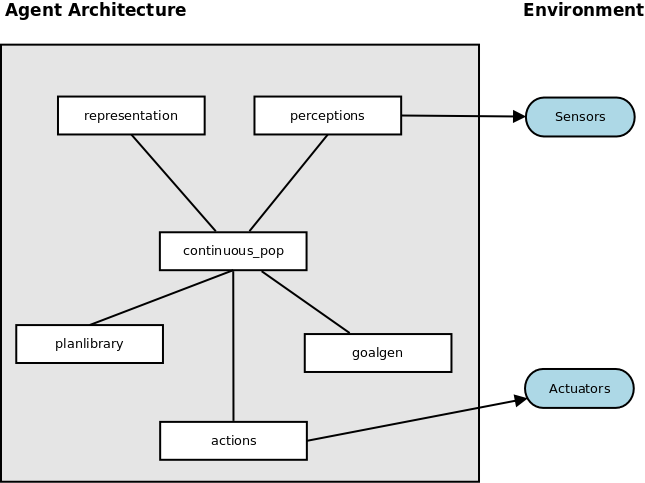
\includegraphics[width=9cm,height=8cm]{arq_modular.png}
		\caption{Arquitectura Modular del Framework de
                  Planificaci\'on Continua}
		\label{framework:modules}
	\end{figure}



	\subsection{Algoritmo de Planificaci\'on Continua}
	
	El algoritmo de planificaci\'on continua, presentado en \cite{gbraun:tesisMarioMoya}, es un
	bucle que obtiene percepciones, actualiza el estado actual 
	e intenta generar un plan.
	
	Una extensi\'on importante de la implementaci\'on es la capacidad
	de elegir un plan predefinido de una librer\'ia de planes. Por lo 
	tanto, cuando el planificador es invocado, recibe un plan inicial
	de la librer\'ia de planes. En caso que no se encuentre un plan
	acorde, se comienza con uno vac\'io.
	
	El algoritmo tiene tres estados bien definidos:
	
	\begin{itemize}
	
	\item En primer lugar, reformula las metas
	luego de procesar los deseos del agente. Entonces, se
	remueven enlaces no soportados y as\'i se evitan acciones
	con precondiciones falsas debido a cambios en los deseos
	del agente. A continuaci\'on, el algoritmo elimina acciones 
	redundantes que ya no son necesarias en el plan. Esta eliminaci\'on de 
	acciones conlleva un reemplazo de enlaces causales\footnote{Un enlace causal 
	es de la forma $A \longrightarrow^{p} B$ donde $A$ y $B$ son acciones 
	y $p$ es una proposici\'on 
	que es precondici\'on de la acci\'on $B$. La ejecuci\'on de $A$ 
	hace verdadero a $p$ para $B$ \cite{russell03:_artif_intel}.}. 
	
	\item El siguiente paso es una conducta heredada del Planificador
	de Orden Parcial (POP) \cite{gbraun:pop:1991}. Tal conducta involucra resolver 
	precondiciones abiertas. Para esto, se selecciona una precondici\'on
	e intenta resolverse agregando una nueva acci\'on o utilizando una
	ya existente.
	
	\item El \'ultimo paso del algoritmo es verificar si se ha alcanzado
	el conjunto actual de metas, es decir, no existen precondiciones
	abiertas y todos los enlaces causales van del estado \emph{Start} al
	estado \emph{Finish}\footnote{Las acciones \emph{Start} y \emph{Finish}
	pertenecen al plan inicial de la fomulaci\'on de problemas de planificaci\'on
	para el planifcador POP. Tales acciones tienen la siguiente restricci\'on de orden
	$Start \prec Finish$. \emph{Start} no tiene precondiciones y sus efectos
	son todos los literales en el estado inicial del problema. \emph{Finish}
	no tiene efectos y sus precondiciones son los literales de la
        meta del problema \cite{russell03:_artif_intel}.}.
	\end{itemize}
	

\section{Caso de estudio}
	
	Como mencionamos previamente, algunas experiencias con esta
        implementaci\'on fueron re\-a\-li\-za\-das bajo el dominio
	del F\'utbol de Robots. A continuaci\'on, se detallan las razones por las que
	este dominio fue usado para la evaluaci\'on del framework.
	
	\begin{itemize}
	
	\item Es un dominio muy desafiante y ampliamente estudiado por
	el Departamento de Teor\'ia de la Computaci\'on \cite{gbraun:cecchi09:_un_enfoq_basad_en_compet}.
	
	\item Ofrece la posibilidad de aplicar un amplio rango
	de tecnolog\'ias, como por ejemplo, video, comunicaciones y
        rob\'otica, entre otras.
	
	\item Existen en la actualidad, distintas competencias de robots
	con especificaciones y reglamentos diferentes. Entre ellas,
	podemos destacar a
	Robocup\footnote{Robocup. \url{http://www.robocup.org/}. Disponible
        en Septiembre de 2012.}, 
        FIRA\footnote{\emph{Federation of International Robot-soccer
	Association}. \url{http://www.fira.net/}. Disponible en
          Septiembre de 2012.} 
        y CAFR\footnote{Campeonato Argentino de F\'utbol de Robots.}.
	
	\item Presenta dos caracter\'isticas importantes: es un
        ambiente continuo y no determinista.
	
	\end{itemize}
	
	La utilizaci\'on de este dominio es, entonces, propicio para la
	aplicaci\'on del framework. El caso de estudio tambi\'en utiliza
	al software Rakiduam.
	
	Con el objetivo de adaptar el framework y Rakiduam, es necesario
	identificar y definir los deseos del agente, identificar acciones y metas
	y especificarlas en un lenguaje de representaci\'on de problemas de planificaci\'on.
	
	En primer lugar, y de acuerdo a la arquitectura descripta en \ref{framework:modules},
	el m\'odulo \texttt{goalgen} ge\-ne\-ra\-r\'a un conjunto nuevo de metas, consistentes
	entre s\'i, a partir de las creencias actuales del
        agente. Estas creencias incluyen las percepciones (\texttt{perceptions}) y la
	representaci\'on de acciones (\texttt{representation}). El
	m\'odulo \texttt{goalgen} tambi\'en contiene la estrategia del
	equipo y la de cada jugador seg\'un su rol. El
	m\'odulo \texttt{actions} implementa cada una de las acciones
        y las traduce a velocidades de los motores del agente mediante
        las primitivas de navegaci\'on provistas por Rakiduam.
        Por \'ultimo, el lenguaje para la representaci\'on de acciones
	y percepciones es STRIPS.
	
	Luego de esta breve descripci\'on del framework presentado por Moya,
	vamos a introducir, en la secci\'on siguiente, algunas cuestiones 
	relacionadas al rol de nuestro traductor en esta arquitectura.
	
	
\section{Integrando al Framework el Traductor PDDL desarrollado} \label{cap3:intregracion}

Como describimos en la secci\'on previa, el formalismo
que el framework usa para especificar percepciones y acciones es
STRIPS. Por otro lado, tambi\'en vimos, en el cap\'itulo \ref{pagcap2}, que
STRIPS est\'a limitado a la representaci\'on simple de acciones como una
conjunci\'on de literales. Esta \'ultima restricci\'on torna
dificultoso el modelado de acciones
complejas, por lo tanto, surje la necesidad de
tener un lenguaje de representaci\'on m\'as general, con un nivel
de abstracci\'on mayor al de STRIPS y orientado al modelado de 
dominios de aplicaci\'ones reales. Entonces, PDDL, aparece como
un potencial lenguaje de definici\'on de dominios para integrar
al framework implementado por Moya. Tambi\'en, es importante
notar que PDDL fue adoptado como un est\'andar con el 
objetivo de comparar la performance de planificadores y 
compartir diferentes problemas para un mismo dominio. De esta manera,
el framework podr\'ia ser cotejado con otras soluciones
a un mismo problema.

En base a lo expuesto, podemos definir una nueva arquitectura 
en la que integraremos nuestro traductor al Framework de
Planificaci\'on Continua. Luego, daremos un ejemplo de 
c\'omo las acciones de un agente pueden ser representadas en PDDL.

Previamente, vamos a presentar un gr\'afico que mapea el subsistema de
creencias, integrado por los m\'odulos de percepciones y 
representaci\'on, sobre el que nos proponemos trabajar.

	\begin{figure}[h!]
	\centering
		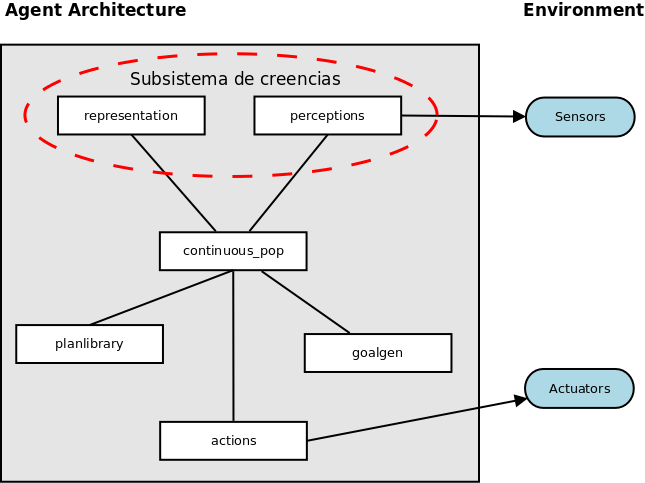
\includegraphics[width=9cm,height=8cm]{arqframework_BDI.png}
		\caption{El subsistema de creencias en la
	Arquitectura Modular del Framework.}
		\label{framework:modulesBDI}
	\end{figure}

Vemos que existen dos m\'odulos que dependen de una especificaci\'on STRIPS,
el m\'odulo \texttt{representation}, que contiene las acciones que el agente
puede ejecutar y el m\'odulo \texttt{perceptions}, que recibe percepciones
desde los sensores y las traduce a un representaci\'on STRIPS. Por lo
tanto, debido a que ambos m\'odulos constituyen el subsistema de
creencias del agente, tendremos un subsitema puramente especificado en PDDL.

En la figura \ref{framework:moduleswithPDDL}, podemos ver que 
los m\'odulos \texttt{perceptions} y \texttt{representation} 
dependen del traductor PDDL. Las percepciones
recibidas desde los sensores y la representaci\'on de las acciones del agente
son, entonces, traducidas a STRIPS. La l\'inea punteada en el gr\'afico
indica que ambos m\'odulos del subsistema de creencias dependen
de nuestro traductor.

% Ejemplo de una accion futbol en STRIPS y una en PDDL.

	\begin{figure}[h!]
	\centering
		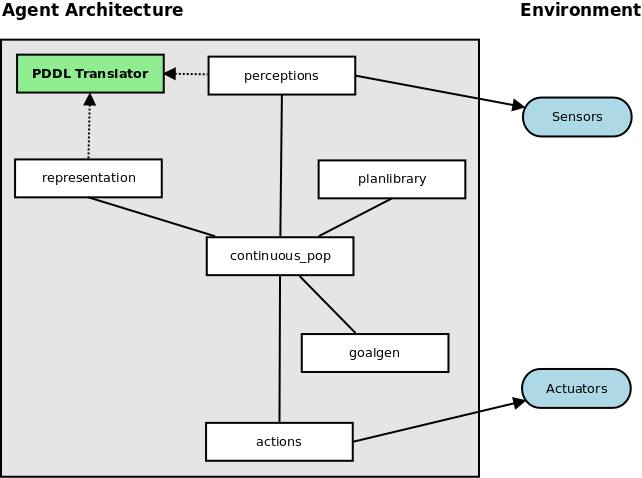
\includegraphics[width=8cm,height=7cm]{arqframework.png}
		\caption{Arquitectura del Framework y Traductor PDDL}
		\label{framework:moduleswithPDDL}
	\end{figure}


A continuaci\'on, mostramos un ejemplo de c\'omo especificamos
acciones del agente en PDDL. Primero, mostramos
la especificaci\'on de la acci\'on en STRIPS y luego,
la equivalente en PDDL. Por simplicidad, empleamos el mismo ejemplo utilizado
por Moya en \cite{gbraun:tesisMarioMoya}. 

\begin{ejemplo}%{Acciones del Agente en STRIPS}

En la acci\'on \texttt{move(Ag, Pos1, Pos2)}, el agente 
\texttt{Ag}, se desplaza de la posici\'on \texttt{pos1}
a la posici\'on \texttt{pos2}. 

 \begin{verbatim}
preconditions(move(Ag,Pos1,Pos2), [player(Ag),waiting_at(Ag,Pos1),
valid_move(Pos1,Pos2)]).
achieves(move(Ag,Pos1,Pos2),waiting_at(Ag,Pos2)).
deletes(move(Ag,Pos1,Pos2),waiting_at(Ag,Pos1)).
 \end{verbatim}
\end{ejemplo}

\begin{ejemplo}

La acci\'on equivalente en PDDL es la siguiente:

 \begin{verbatim}
(:action move
        (:parameters (?Ag ?Pos1 ?Pos2)
        (:precondition (and (player ?Ag) (waiting_at ?Ag ?Pos1)
                                         (valid_move ?Pos1 ?Pos2)))
        (:effect (and (waiting_at ?Ag ?Pos2) 
                      (not (waiting_at ?Ag ?Pos1))))
)        
 \end{verbatim}
\end{ejemplo}

El m\'odulo \texttt{perceptions} recibe el estado actual que incluye,
para el caso del F\'utbol de Robots, las coordenadas \texttt{X} e \text{Y} de los jugadores
y de la pelota. El siguiente ejemplo especifica el estado actual
usando PDDL.

\begin{ejemplo}%{Problema de f\'utbol de robots en PDDL}

Suponemos que el dominio de F\'utbol de Robots es llamado
\texttt{soccer\_domain} y los jugadores son nombrados
como \texttt{Ag} seguido de un n\'umero que lo identifica
un\'ivocamente en el problema. La meta es que el jugador
\texttt{Ag1} se desplace hacia la pelota \texttt{ball}.

 \begin{verbatim}
(define (problem soccer_problem)
(:domain soccer_domain)
(:objects Ag1 Ag2 Ag3 ball)
(:goal (carrying Ag1 ball))
(:init (at Ag1 cell1)
       (at Ag2 cell2)
       (at Ag3 cell3)
       (at ball cell4)
       (clear cell5)
       (clear cell6)
       (clear cell7))
)
 \end{verbatim}
\end{ejemplo}

Por lo tanto, proyectamos un planificador continuo cuyo lenguaje
de representaci\'on es PDDL.
\ \\

Hasta aqu\'i, hemos estudiado el lenguaje PDDL, la
implementaci\'on del Framework de Planificaci\'on Continua
desarrollado por Moya y vimos como el traductor PDDL propuesto
puede ser integrado al Framework.
En el cap\'itulo siguiente, analizaremos alternativas existentes y, a
partir del cap\'itulo \ref{pagcap6}, comenzaremos a delinear
nuestra implementaci\'on.


 %Framework

\chapter{Implementaciones Existentes} \label{pagcap4}

En el trascurso de este trabajo hemos investigado y
probado implementaciones existentes que tienen la
capacidad de interpretar PDDL como lenguaje de entrada 
y generar una especificaci\'on equivalente en un lenguaje 
destino o, simplemente, procesar sus estructuras.
Adem\'as de considerar los lenguajes fuente
y destino, al momento de abordar estas implementaciones,
tambi\'en consideramos algunas otras caracter\'isticas
importantes como lenguaje de implementaci\'on, licencias,
subconjunto de PDDL que es capaz de interpretar y
nivel de madurez de la implementaci\'on. Por \'ultimo, indicamos
las principales diferencias con nuestra propuesta.

En este cap\'itulo se detallan las implementaciones
investigadas indicando los puntos resaltados
en el parrafo anterior. En la secci\'on \ref{cap4:sec1} se describe
la alternativa planteada sobre SWI-Prolog \cite{gbraun:swiweb} y, en la secci\'on
\ref{cap4:sec2}, se estudia la gr\'amatica especificada 
en ANTLR \cite{gbraun:antlrtool}.
Por \'ultimo, en la secci\'on \ref{cap4:sec3}, se analiza una librer\'ia JAVA
adaptada para Graphplan \cite{gbraun:graphplan}.


\section{Analizador en SWI-Prolog} \label{cap4:sec1}

SWI-Prolog es una implementaci\'on del lenguaje de programaci\'on Prolog basada 
en un subconjunto de la WAM (\emph{Warren Abstract Machine}) \cite{gbraun:wam}.
Tiene un importante conjunto de caracter\'isticas entre las cuales se destacan
las librer\'ias para programaci\'on l\'ogica restringida, multi-hilos, testing unitario,
interfaces y herramientas para la Web Sem\'antica como 
RDF\footnote{\emph{Resources Description Framework}.} \cite{gbraun:w3cRDF} y 
RDFS\footnote{\emph{Resources Description Framework Schema}.} \cite{gbraun:w3cRDFS}.
SWI-Prolog est\'a bajo continuo desarrollo desde 1987 y su principal
autor es Jan Wielemaker\footnote{Jan
  Wielemaker. \url{http://staff.science.uva.nl/~wielemak/}. Disponible
en Septiembre de 2012.}.
El nombre SWI deriva del grupo \emph{Sociaal-Wetenschappelijke 
Informatica ("Social Science Informatics")} perteneciente
a la Universidad de Amsterdam.

SWI-Prolog est\'a distribuido bajo las licencias 
LGPL\footnote{\emph{Lesser GNU General Public License}.} \cite{gbraun:lgpl},
para librer\'ias del kernel y aquellas no desarrolladas
en c\'odigo Prolog y, bajo licencia GPL\footnote{\emph{GNU General Public License}.} \cite{gbraun:gpl},
para librer\'ias desarrolladas en c\'odigo Prolog.

El analizador PDDL en SWI-Prolog \cite{gbraun:prolog} fue desarrollado por
R\'obert Sas\'ak\footnote{R\'obert
  Sas\'ak. \url{http://www.sasak.sk/}. Disponible en Septiembre de 2012.} 
utilizando la libreria Prolog DCG\footnote{\emph{Definite Clause Grammar}. 
En el cap\'itulo \ref{pagcap6} introduciremos DCG.}.
La implementaci\'on est\'a incompleta ya que abarca
s\'olo un subconjunto de PDDL 3.0 y fue probada
por Sas\'ak sobre los planificadores \emph{Forward} and 
\emph{Backward Search} \cite{gbraun:Rus09}.

El analizador incluye tres m\'odulos principales. El primero, llamado \texttt{readFile.pl},
implementa un ``tokenizador''. Dicho m\'odulo toma como entrada 
un archivo de texto con la especificaci\'on PDDL y retorna un conjunto
de tokens. El m\'odulo \texttt{parseProblem.pl} recibe como entrada
la definici\'on de un problema PDDL y retorna t\'erminos Prolog.
Por \'ultimo, \texttt{parseDomain.pl}, recibe un dominio PDDL
y retorna t\'erminos Prolog equivalentes. Es importante destacar que la salida
de este analizador es una representaci\'on tipo Prolog y
no STRIPS.

A continuaci\'on, mostramos un ejemplo de una conversi\'on simple
ejecutada por el parser y luego la salida del analizador para
una instancia del  ``Mundo de Bloques''.


\begin{ejemplo}%{Parser PDDL en SWI-Prolog}

El predicado PDDL \texttt{(on ?x ?y)} es convertido
al siguiente predicado Prolog \texttt{on(?x, ?y)}.

\end{ejemplo}


\begin{ejemplo}

La salida equivalente a la definici\'on del ``Mundo de Bloques'' es la siguiente:

 \begin{verbatim}
?-parseDomain('blocks_world.pddl', O).
   O = domain(blocks,                  %name
         [strips, equality],           %requirements
         [table],                      %constants
         [on(?x, ?y),                  %predicates
	         clear(?x),
	         holding(?x),
                 ontable(?x),
	         armempty],
         [action('pickup',             %actions 
              [?x],      
              [clear(?x), armempty],
              [holding(?x)],                       
              [on(?x ?y), armempty]],
         [action('stack', 
              [?x, ?y],     
              [holding(?x), clear(?y)],
              [on(?x ?y), clear (?x), armempty],                       
              [clear(?y), holding(?x)]]
       )


?-parseProblem('problem.pddl', O).
   O = problem('blocks-4-0',            %name
              blocks,			%domain name
              [(a,b)],                  %objects
              [clear(a),                %init 
               clear(b),
               ontable(b),
               ontable(c),
               armempty, 
               on(a,c)],
              [on(a,b)],                %goal
       )
 \end{verbatim}
\end{ejemplo}

Los t\'erminos Prolog retornados por el 
analizador son predicados con una estructura general 
con un argumento por cada secci\'on PDDL en el dominio 
y problema de entrada.

Por \'ultimo, como mencionamos previamente, el analizador PDDL aqu\'i
presentado s\'olo abarca un subconjunto de la especificaci\'on
de PDDL 3.0. Los requerimientos no incluidos son:
restricciones, precondiciones negativas y disyuntivas,
acciones con restricciones de duraci\'on, predicados derivados, 
preferencias, precondiciones universales, precondiciones 
existenciales y efectos condicionales.

En base a lo expuesto, concluimos que las diferencias con nuestra
propuesta radican en el tipo de salida que presenta el traductor
implementado por Sas\'ak y en el ambiente de programaci\'on en el que
est\'a integrado. Como hemos mencionado en est\'a secci\'on, esta
implementaci\'on est\'a desarrollada un ambiente Prolog diferente
al de Ciao. Adem\'as, su lenguaje destino no es STRIPS (no distingue
entre listas de precondiciones, agregados y borrados) y no manipula 
precondiciones disyuntivas, universales ni efectos condicionales.


\section{Gram\'atica ANTLR para PDDL} \label{cap4:sec2}

%\subsection{ANTLR}

ANTLR\footnote{\emph{ANother Tool for Language Recognition}.}
es una herramienta que prove\'e un framework
para la construcci\'on de analizadores. Puede generar
analizadores l\'exicos, sint\'acticos y sem\'anticos en varios
lenguajes \emph{target}, como JAVA, C, C++ y Python, a partir
de una especificaci\'on en su propio lenguaje. B\'asicamente, el
lenguaje de ANTLR est\'a formado por una serie de reglas 
EBNF\footnote{\emph{Extended Backus Naur Form}.} \cite{gbraun:ebnf}
y un conjunto de reglas auxiliares. ANTLR toma una gr\'amatica como entrada y genera
como salida el c\'odigo generado en un lenguaje destino, como
algunos de los mencionados arriba. El lenguaje \emph{target} deseado es especificado en la 
misma gram\'atica. La herramienta est\'a disponible desde 1990, fue desarrollada 
por Terence Parr\footnote{Terence
  Parr. \url{http://www.cs.usfca.edu/~parrt/}. Disponible en
  Septiembre de 2012.} 
y es distribuida bajo licencia de software 
BSD\footnote{\emph{Berkeley Software Distribution}.} \cite{gbraun:bsd}.

ANTLR genera analizadores \emph{LL(k)} que soportan predicados sint\'acticos
y sem\'anticos permitiendo especificar muchas gram\'aticas libres y sensibles al
contexto \cite{gbraun:Chomsky1956}. Se denomina \emph{LL(k)} a la clase de
gram\'aticas para las cuales es posible construir analizadores
sint\'acticos descendentes predictivos. Estos analizadores realizan
un recorrido de izquierda a derecha, con \emph{k} s\'imbolos
de anticipaci\'on\footnote{En Ingl\'es, \emph{lookahead}.} y obtienen una
derivaci\'on a izquierda de las cadenas de entrada.

Adem\'as, ANTLR prove\'e soporte para la construcci\'on de \'arboles
gramaticales y para la recuperaci\'on y reporte de errores. 

Los tres tipos b\'asicos de herramientas procesadoras de lenguaje que 
ANTLR genera son:

\begin{enumerate}

\item {\bf Analizadores L\'exicos (\emph{lexers})}. Una analizador
l\'exico lee una cadena de caracteres, y a partir de patrones
espec\'ificos, detecta y retorna una cadena de \emph{tokens}. Tambi\'en
puede procesar espacios en blanco y comentarios, 

\item {\bf Analizadores Sint\'acticos (\emph{parsers})}. Un analizador
sint\'actico lee una cadena de tokens e identifica frases usando reglas
gramaticales. Generalmente, tambi\'en ejecuta algunas acciones sem\'anticas
para cada frase identificada, y 

\item {\bf \emph{Tree-parsers}}. Es un analizador que aplica una estructura
gramatical para guiar la traducci\'on de una entrada.
Son \'utiles durante la traducci\'on agregando atributos, 
reglas y acciones a la estructura del \'arbol. 
Estos analizadores generan como salida un Arbol
Sint\'actico Abstracto (AST)\footnote{En Ingl\'es, \emph{Abstract Syntax Tree}.}.
Un AST es una forma de c\'odigo intermedio que representa
una estructura sint\'actica y jer\'arquica del programa fuente.
 
\end{enumerate}

ANTLR permite, entonces, definir las reglas que el \emph{lexer}
debe usar para \emph{tokenizar} caracteres y las reglas
que un \emph{parser} debe usar para interpretar a los \emph{tokens}.
A continuaci\'on, explicaremos c\'omo una gram\'atica ANTLR es definida y
ejemplificaremos usando la gram\'atica ANTRL PDDL.

Los archivos ANTLR tiene una extensi\'on ``*.g''. Pueden contener
la definici\'on gramatical de uno o varios analizadores y, por cada 
analizador descripto, se generar\'a una clase en el lenguaje destino
elegido.

ANTLR PDDL fue desarrollada por Zeyn Saigol\footnote{Zeyn Saigol. 
\url{http://www.zeynsaigol.com/}. Disponible en Septiembre de 2012.} 
en el a\~{n}o 1998. La gram\'atica toma un 
subconjunto de PDDL 3.0 y genera un analizador l\'exico y un analizador
sint\'actico en c\'odigo nativo JAVA. La salida de la gram\'atica, luego
de cargarla en el entorno de desarrollo ANTLRWorks\footnote{\emph{The ANTLR GUI 
Development Environment}.} \cite{gbraun:antlrwork}, est\'a conformada por
tres archivos: un archivo de tokens, y dos ``*.java'', una
clase \emph{Lexer.java} y una clase \emph{Parser.java}.

A continuaci\'on, analizaremos la estructura de la gram\'atica
ANTLR desarrollada para el lenguaje PDDL. Empleamos algunos ejemplo extra\'idos de la definici\'on
original que puede ser encontrada en \cite{gbraun:antlrpddl}.
ANTLR PDDL tiene la siguiente estructura:

\begin{itemize}

\item {\bf Cabecera}. La cabecera, en una 
gram\'atica ANTLR, contiene c\'odigo fuente que debe ser ubicado 
previo a las clases de los analizadores en el c\'odigo generado. 
Esta secci\'on es opcional. 

El siguiente ejemplo muestra la definici\'on de una cabecera 
cuando el lenguaje \emph{target} es JAVA.

\begin{ejemplo}%{Cabecera Gramatica ANTLR}

La definici\'on de las cabeceras indican que el paquete
correspondiente debe declararse previo al resto del
c\'odigo.

 \begin{verbatim}
@parser::header {package uk.ac.bham.cs.zas.pddl.antlr;}
@lexer::header {package uk.ac.bham.cs.zas.pddl.antlr;}
 \end{verbatim}
\end{ejemplo}

\item {\bf Opciones}. Es una secci\'on
opcional, al igual que el \emph{header}, aunque es importante
en la definici\'on de un gram\'atica. Se pueden especificar
par\'ametros de ANTLR como por ejemplo, el lenguaje \emph{target}
elegido, entre otros.

\begin{ejemplo}%{Opciones Generales en ANTLR}

Las siguientes opciones son generales de la gram\'atica:

 \begin{verbatim}
options {
    output=AST;
    backtrack=true;
}
 \end{verbatim}
donde:
\begin{itemize}
\item \texttt{output=AST}: especifica
el tipo de salida del parser. Los valores v\'alidos
son \texttt{AST} y \texttt{template}. Un
\texttt{AST} es un forma de
representaci\'on intermedia que consiste de nodos
cuyas raices de los sub\'arboles son s\'olo operadores. El valor
\texttt{template} permite el uso de la librer\'ia
\texttt{StringTemplate}\footnote{La documentaci\'on oficial de esta
librer\'ia puede consultarse en
\url{http://www.antlr.org/wiki/display/ST/Introduction}. Disponible en
Septiembre de 2012.} 
para la generaci\'on de c\'odigo a partir de
determinados \emph{templates}. Esta configuraci\'on separa la
estructura de datos de c\'omo la salida es presentada. 

\item \texttt{backtrack=true}: activa
la recuperaci\'on de errores reglas no son
exitosas. En este caso, ning\'un error es reportado durante
el an\'alisis.
\end{itemize}

Ning\'un lenguaje \emph{target} es especificado en esta
secci\'on pero, por defecto, ANTLR asume que el c\'odigo destino
es JAVA.
\end{ejemplo}

\item \texttt{tokens}: En esta secci\'on pueden definirse dos tipos de \emph{tokens}. 
Los primeros, llamados ``i\-ma\-gi\-na\-rios'', no se corresponden con un s\'imbolo de 
entrada real y pueden ser usados como \emph{labels} para agrupar \emph{tokens} 
de la entrada real. Estos \emph{tokens} puede ser referenciados desde
las reglas gramaticales. Adem\'as, tambi\'en pueden especificarse
\emph{tokens} llamados ``literales'' que suelen
usarse para asignar alg\'un \emph{label} a \emph{tokens} de la entraba.

\begin{ejemplo}%{Tokens ANTLR PDDL}

El siguiente es un subconjunto de \emph{tokens} definidos
en la gram\'atica ANTLR.

 \begin{verbatim}
tokens {
    DOMAIN;
    DOMAIN_NAME;
    REQUIREMENTS;
    TYPES;
    CONSTANTS;
    PREDICATES;
    ACTION;
    PROBLEM;
    PROBLEM_NAME;
    PROBLEM_DOMAIN;
    OBJECTS;
    INIT;
    PRECONDITION;
    EFFECT;
    AND_GD;
    OR_GD;
    NOT_GD;
    FORALL_GD;
    AND_EFFECT;
    FORALL_EFFECT;
    WHEN_EFFECT;
    GOAL;
}
 \end{verbatim}
\end{ejemplo}

\item \texttt{members}: en esta secci\'on se definen m\'etodos 
y variables que luego formar\'an parte de la clase del analizador.

\begin{ejemplo}%{Codigo Nativo en ANTLR PDDL}

La gram\'atica define los siguientes m\'etodos para la clase
\emph{parser}:

 \begin{verbatim}
@parser::members {
    private boolean wasError = false;
    public void reportError(RecognitionException e) {
	            wasError = true;
	            super.reportError(e);
    }
    public boolean invalidGrammar() {
	            return wasError;
    }
}
 \end{verbatim}
\end{ejemplo}

\item {\bf Reglas}: la \'ultima secci\'on de la gram\'atica
es la definici\'on de reglas gramaticales. ANTLR PDDL
incluye reglas para el \emph{lexer}, que se utilizar\'an
para la identificaci\'on de tokens y reglas para
el \emph{parser}, que son patrones con el objetivo de
identificar frases del lenguaje usando los tokens
generados por el \emph{lexer}. Las reglas est\'an en
notacion EBNF.

\begin{ejemplo}%{Reglas L\'exicas en ANTLR PDDL}

Las siguientes son algunas de las reglas definidas 
para el an\'alisis l\'exico. Las reglas est\'an acotadas
al subconjunto de PDDL definido para el presente trabajo.

 \begin{verbatim}

REQUIRE_KEY
    : ':strips'
    | ':disjunctive-preconditions'
    | ':equality'
    | ':universal-preconditions'
    | ':quantified-preconditions'
    | ':conditional-effects'
    ;

NAME:    LETTER ANY_CHAR* ;

fragment LETTER:	'a'..'z' | 'A'..'Z';
fragment ANY_CHAR: LETTER | '0'..'9' | '-' | '_';

VARIABLE : '?' LETTER ANY_CHAR* ;

NUMBER : DIGIT+ ('.' DIGIT+)? ;

fragment DIGIT: '0'..'9';

LINE_COMMENT
    : ';' ~('\n'|'\r')* '\r'? '\n' { $channel = HIDDEN; }
    ;

WHITESPACE
    :   (   ' '
        |   '\t'
        |   '\r'
        |   '\n'
        )+
        { $channel = HIDDEN; }
    ;
 \end{verbatim}
\end{ejemplo}

\begin{ejemplo}%{Reglas Sint\'acticas en ANTLR PDDL}

Las siguientes son algunas de las reglas definidas
para el an\'alisis sint\'actico. Las primeras, corresponden
a dominios PDDL (\texttt{domain} y \texttt{actionDef}) 
y las \'ultimas, a problemas PDDL (\texttt{problem}). 

 \begin{verbatim}
pddlDoc : domain | problem;}

domain
    : '(' 'define' domainName
      requireDef?
      typesDef?
      constantsDef?
      predicatesDef?
      functionsDef?
      constraints?
      structureDef*
      ')'
      -> ^(DOMAIN domainName requireDef? typesDef?
                constantsDef? predicatesDef? functionsDef?
                constraints? structureDef*)
    ;
    
actionDef
	: '(' ':action' actionSymbol
	      ':parameters' '(' typedVariableList ')'
           actionDefBody ')'
       -> ^(ACTION actionSymbol typedVariableList actionDefBody)
    ;
    
problem
	: '(' 'define' problemDecl
	  problemDomain
      requireDef?
      objectDecl?
      init
      goal
      probConstraints?
      metricSpec?
      ')'
      -> ^(PROBLEM problemDecl problemDomain requireDef? objectDecl?
      		init goal probConstraints? metricSpec?)
    ;

 \end{verbatim}
\end{ejemplo}

\end{itemize}	


De manera similar a la secci\'on anterior, las diferencias con
nuestra propuesta radican en el tipo de soluci\'on que ofrece la
gram\'atica ANTLR y el lenguaje en el que est\'a implementada. 
Si bien, es una alternativa flexible a
los cambios en la gram\'atica PDDL de entrada, los analizadores,
generados a partir de la gram\'atica ANTLR PPDL, no
realizan ninguna traducci\'on de PDDL a STRIPS.

%A continuaci\'on, vamos a introducir la \'ultima implementaci\'on
%investigada, la libreria \emph{PDDL4J} desarrollada en JAVA.


\section{Librer\'ia PDDL4J} \label{cap4:sec3}

PDDL4J es una librer\'ia de c\'odigo abierto 
distribuida bajo licencia CECILL \cite{gbraun:cecill} y fue de\-sa\-rro\-lla\-da por 
Damien Pellier\footnote{Damien Pellier. \url{http://www.math-info.univ-paris5.fr/~pellier/home}. Disponible
en Septiembre de 2012.}. 

El prop\'osito de PDDL4J es facilitar la implementaci\'on JAVA
de planificadores basados en PDDL. La librer\'ia contiene un
analizador de la especificaci\'on PDDL 3.0 con todas las clases
necesarias para la manipulaci\'on de sus prinicipales caracter\'isticas. Acepta un
importante conjunto de requerimientos PDDL entre los que se
encuentran los requerimientos presentados para nuestro trabajo
y se agregan tipos, precondiciones negativas y existenciales,
fluents, predicados derivados, acciones con tiempo,
preferencias y restricciones.

La propuesta de Pellier incluye una implementaci\'on
del planificador Graphplan usando PDDL4J. Lo novedoso de esta implementaci\'on
es que retorna, junto con el plan final, algunas estad\'isticas 
sobre la ejecuci\'on del algoritmo con el objetivo de comparar esta soluci\'on con
otras implementaciones. 

Graphplan es una planificador de prop\'osito general para dominios
especificados en STRIPS. Dado un problema, Graphplan
construye, expl\'icitamente, una estructura llamada
\emph{Grafo de Pla\-ni\-fi\-ca\-ci\'on} que es explorado para obtener un plan
que resuelva un problema, si es que \'este existe. Graphplan
fue creado por Avrim Blum\footnote{Avrim
  Blum. \url{http://www.cs.cmu.edu/~avrim/home.html}. Disponible en
  Septiembre de 2012.}, 
Merrick Furst\footnote{Merrick
  Furst. \url{http://www.scs.gatech.edu/people/merrick-furst}. Disponible
en Septiembre de 2012.} 
y John Langford\footnote{John 
Langford. \url{http://hunch.net/~jl/}. Disponible en Septiembre de 2012.}.

A continuaci\'on, mostramos la salida de Graphplan
luego de ejecutarlo sobre el dominio y problema
PDDL de una instancia del ``Mundo de Bloques''.

\begin{ejemplo}%{Graphplan usando PDDL4J}

Dada la meta \texttt{on(a b)} y las acciones
\texttt{stack} y \texttt{pickup},
ejecutamos Graphplan pasando, como argumentos
del planificador, los archivos ``*.pddl'' correspondientes.

 \begin{verbatim}
java -server -jar graphplan.jar domain.pddl problem.pddl
 \end{verbatim}

Luego, el resultado de la planificaci\'on es el siguiente:

 \begin{verbatim}
Parsing domain "bkw" done successfully ...
Parsing problem "pb1" done successfully ...

Preprocessing ...

time:    0,        5 facts,          0 and exlusive pairs (0,0003s)
                   7 ops,            7 exlusive pairs
time:    1,        7 facts,          7 and exlusive pairs (0,0006s)
                  11 ops,           35 exlusive pairs

goals first reachable in 2 times steps


found plan as follows:

time step    0: PICKUP a
time step    1: STACK a b

number of actions tried :            2 
number of noops tried   :            1 

Time spent :     0,01 seconds preprocessing 
                 0,00 seconds build graph 
                 0,00 seconds calculating exclusions 
                 0,00 seconds searching graph 
                 0,01 seconds total time 

 \end{verbatim}

La salida retorna el plan resultante para alcanzar
la meta e informaci\'on relacionada al tiempo de ejecuci\'on
del algoritmo. Entre la informaci\'on mostrada, podemos destacar
que el problema y el dominio en PDDL fue analizado exitosamente, 
la meta fue alcanzada con s\'olo dos acciones \texttt{pickup a} y
\texttt{stack a b}, y el tiempo
total para alcanzar la soluci\'on fue de 0.01 segundos.
\end{ejemplo}

Teniendo en cuenta lo analizado en esta secci\'on, concluimos que la
diferencia con nuestra propuesta radica en que la soluci\'on,
desarrollada por Pellier, es una librer\'ia JAVA y
su prop\'osito es facilitar la implementaci\'on de planificadores
en el mismo lenguaje. Este no es el caso del Pla\-ni\-fi\-ca\-dor Continuo
ya que est\'a desarrollado, \'integramente, en Ciao Prolog. Es esperable
una mejor integraci\'on si el traductor, propuesto en este
trabajo, es implementado en el mismo ambiente del Planificador Continuo. 
\ \\

En resumen, en este cap\'itulo hemos presentado y analizado tres 
implementaciones existentes que fueron
estudiadas en el trascurso de este trabajo. 
A partir del pr\'oximo cap\'itulo, vamos a iniciar el an\'alisis de nuestro traductor
PDDL y, para esto, comenzaremos definiendo el marco te\'orico subyacente.




 %Implementaciones Existentes

\chapter{Traducci\'on de requerimientos PDDL} \label{pagcap5}
	
	En el cap\'itulo \ref{pagcap2} analizamos el lenguaje STRIPS. 
        Este formalismo describe acciones en
        t\'erminos de precondiciones y efectos. Las precondiciones 
        de las acciones son conjunciones de literales positivos, al igual que los
        estados inicial y final. Los efectos de las acciones son
        expresados como una conjunci\'on de literales. Esta
        definici\'on de STRIPS,
        m\'as el predicado de igualdad y su negaci\'on, conforman el
        lenguaje de representaci\'on soportado por el Planificador
        Continuo presentado en el cap\'itulo \ref{pagcap3}. Luego, 
        estudiamos el lenguaje PDDL e identificamos los
        siguientes requerimientos que est\'an siendo considerados para el
        desarrollo del presente trabajo: igualdad, efectos
        condicionales, precondiciones disyuntivas y precondiciones universales.

        En este cap\'itulo vamos a identificar y definir variantes
        para STRIPS. Tales variantes surjen adicionando los
        requerimientos anteriores a la especificaci\'on de dicho lenguaje. 
        Adem\'as, estableceremos una notaci\'on
        equivalente en PDDL para estas variantes y analizaremos la
        teor\'ia subyacente. Por \'ultimo, propondremos formas de
        procesar cada variante para una posterior implementaci\'on en
        el traductor propuesto.
	
	La organizaci\'on del presente cap\'itulo es la siguiente. 
        En la secci\'on \ref{cap5:inicial} se define un marco
        te\'orico incluyendo resultados preliminares, las nociones
	de {\bf esquemas de compilaci\'on} y {\bf compilabilidad} y 
        algunos supuestos de simplificaci\'on. En las secciones subsiguientes 
        se discute, de manera te\'orica, la traducci\'on de cada una
	de las variantes STRIPS identificadas. 
        En la secci\'on \ref{cap5:strips} se muestra la traducci\'on \emph{trivial} para
	STRIPS est\'andar. Posteriormente, en la
        secci\'on \ref{cap5:pddll}, se analiza STRIPS con literales
        negativos y el predicado de igualdad. A este formalismo lo
        denotaremos PDDL$_{L}$. En la secci\'on \ref{cap5:efectoscond}
	se analiza STRIPS con efectos condicionales, 
        STRIPS$_{\emph{C}}$ y su equivalente PDDL$_{\emph{C}}$. La
        secci\'on \ref{cap5:preconddisy} presenta STRIPS con precondiciones disjuntivas, 
	STRIPS$_{D}$ y PDDL$_{D}$. 
        En la secci\'on \ref{cap5:precondUniv} se introduce
	uno de los resultados m\'as importantes de nuestra
	investigaci\'on. Este resultado formaliza y demuestra una nueva variante
	de STRIPS que incluye precondiciones cuantificadas
	universalmente. Tal variante es llamada
        STRIPS$_{\emph{u}}$ con su equivalente PDDL$_{\emph{u}}$.
        Por \'ultimo, todos los ejemplos en este cap\'itulo concluyen con la representaci\'on
        STRIPS para cada dominio traducido. Tal representaci\'on
        es similar a la definida para el Planificador Continuo.
	
	
\section{Marco Te\'orico} \label{cap5:inicial}

	
	Existe un \emph{trade-off}\footnote{Un balance aceptable entre 
	dos cosas opuestas con el fin de lograr un objetivo.} entre la 
	expresividad y la ``gesti\'on''\footnote{En Ingl\'es, \emph{manageability}.} 
	de un lenguaje formal de definici\'on de dominios de planificaci\'on.
	Un lenguaje pr\'actico deber\'ia tener un nivel lo m\'as alto posible 
	para poder representar problemas de una manera natural, exacta y simple. 
	Sin embargo, mientras m\'as se incrementa la complejidad de lenguaje en cuesti\'on, 
	m\'as se incrementa la dificultad para resolver el problema
	por parte de los planificadores. 
        En \cite{gbraun:Gazen97combiningthe}, Gazen y Knoblock, definen dos enfoques posibles 
	que permiten considerar un lenguaje m\'as expresivo de representaci\'on de dominios. 
	El primero, enuncia que para soportar un lenguaje m\'as
	expresivo se debe extender el algoritmo de planificaci\'on. 
	Mientras que el segundo enfoque, implica desarrollar un
	preprocesador que traduzca un dominio representado en un
	lenguaje m\'as expresivo a uno m\'as simple. 
	Si bien, esta \'ultima propuesta no podr\'ia manejar 
        constructores m\'as expresivos de manera tan eficiente, 
        es m\'as simple desde el punto de vista conceptual. 
	Consideramos esta segunda propuesta para desarrollar el
	presente trabajo.

        Esta secci\'on presenta resultados y definiciones,
        introducidas por Nebel en \cite{gbraun:Nebel2000onthe} y \cite{gbraun:Nebel:2001:EPP}, 
        y adaptadas a las necesidades de nuestra
        implementaci\'on.
	

        \subsection{Esquemas de Compilaci\'on}
	
	En primer lugar, introducimos la
        definici\'on de instancia de planificaci\'on para luego continuar el estudio
        sobre los esquemas de compilaci\'on.

	%%%%%% Instancia de planificacion

        \begin{definition}

        Sea $\Sigma$ un conjunto finito de \texttt{\'atomos
        proposicionales}, $O$ un conjunto finito de operadores y
        $\hat{\Sigma} = \top \cup \bot \cup literales(\Sigma)$ donde,
        $\top$ denota \texttt{verdadero}, $\bot$ denota
        \texttt{falso} y $literales(\Sigma)$ es el conjunto de
        literales definidos sobre $\Sigma$.

	Una {\bf instancia de planificaci\'on} es una 
	tupla $\Pi = \left\langle \Xi,I,G \right\rangle$ donde:
	
	\begin{itemize}
	
	\item $\Xi = \left\langle \Sigma,O \right\rangle $ es una estructura 
	de dominio que consiste de un conjunto finito de \'atomos proposicionales 
	y un conjunto finito de operadores,
	
	\item $I \subseteq \Sigma $ es el estado inicial, y
	
	\item $G \subseteq \hat{\Sigma} $ es la especificaci\'on de la meta.
	
	\end{itemize}
	
	\end{definition}

        La estructura $\Xi$ es el dominio de planificaci\'on compuesto
        por acciones (tambi\'en llamadas operadores en la
        bibliograf\'ia) mientras que los conjuntos $I$ y $G$ 
        conforman la especificaci\'on del problema de planificaci\'on.
        
        A continuaci\'on, damos una noci\'on intuitiva del
        concepto de esquemas de compilaci\'on y, posteriormente,
        presentamos este concepto de manera formal, adaptando la
        definici\'on propuesta por Nebel.

        Un formalismo de planificaci\'on $X$ es tan expresivo como otro 
	formalismo $Y$ si, los dominios de planificaci\'on y los planes formulados 
	en $Y$, son expresables en $X$ de manera
	concisa. B\'asicamente, un esquema de compilaci\'on es 
	una soluci\'on que preserva el mapeo entre las estructuras de
	dominio en el formalismo $X$ y en el formalismo $Y$. La
        siguiente definici\'on expresa este concepto.
	
	\begin{definition}
	
	Un {\bf esquema de compilaci\'on\footnote{En Ingl\'es, \emph{compilation
	scheme}.}} de $X$ a $Y$ es una tupla de funciones 
	$f = \left\langle f_{\xi},f_{i},f_{g} \right\rangle $ que inducen una funci\'on $F$
	de instancias de $X$, $\Pi = \left\langle \Xi,I,G \right\rangle $, a instancias de $Y$,
	$F(\Pi)$, como sigue:
	
	\begin{center}
		
	$F(\Pi) = \left\langle f_{\xi}(\Xi),I \cup f_{i}(\Xi),G \cup f_{g}(\Xi) \right\rangle $
	
	\end{center}
		
	y satisfacen las siguientes condiciones:
		
	\begin{itemize}
		
	\item existe un plan para $\Pi$, si y s\'olo si, existe un plan
          para $F(\Pi)$, y
		
	\item el tama\~{n}o de los resultados de $f_{\xi},f_{i}$ y $f_{g}$ es 
	polinomial en el tama\~{n}o de los argumentos.
		
	\end{itemize}
	
	\end{definition}

        Si bien, esta definici\'on establece condiciones referidas a la complejidad
        computacional de las funciones $f_{\xi},f_{i}$ y $f_{g}$, esto no
        es un factor limitante en nuestra investigaci\'on. Sin embargo,
        en el caso general, procuramos definir esquemas de compilaci\'on
        eficientes en t\'erminos de complejidad computacional. 

        En este sentido, establecemos los siguientes supuestos relacionados
        a este tipo de mapeos:

        \begin{enumerate}

        \item No haremos ninguna restricci\'on sobre los recursos
        computacionales, por lo tanto, un
	an\'alisis exhaustivo de la complejidad computacional queda
	fuera del alcance del presente trabajo.

        \item Las estructuras de dominio son traducidas de manera
        independiente respecto de la descripci\'on del estado
        inicial y la meta del problema de planificaci\'on.

        \item No existe ninguna restricci\'on sobre el tama\~{n}o
        de los dominios involucrados en el mapeo.

        \item La longitud del plan resultante es preservada en
        \emph{cierto grado}. Este supuesto ser\'a retomado m\'as adelante
        cuando expliquemos compilabilidad.
        
        \end{enumerate}


        En la siguiente secci\'on analizaremos y definiremos
        formalmente la noci\'on de compilabilidad.


        \subsection{Compilabilidad}

        A partir de los conceptos que aparecen en \cite{gbraun:Nebel:2001:EPP}, vamos a
        enunciar una definici\'on relacionada al tama\~{n}o de los planes.
	
	\begin{definition}
	
	Sea \texttt{f} un esquema de compilaci\'on, $\Delta$ un
	plan que resuelve la instancia de planificaci\'on $\Pi$ y $\Delta^{'}$ un plan que
	resuelve la instancia de planificaci\'on $F(\Pi)$. Mediante 
	$||\Delta||$ denotamos el tama\~{n}o de un plan para el
	formalismo fuente y mediante $||\Delta^{'}||$ denotamos el tama\~{n}o de
	un plan para el formalismo destino.
	Asimismo, mediante $||\Pi||$ se denota el tama\~{n}o de la instancia.
	
        Entonces:
	
	\begin{itemize}
	
	\item \texttt{f} es un {\bf esquema de compilaci\'on que preserva exactamente el tama\~{n}o del plan}
	si $||\Delta^{'}|| \leq ||\Delta|| + k $, para alguna
	constante entera positiva $k$. 
	
	\item \texttt{f} es un {\bf esquema de compilaci\'on que preserva linealmente el tama\~{n}o del plan}
	si $||\Delta^{'}|| \leq c x ||\Delta|| + k $, para las
	constantes positivas $c$ y $k$.
	
	\item \texttt{f} es un {\bf esquema de compilaci\'on que preserva polinomialmente el tama\~{n}o del plan}
	si $||\Delta^{'}|| \leq p(||\Delta||, ||\Pi||) $, para alg\'un
	polinomio $p$.
	
	\end{itemize}
	\end{definition}
	
        A continuaci\'on, formalizamos la relaci\'on de
        compilabilidad\footnote{En Ingl\'es, \emph{compilability}.}.
	
	\begin{definition}
	
	Un formalismo de planificaci\'on $X$ es {\bf compilable} al formalismo 
	$Y$, expresado como $X \preccurlyeq^{x} Y$, si y s\'olo si,
	existe un esquema de compilaci\'on de $X$ a $Y$.
	
	Entonces:
	
	\begin{itemize}
	
	\item Si $X \preccurlyeq^{1} Y$, entonces el tama\~{n}o del plan es preservado exactamente.
	
	\item Si $X \preccurlyeq^{c} Y$, entonces el tama\~{n}o del plan es preservado 
	linealmente (en $||\Delta||$).
	
	\item Si $X \preccurlyeq^{p} Y$, entonces el tama\~{n}o del plan es preservado 
	polinomialmente (en $||\Delta||$ y $||\Pi||$).
	
	\item Si $X \preccurlyeq^{x}_{p} Y$, entonces la compilaci\'on
        es en tiempo polinomial y el tama\~{n}o del plan es preservado 
	polinomialmente (en $||\Delta||$ y $||\Pi||$).
	
	\end{itemize}
	
	\end{definition}
	
	Los casos en los que la compilaci\'on de formalismos 
	preserva el tama\~{n}o de un plan, ya sea exacta o linealmente,
	indican que el formalismo destino que estamos considerando 
	es, al menos, tan expresivo como el formalismo fuente.
	Sin embargo, si un esquema de compilaci\'on requiere 
	de un crecimiento polinomial respecto al tama\~{n}o de los planes,
	entonces el formalismo fuente es m\'as expresivo que 
	el formalismo destino.
	
	Por \'ultimo, en \cite{gbraun:Nebel:2001:EPP}, se enuncian dos propiedades importantes
	para la relaci\'on de com\-pi\-la\-bi\-li\-dad:
	

	\begin{proposition} \label{cap5:reflex} 
	
	Las relaciones $\preccurlyeq^{x}$ y $\preccurlyeq^{x}_{p}$ 
	son reflexivas y transitivas.
	
	\end{proposition}
	
	\begin{proposition}  
	
	Si $X \sqsubseteq Y$, entonces $X \preccurlyeq^{1}_{p} Y$.
	
	\end{proposition}
	

	
	
	%%%%%%%%%%%%%%%%%%%%%%%%%%%%%%%%%%%%%%%%%%%%%%%%%
	

	
        En las siguientes secciones clasificaremos y ejemplificaremos 
        las variantes STRIPS con\-si\-de\-ra\-das y propondremos una
        notaci\'on equivalente para PDDL. Adem\'as, usando la
        relaci\'on de compilabilidad, definiremos esquemas de
        compilaci\'on que luego ser\'an implementados en nuestro
        traductor. Para esto, proponemos las capas de
        traducci\'on que se indican en la figura \ref{gbraun:layers}.


        \begin{figure}[h!]
	\centering
		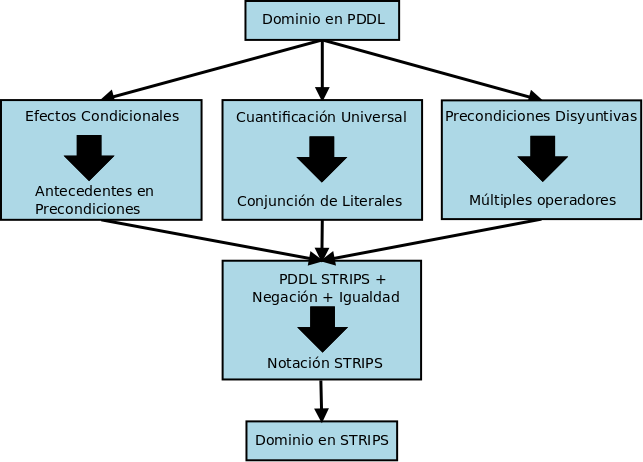
\includegraphics[width=10cm,height=9cm]{capastrad.png}
		\caption{Capas de Traducci\'on}
		\label{gbraun:layers}
	\end{figure}


%	\section{STRIPS y STRIPS$_{L}$} \label{cap5:stripsigualdad}

        \section{PDDL$_{STRIPS}$} \label{cap5:strips}


        El STRIPS est\'andar, estudiado en el cap\'itulo \ref{pagcap2} y
        definido por Russell y Norving en \cite{gbraun:Rus09},
        es el formalismo m\'as b\'asico de esta
        clasificaci\'on en t\'erminos de expresividad. B\'asicamente,
        describe acciones mediante precondiciones y efectos.
        Las precondiciones son conjunciones de literales positivos al
        igual que los estados inicial y final. Los efectos son
        expresados como una conjunci\'on de literales. Los literales positivos
        son inclu\'idos en la lista de agregados y los negativos en la
        lista de borrados de la acci\'on. STRIPS est\'andar no permite
        efectos condicionales, disyunci\'on ni cuantificaci\'on
        universal en precondiciones.

        A continuaci\'on, estudiaremos la traducci\'on de STRIPS
        expresado en PDDL.
	

        \begin{proposition} \label{cap5:trivial}
	$STRIPS \preccurlyeq^{1} STRIPS$.
        \end{proposition}

        \begin{proof}
        Por propiedad reflexiva de la relaci\'on de compilabilidad,
        proposici\'on \ref{cap5:reflex}, concluimos que STRIPS
        es \emph{compilable} a STRIPS preservando exactamente el
        tama\~{n}o de los planes. 
        \end{proof}

        Luego, si denotamos como PDDL$_{STRIPS}$ al formalismo PDDL
        acotado a la expresividad de STRIPS y lo reemplazamos 
        en la proposici\'on anterior, podemos concluir que:

        \begin{corolario} \label{cap5:trivial}
	$PDDL_{STRIPS} \preccurlyeq^{1} STRIPS$
        \end{corolario}
        
        Por lo tanto, PDDL$_{STRIPS}$ es \emph{compilable} a
        STRIPS est\'andar preservando exactamente el tama\~{n}o de
        los planes. Este lenguaje es el m\'as b\'asico en t\'erminos de
        expresividad.

        Veamos, mediante un ejemplo, c\'omo
        PDDL$_{STRIPS}$ es traducido a STRIPS. 

        \begin{ejemplo}

        Dada una instancia del problema del ``Mundo de Bloques'' en
        PDDL$_{STRIPS}$, la traducci\'on procede adicionando efectos
        negados a la lista de borrados y efectos positivos a la lista
        de agregados de la especificaci\'on STRIPS.

        \begin{verbatim}
% Dominio PDDL
(define (domain bkw)
(:requirements :strips)
(:predicates (clear ?x)
             (ontable ?x)
             (armempty)
             (holding ?x)
             (on ?x ?y))

(:action pickup
  :parameters (?ob)
  :precondition (and (clear ?ob) (armempty))
  :effect (and (holding ?ob) (not (clear ?ob)) (not (armempty))))

(:action stack
  :parameters  (?ob ?underob)
  :precondition (and  (clear ?underob) (holding ?ob))
  :effect (and (clear ?ob) (on ?ob ?underob) (armempty)
               (not (clear ?underob)) (not (holding ?ob))))
)

% Problema PDDL
(define (problem pb1)
   (:domain bkw)
   (:objects a b c)
   (:goal (on a b))
   (:init (ontable c) (ontable b) 
          (on a c) (clear a) (clear b) (armempty))
)
        \end{verbatim}
        La representaci\'on en STRIPS del problema anterior es la
        siguiente:
        \begin{verbatim}

% pickup(X,Y)
Precondiciones: clear(X), armempty
Borrados: clear(X), armempty
Agregados: holding(X)

% stack(X,Y)
Precondiciones: clear(Y), holding(X)
Borrados: clear(Y), holding(X)
Agregados: armempty, clear(X), on(X,Y)


% Problema STRIPS
holds(ontable(c),init)
holds(ontable(b),init)
holds(on(a,c),init)
holds(clear(a),init)
holds(clear(b),init)
holds(armempty,init)
        \end{verbatim}
        \end{ejemplo} 

        En base a lo expuesto, podemos concluir que PDDL$_{STRIPS}$ es soportado por el
        Planificador Continuo.



%	\subsection{STRIPS$_{L}$}

        \section{PDDL$_{L}$} \label{cap5:pddll}

        En el caso del predicado de igualdad, el escenario que se presenta es
        diferente. STRIPS est\'andar no soporta el uso de este
        predicado en las precondiciones, no obstante, es aceptado
        en algunas variantes STRIPS. 
        Ocurre algo similar para el caso de la negaci\'on ya que no est\'a incluida en
        la definici\'on de STRIPS. Algunos planificadores aceptan
        negaci\'on pero, \'unicamente, del predicado igualdad. Este es el caso del lenguaje de 
        representaci\'on del Planificador Continuo.          

        Por su parte, PDDL si permite incluir negaci\'on en las precondiciones
        y en las metas de los
        problemas de planificaci\'on posibilitando la definici\'on de
        acciones como indicamos a continuaci\'on:

        \begin{ejemplo}%{Negaci\'on de literales en precondiciones}
        
        Podemos modelar en PDDL la acci\'on \textt{stack} del 
        ``Mundo de Bloques'' permitiendo que un bloque, \textt{?X}, sea apilado 
        sobre otro, \textt{?Z}, si \textt{?Z} no es un bloque.

        \begin{verbatim}
(:action stack
   :parameters (?X ?Y ?Z)
   :precondition (and (clear ?X) (clear ?Z) (on ?X ?Y) (not (block ?Z)))
   :effects (and (on ?X ?Z) (clear ?Y) (not (on ?X ?Y))) 
)
        \end{verbatim}
        \end{ejemplo}

        Sin embargo, como mencionamos al
        inicio de esta secci\'on, esta caracter\'istica no es
        soportada directamente por STRIPS est\'andar, por lo tanto, es
        necesaria una traducci\'on. 

        La adici\'on de la negaci\'on a STRIPS da lugar a otra variante
        del formalismo llamada STRIPS$_{L}$. Esta variante tiene la
        particularidad, a diferencia de STRIPS
        est\'andar, de permitir negaci\'on de literales en las
        precondiciones. 

        A continuaci\'on, enunciamos, sin
        demostrar, el siguiente resultado postulado por Nebel 
        en \cite{gbraun:Nebel2000onthe}:


        \begin{proposition} \label{cap5:stripsLtostrips}
        $STRIPS_{L} \preccurlyeq^{1}_{p} STRIPS$
        \end{proposition}

        A partir de este resultado, concluimos que STRIPS$_{L}$ es
        \emph{compilable} a STRIPS, en tiempo
        polinomial y el tama\~{n}o de los planes es
        preservado exactamente. 
        
        En este sentido, tambi\'en definimos a PDDL$_{L}$ como el formalismo obtenido de restringir
        PDDL al requerimiento de negaci\'on (STRIPS
        est\'a impl\'icito por ser el requerimiento por defecto de
        PDDL). Dado que PDDL$_{L}$ es lo mismo que
        STRIPS$_{L}$ en t\'erminos de nivel expresivo y, por  
        la proposici\'on \ref{cap5:stripsLtostrips}, podemos concluir que:

        \begin{corolario} 
        $PDDL_{L} \preccurlyeq^{1}_{p} STRIPS$
        \end{corolario}

        Es decir, PDDL$_{L}$ es \emph{compilable} a STRIPS en tiempo
        polinomial y el tama\~{n}o de los planes es
        preservado exactamente. 

        La definici\'on original de STRIPS$_{L}$ enunciada por Nebel
        s\'olo establece el uso de
        literales negativos en precondiciones, pero nada concluye
        sobre la aceptaci\'on, o no, del predicado de igualdad. Adem\'as, la
        igualdad no es soportada por STRIPS est\'andar, aunque s\'i es
        soportada por el lenguaje de representaci\'on del
        Planificador Continuo.

        Entonces, con el objetivo de incluir el predicado en el contexto de un
        subconjunto acotado de PDDL, en este trabajo de tesis, vamos a considerar
        el predicado de igualdad como parte de STRIPS$_{L}$ y, en
        consecuencia, de PDDL$_{L}$

        El pr\'oximo ejemplo muestra c\'omo modelar acciones
        en PDDL$_{L}$ usando el predicado de igualdad:

        \begin{ejemplo}%{Igualdad en PDDL}

        La acci\'on \texttt{stack}
        permite apilar un bloque s\'olo si el destino es 
        la mesa. \texttt{table} es una constante.

	\begin{verbatim}
(:action stack
   :parameters (?X ?Y)
   :precondition (and (clear table) (= ?Y table)) 
   :effect (and (on ?X table) (not (clear table)))
)                
	\end{verbatim}
	\end{ejemplo}
  
        Por \'ultimo, es necesario definir una restricci\'on
        importante sobre PDDL$_{L}$ para que pueda ser \'integramente
        soportado por el Planificador Continuo. 
        Dicha restricci\'on es impuesta sobre el requerimiento
        de negaci\'on:

        \begin{itemize}

        \item Permitiremos el uso del \texttt{not}, en precondiciones, s\'olo cuando
        es aplicado junto con el pre\-di\-ca\-do de igualdad, tal es el caso
        del t\'ermino \texttt{(not (= ?Y ?Z))}\footnote{Existen otras
        alternativas para tratar con la negaci\'on en precondiciones
        como la presentada por Gazen y
        Knoblock \cite{gbraun:Gazen97combiningthe} para el
        planificador Graphplan. Sin embargo, un an\'alisis exhaustivo
        de estas alternativas est\'a fuera del alcance de esta investigaci\'on.}.

        \end{itemize}

        Veamos, mediante un ejemplo, c\'omo traducir PDDL$_{L}$ a la
        representaci\'on STRIPS del Pla\-ni\-fi\-ca\-dor Continuo.

        \begin{ejemplo}
        
        Traducimos la siguiente acci\'on con el predicado de igualdad
	a notaci\'on STRIPS:

	\begin{verbatim}
(:action stack
   :parameters (?X ?Y)
   :precondition (and (clear table) (= ?Y table)) 
   :effect (and (on ?X table) (not (clear table)))
)                
	\end{verbatim}

        \begin{verbatim}
% stack(X,Y)
Precondiciones: clear(table), Y == table
Borrados: clear(table)
Agregados: on(X,table)             
	\end{verbatim}

        Y la negaci\'on del predicado de igualdad en precondiciones:

	\begin{verbatim}
(:action stack
   :parameters (?X ?Y)
   :precondition (and (clear ?Y) (not (= ?Y table))) 
   :effect (and (on ?X ?Y) (not (clear ?Y)))
)                
	\end{verbatim}

        es traducido como:

        \begin{verbatim}
% stack(X,Y)
Precondiciones: clear(Y), Y \== table
Borrados: clear(Y)
Agregados: on(X,Y)             
	\end{verbatim}
        \end{ejemplo}

        A partir de lo expuesto, podemos concluir que PDDL$_{L}$, con la restricci\'on impuesta sobre
        el predicado PDDL de igualdad y la negaci\'on, es
        soportado por el Planificador Continuo.
	

%%%%%%% EFECTOS CONDICIONALES
	
%	\section{STRIPS$_{\emph{C},L}$} \label{cap5:efectoscond}

        \section{PDDL$_{\emph{C}}$} \label{cap5:efectoscond}

        El formalismo obtenido de adicionar {\bf efectos condicionales} a
        STRIPS es llamado STRIPS$_{\emph{C}}$. 
        Gazen y Knoblock \cite{gbraun:Gazen97combiningthe} proponen una
        manera particular de tratar con estos efectos postulando el
        siguiente resultado, tambi\'en estudiado por Nebel en \cite{gbraun:Nebel:2001:EPP}:

        \begin{proposition}\label{gbraun:NebelEfectos}
		
	$STRIPS_{\emph{C}} \preccurlyeq^{x}_{p} STRIPS_{L} $
	
	\end{proposition} 
 
        El esquema propuesto por Gazen y Knoblock, tambi\'en formulado
        por Weld en \cite{gbraun:Weld99recentadvances}, es denominado
        {\bf expansi\'on total}\footnote{En Ingl\'es, \emph{full expansion}.}. Este
        enfoque es el m\'as simple\footnote{Weld \cite{gbraun:Weld99recentadvances}
        tambi\'en propone dos enfoques m\'as para realizar esta
        traducci\'on: Expansi\'on Factorizada, \emph{factored
        expansion} y Expansi\'on Parcialmente
        Factorizada, \emph{partially factored}. Ambos est�n fuera del
        alcance de la investigaci\'on.}. Como indica la
        figura \ref{gbraun:compiEF}, a partir de una acci\'on con efectos 
        condicionales, se generan esquemas de acciones STRIPS
        considerando todas las combinaciones consistentes de los
        antecedentes en los efectos condicionales. Esta alternativa
        tiene como ventaja la simplicidad, sin embargo, puede generar
        una cantidad exponencial de esquemas, a pesar de que no es
        com\'un a menos que se definan en conjunto con efectos cuantificados
        universalmente\footnote{Notar que la cuantificaci\'on
        universal en efectos no es soportada por nuestro traductor y
        est\'a fuera del alcance de la investigaci\'on. Por lo tanto,
        esta es una simplificaci\'on resultante de la definici\'on
        inicial del subconjunto PDDL establecido en el cap\'itulo \ref{pagcap2}.}.
	Si una acci\'on tiene $n$ efectos condicionales y cada uno contiene $m$ 
	conjuntos de antecedentes, la expansi\'on completa de una acci\'on puede producir
	$n^m$ acciones STRIPS. Este esquema de traducci\'on es tambi\'en analizado por Nebel 
        en \cite{gbraun:Nebel:2001:EPP} donde concluye que esta 
        traducci\'on no puede ser mejorada a\'un si se aceptan planes 
        que preservan su tama\~{n}o linealmente. 


        \begin{figure}[h!]
	\centering
		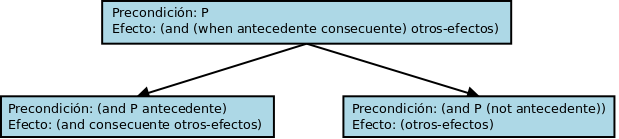
\includegraphics[width=14cm,height=3.5cm]{ef.png}
		\caption{Expansi\'on Total para Efectos Condicionales}
		\label{gbraun:compiEF}
	\end{figure}


        En este sentido, enunciamos la siguiente proposici\'on, asumiendo por
        simplificaci\'on, que aceptamos planes que preservan su
        tama\~{n}o polinomialmente.

	\begin{proposition}\label{propCLtoS}
		
	$STRIPS_{\emph{C}} \preccurlyeq^{x}_{p} STRIPS $
	
	\end{proposition} 

        \begin{proof}
        Aplicando la proposici\'on \ref{gbraun:NebelEfectos} y luego, por
        propiedad transitiva de la relaci\'on de compilabilidad,
        concluimos que $STRIPS_{\emph{C}} \preccurlyeq^{x}_{p} STRIPS $.
        \end{proof}

        Definiendo PDDL$_{\emph{C}}$ como una variante de PDDL
        con, \'unicamente, efectos condicionales y, dado que es lo
        mismo que STRIPS$_{\emph{C}}$ en t\'erminos de expresividad,
        reemplazamos en la proposici\'on anterior y obtenemos:

        \begin{corolario}
		
	$PDDL_{\emph{C}} \preccurlyeq^{x}_{p} STRIPS $
	
	\end{corolario} 

        De este resultado, concluimos que PDDL$_{\emph{C}}$ es
        \emph{compilable} a STRIPS en tiempo
        polinomial y el tama\~{n}o de los planes es
        preservado polinomialmente. 

        A continuaci\'on, vemos un ejemplo para analizar el esquema
        de traducci\'on definido en esta secci\'on y luego conclu\'imos
        sobre los supuestos de simplificaci\'on en relaci\'on al uso
        de efectos condicionales en acciones.
	 
	 \begin{ejemplo}
         
         Redefinimos la acci\'on \texttt{stack} del ``Mundo de
         Bloques'' en PDDL$_{\emph{C}}$, aplicamos 
         expansi\'on completa y mostramos los STRIPS
         equivalentes.

         \begin{verbatim}
(:action stack
   :parameters (?X ?Y ?Z)
   :precondition (and (clear ?X) (clear ?Z) (on ?X ?Y))
   :effects (and (on ?X ?Z) (clear ?Y) (not (on ?X ?Y)) 
                 (when (not (= table ?Z)) (not (clear ?Z))))
)
	\end{verbatim}

        Generamos las dos intancias de \texttt{stack} aplicando todas
        las combinaciones consistentes del antecedente del efecto condicional:

        \begin{verbatim}
(:action stack
   :parameters (?X ?Y ?Z)
   :precondition (and (clear ?X) (clear ?Z) 
                      (on ?X ?Y) (not (= table ?Z)))
   :effects (and (on ?X ?Z) (clear ?Y) 
                 (not (on ?X ?Y)) 
                 (not (clear ?Z)))
)

(:action stack1
   :parameters (?X ?Y ?Z)
   :precondition (and (clear ?X) (clear ?Z) 
                      (on ?X ?Y) (= table ?Z))
   :effects (and (on ?X ?Z) (clear ?Y) (not (on ?X ?Y)))
)
	\end{verbatim}
	 
         Finalmente, expresamos estas acciones usando notaci\'on
         STRIPS:

        \begin{verbatim}
% stack(X,Y,Z)
Precondiciones: clear(X), clear(Z), on(X,Y), Z \== table 
Borrados: on(X,Y), clear(Z)
Agregados: on(X,Z), clear(Y)

% stack1(X,Y,Z)
Precondiciones: clear(X), clear(Z), on(X,Y), Z == table 
Borrados: on(X,Y)
Agregados: on(X,Z), clear(Y)
	\end{verbatim}
	\end{ejemplo}
	
        A partir de este an\'alisis, establecemos los siguientes supuestos de
        simplificaci\'on para modelar dominios de planificaci\'on
        con efectos condicionales:

        \begin{enumerate}

        \item Los antecedentes s\'olo pueden ser de la forma: \texttt{(= X
        Y)} y \texttt{(not (= X Y))}. Esta restricci\'on se debe a que
        adem\'as de STRIPS est\'andar aceptamos el uso del predicado
        de igualdad y su negaci\'on en las precondiciones de las
        acciones.

        \item Los efectos condicionales pueden definir s\'olo un antecedente
        y s\'olo un consecuente.

        \end{enumerate}

        En base a lo expuesto, concluimos que PDDL$_{\emph{C}}$ es soportando por el
        Planificador Continuo con los supuestos establecidos previamente.

        
	 
%%%%%%%% PRECONDICIONES DISYUNTIVAS


%	\section{STRIPS$_{D}$} \label{cap5:preconddisy}

        \section{PDDL$_{D}$} \label{cap5:preconddisy}

        Las {\bf precondiciones disyuntivas} permite 
	el uso del operador \texttt{`or'} en precondiciones y
	descripciones de metas. Este operador no es soportando
        por STRIPS est\'andar y, por lo tanto, es necesario realizar un 
        prepocesamiento.

        A continuaci\'on, enunciamos y demostramos formalmente la
        relaci\'on entre STRIPS$_{D}$ y STRIPS.
	
	\begin{proposition}\label{propDtoS}
	
	$STRIPS_{D} \preccurlyeq^{1}_{p} STRIPS$
	
	\end{proposition}

        \begin{proof}
     
	En base a la proposici\'on $STRIPS_{D} \preccurlyeq^{1}_{p}
        STRIPS_{L}$, demostrada por Nebel
        en \cite{gbraun:Nebel:2001:EPP}, la proposici\'on \ref{cap5:stripsLtostrips}
	y la propiedad transitiva de la relaci\'on de compilabilidad, 
	conclu\'imos que existe un esquema de compilaci\'on de tiempo
        polinomial de $STRIPS_{D}$ a $STRIPS$ que preserva
        exactamente el tama\~{n}o del plan. El siguiente esquema de compilaci\'on ser\'ia una alternativa
        posible. 
        \ \\

        Sea $\Sigma$ un conjunto finito de \'atomos proposicionales y
        $L_{\Sigma}$ un conjunto de f\'ormulas conjuntivas compuestas por
        literales sobre $\Sigma$.
        Sea tambi\'en, $L$ un conjunto de literales y $L \subseteq \hat{\Sigma}$ donde
        $\hat{\Sigma} = \top \cup \bot \cup literales(\Sigma)$.

	Por cada operador:
        \begin{center}
	$o = \left\langle (c_{1} \vee ... \vee c_{n}),L \right\rangle$
        \end{center}

	donde $c_{i} \in L_{\Sigma}$, se generan los siguientes
        operadores:

        \begin{center}
	$o_{i} = \left\langle (c_{i}), L \right\rangle$ 
        \end{center}
        \end{proof}

        Dado que STRIPS$_{D}}$ es equivalente, en t\'erminos de
        expresividad, a PDDL con
        precondiciones disyuntivas como \'unico requerimiento, podemos
        denotar este formalismo como PDDL$_{D}$. Por lo tanto,
        concluimos el siguiente corolario:
	
        \begin{corolario}%\label{cap5:pddldstrips}
	
	$PDDL_{D} \preccurlyeq^{1}_{p} STRIPS$
	
	\end{corolario}

        Este corolario nos indica que PDDL$_{D}$ puede ser compilado a
        STRIPS en tiempo polinomial y preservando exactamente el
        tama\~{n}o de los planes.

	
        \begin{figure}[h!]
	\centering
		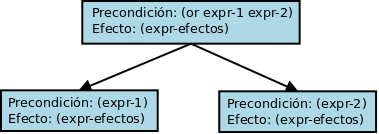
\includegraphics[width=8.5cm,height=3.5cm]{pd.png}
		\caption{Traducci\'on de Precondiciones Disyuntivas}
		\label{gbraun:predisytrad}
	\end{figure}

        Las precondiciones de las acciones que contienen disyunci\'on
	son expresadas en forma normal conjuntiva (i.e., como una
	conjunci\'on de disyunciones) y la compilaci\'on a STRIPS
	implica expresar esta precondici\'on como forma normal
	disyuntiva (i.e., como disyunci\'on de
	conjunciones). Por \'ultimo, cada subexpresi\'on de la
	disyunci\'on es la precondici\'on de una nueva acci\'on
	STRIPS como  muestra la figura \ref{gbraun:predisytrad}.
        A diferencia de los efectos condicionales, no hay un crecimiento
	exponencial de acciones dado que esta cantidad es 
        s\'olo proporcional a la cantidad de disyuntores
	en la precondicion de la acci\'on.

        El pr\'oximo ejemplo ilustra la traducci\'on propuesta:

        \begin{ejemplo}%{Traducci\'on de PDDL$_{D}$ a PDDL$_{STRIPS}$}

        La precondici\'on incluye el nuevo requerimiento \texttt{or} 
        estableciendo que un objeto, \texttt{?X}, puede ser apilado sobre
	un objeto, \texttt{?Z}, si \texttt{?Z} es la mesa (\texttt{istable}) u 
        otro bloque sin ning\'un bloque apilado.
	
	\begin{verbatim}		  
(:action stack
   :parameters (?X ?Y ?Z)
   :precondition (and (or (istable ?Z) (clear ?Z))
                      (clear ?X) (on ?X ?Y))
   :effect (and (on ?X ?Z) (clear ?Y)
                (not (clear ?Y)) (not (on ?X ?Y)))
)	
	\end{verbatim}

        Luego, la precondici\'on queda expresada de la siguiente manera:

        \begin{verbatim}		  
(:action stack
   :parameters (?X ?Y ?Z)
   :precondition (or (and (istable ?Z) (clear ?X) (on ?X ?Y))
                     (and (clear ?Z) (clear ?X) (on ?X ?Y)))
   :effect (and (on ?X ?Z) (clear ?Y)
                (not (clear ?Y)) (not (on ?X ?Y)))
)	
	\end{verbatim}
        
        El paso final del algoritmo consiste en generar una nueva
        acci\'on \texttt{stack1} con los mismos efectos que la
        acci\'on original.

        \begin{verbatim}		  
(:action stack
   :parameters (?X ?Y ?Z)
   :precondition (and (istable ?Z) (clear ?X) (on ?X ?Y))
   :effect (and (on ?X ?Z) (clear ?Y)
                (not (clear ?Y)) (not (on ?X ?Y)))
)	


(:action stack1
   :parameters (?X ?Y ?Z)
   :precondition (and (clear ?Z) (clear ?X) (on ?X ?Y))
   :effect (and (on ?X ?Z) (clear ?Y)
                (not (clear ?Y)) (not (on ?X ?Y)))
)
	\end{verbatim}

        Por \'ultimo, escribimos las acciones en notaci\'on STRIPS:

        \begin{verbatim}
% stack(X,Y,Z)
Precondiciones: istable(Z), clear(X), on(X,Y)
Borrados: clear(Y), on(X,Y)
Agregados: clear(Y), on(X,Z)		  

% stack1(X,Y,Z)
Precondiciones: clear(Z), clear(X), on(X,Y)
Borrados: clear(Y), on(X,Y)
Agregados: clear(Y), on(X,Z)		  
	\end{verbatim}
	\end{ejemplo}
	

        En base a este an\'alisis, concluimos que PDDL$_{D}$ puede ser
        traducido a STRIPS y, por lo tanto, es
        soportado por el Planificador Continuo.
	
	
%%%%%%%%% PRECONDICIONES UNIVERSALES
	

        \section{PDDL$_{\emph{u}}$} \label{cap5:precondUniv}

        Las {\bf precondiciones universales} implican el uso del
        cuantificador universal \texttt{`$\forall$'}, usualmente
        le\'ido como ``para todo''. 
        El uso de este cuantificador
        en precondiciones permite modelar acciones del mundo real como,
        por ejemplo, el comando \texttt{rmdir} de \emph{UNIX}, 
        que elimina un determinado directorio si \emph{todos} los archivos dentro
	de \'el fueron eliminados previamente.
	
        Las precondiciones universales no son soportadas en STRIPS
        est\'andar y, por lo tanto, es necesaria una traducci\'on de este
        requerimiento. El enfoque es simple. Los cuantificadores universales son 
        traducidos a una conjunci\'on de literales. Cada uno de esos literales se genera
	instanciando el par\'ametro cuantificado con cada uno
	de los objetos declarados en la definici\'on del problema de planificaci\'on.
	
	\begin{ejemplo}%{Expresiones cuantificadas universalmente}

	Sean los objetos: \texttt{block1} y \texttt{block2} y 
        supongamos la siguiente precondici\'on: \texttt{(forall (?a)
	(clear(?a)))}. Instanciando \texttt{?a} con los objetos 
	\texttt{block1} y \texttt{block2} obtenemos la precondici\'on
	equivalente: \texttt{(and (clear(block1)) (clear(block2)))}.
	
	\end{ejemplo}


        Antes de formalizar la traducci\'on de precondiciones
        universales, vamos a introducir la definici\'on de
        \emph{Base de Herbrand} extra\'ida
        de \cite{gbraun:Weld99recentadvances}:
	
%Herbrand base	
	\begin{definition} \label{def:herbrand}
	
	Sea $\Delta$ una sentencia de primer orden y libre de
        funciones. La \texttt{Base de Herbrand} $\Upsilon$
	es definida, recursivamente, de la siguiente manera:\\

		$\Upsilon (\Delta)  =  \Delta$, si $\Delta$  no
		contiene cuantificadores \\
		
		$\Upsilon (\forall_{t_{1}} x \Delta (x)) = \Upsilon
                (\Delta_{1}) \wedge ... \wedge \Upsilon (\Delta_{n})$
        \ \\

        donde $\Delta_{i}$ corresponde a cada posible interpretaci\'on
        de $\Delta(x)$ bajo el universo compuesto por los
        objetos de tipo $t_{1}$ del problema de planificaci\'on.

	\end{definition}

        Adem\'as, establecemos los siguientes supuestos de simplificaci\'on:

        \begin{enumerate}

        \item La cuantificaci\'on universal s\'olo es permitida en
        precondiciones\footnote{PDDL permite el uso de
        cuantificaci\'on universal tambi\'en en metas.}. 

        \item El mundo a modelar incluye un conjunto finito y
        est\'atico de objetos. Para el ejemplo del ``Mundo de Bloques'', la cantidad
        de \emph{bloques} debe ser finita y permanecer invariable mientras se
        planifica la soluci\'on.

        \item Todos los objetos involucrados deben ser del mismo
        tipo. Por lo tanto, no explicitamos el tipo $t_{1}$ de los objetos, tal como
        lo expresa la definici\'on \ref{def:herbrand}. 
        Continuando con el ejemplo del ``Mundo de Bloques'', los \'unicos
        objetos declarados deben ser \emph{bloques}. 

        \end{enumerate}
	
        En este sentido, estamos en condiciones de formular y
	demostrar el siguiente teorema. Sea STRIPS$_{\emph{u}}$, el formalismo
	resultante de adicionar precondiciones universales al STRIPS
	est\'andar. Entonces:

	
	\begin{teorema} \label{teorema:UP}
		
	$STRIPS_{\emph{u}} \preccurlyeq^{1}_{p} STRIPS$
	
	\end{teorema} 
	

	\begin{proof}
	Vamos a demostrar que existe una esquema de compilaci\'on de
	tiempo polinomial que preserva exactamente el tama\~{n}o de
	los planes. Por definici\'on de \emph{Base de Herbrand} y por
	los supuestos de simplificaci\'on, podemos definir el
	siguiente esquema de compilaci\'on.
        \ \\

        Sea $\Sigma$ un conjunto finito de \'atomos proposicionales y
        $L_{\Sigma}$ un conjunto de f\'ormulas conjuntivas compuestas por
        literales sobre $\Sigma$.
        Sea tambi\'en, $L$ un conjunto de literales y $L \subseteq \hat{\Sigma}$ donde
        $\hat{\Sigma} = \top \cup \bot \cup literales(\Sigma)$.
	
	Para cada operador:
	
	\begin{center}
	$o = \left\langle (\forall x_{i} (c_{j}(x_{i}))), L \right\rangle$
	\end{center}
	
	donde $c_{j}(x_{i})$ son predicados de aridad $n$ y
        $c_{j}(x_{i}) \in L_{\Sigma}$,	
	es posible generar un nuevo operador expresado como una
        conjunci\'on de literales:
	
	\begin{center}
	$o = \left\langle (c(x_{1}) \wedge ... \wedge c(x_{n})), L \right\rangle$ 
	\end{center}

        Por lo tanto, aplicando la proposici\'on
        \ref{cap5:stripsLtostrips} y luego la propiedad transitiva de
        la relaci\'on de compilabiliad, concluimos que $STRIPS_{\emph{u}} \preccurlyeq^{1}_{p} STRIPS$.
	\end{proof}

        Dado que STRIPS$_{\emph{u}}$ es equivalente, en t\'erminos de
        expresividad, a PDDL con
        precondiciones universales como \'unico requerimiento, podemos
        denotar este formalismo como PDDL$_{\emph{u}}$. Luego,
        enunciamos el siguiente corolario:

	\begin{corolario} %\label{teorema:UP}
		
	$PDDL_{\emph{u}} \preccurlyeq^{1}_{p} STRIPS$
	
	\end{corolario} 

        Este corolario nos indica que PDDL$_{\emph{u}}$
	puede ser compilado a STRIPS en tiempo polinomial y
	preservando exactamente la longitud de los planes. 
        \ \\

        Aplicamos este resultado al siguiente ejemplo:

        
        \begin{ejemplo}

        La precondici\'on para la acci\'on \texttt{stack} es que todo objeto
        en el problema debe estar sobre la mesa (\texttt{ontable})
        para que dos bloques puedan ser aplilados.
	
	Dado el siguiente problema PDDL y la
	acci\'on \texttt{stack} definida en PDDL$_{\emph{u}}$:
	
	\begin{verbatim}
(define (problem pb1)
   (:domain bkwup)
   (:objects a b c)
   (:goal (on a b))
   (:init (ontable c) (ontable b) (ontable a) 
          (on a c) (clear a)  (clear b) (armempty))
)

(:action stack
  :parameters  (?ob ?underob)
  :precondition (and (forall (?block) (ontable ?block))
                     (clear ?underob) (holding ?ob))
  :effect (and (clear ?ob) (on ?ob ?underob) (armempty)
               (not (clear ?underob)) (not (holding ?ob)))
)
	\end{verbatim}

        Aplicamos el esquema de compilaci\'on presentado y obtenemos
	la siguiente acci\'on:

	\begin{verbatim}	
(:action stack
   :parameters (?ob ?underob)
   :precondition (and (ontable a) (ontable b)(ontable c)
                      (clear ?underob)(holding ?ob)) 
   :effect (and (clear ?ob) (on ?ob ?underob) (armempty)
               (not (clear ?underob)) (not (holding ?ob)))
)
	\end{verbatim}

Finalmente, la representamos en notaci\'on STRIPS.

	\begin{verbatim}
% stack(X,Y)
Precondiciones: ontable(a), ontable(b), ontable(c), clear(Y), holding(X)
Borrados: clear(Y), holding(X)
Agregados: clear(X), on(X,Y), armempty
	\end{verbatim}
	\end{ejemplo}


	A partir de lo expuesto en esta secci\'on, podemos concluir
        que la variante PDDL$_{\emph{u}}$ es soportada por el Planificador Continuo.
        \ \\

        En este cap\'itulo hemos definido los esquemas de traducci\'on correspondientes
        para los re\-que\-ri\-mien\-tos PDDL incluidos en la
        investigaci\'on. Tales esquemas permiten traducir una
        especificaci\'on en un subconjunto de PDDL a una
        representaci\'on equivalente en la notaci\'on STRIPS soportada
        por el Planificador Continuo.

        En el pr\'oximo cap\'itulo estudiaremos la arquitectura
        propuesta para el traductor, formalizaremos el lenguaje fuente
        y destino y detallaremos aspectos
        principales de la implementaci\'on en Ciao Prolog.


 %Traduccion

\chapter{Implementaci\'on Propuesta} \label{pagcap6}


Tal como comentamos en cap\'itulo \ref{pagcap2}, la irrupci\'on de
PDDL como lenguaje est\'andar para representaci\'on de problemas de
planificaci\'on ha generado nuevos desaf\'ios. Estos desaf\'ios est\'an
motivados por la necesidad de desarrollar y/o extender herramientas que
lo soporten y tambi\'en, en ampliar su expresividad para adecuarlo a
los dominios de aplicaci\'on destino. 

Un caso puntual es el algoritmo de Planificaci\'on Continua, 
implementado por Moya en \cite{gbraun:tesisMarioMoya}, y que hemos descripto en el
cap\'itulo \ref{pagcap3}. 
En este algoritmo, que hereda algunos conceptos del pla\-ni\-fi\-ca\-dor 
POP \cite{gbraun:pop:1991}, todas las especificaciones son 
representadas usando variantes de STRIPS y, por lo tanto, es necesario
una traducci\'on para que el planificador pueda beneficiarse de las
caracter\'isticas de PDDL.

El cap\'itulo est\'a organizado de la siguiente manera. 
La secci\'on \ref{cap5:descripcionGen} presenta una descripci\'on
general de la soluci\'on, la definici\'on de los lenguajes fuente y destino
del traductor propuesto y la arquitectura dise\~{n}ada para 
su implementaci\'on. En la secci\'on \ref{cap5:Ciao}
se analizan las caracter\'isticas m\'as relevantes de Ciao Prolog
(principalmente, Expansiones Sint\'acticas y DCG) y 
se concluye acerca de su elecci\'on como entorno de 
desarrollo. Por \'ultimo, la secci\'on \ref{cap6:implementacion} detalla la implementaci\'on
del traductor y la secci\'on \ref{cap6:ejemplos} presenta algunos ejemplos de uso.


\section{Descripci\'on General de la Soluci\'on} \label{cap5:descripcionGen}

	En esta tesis proponemos el dise\~{n}o y desarrollo de un m\'odulo traductor de un 
	subconjunto de lenguaje PDDL para la especificaci\'on de
        problemas de planificaci\'on. El objetivo central es que estos
        problemas puedan ser manipulados por el Framework de Planificaci\'on Continua. 
        El traductor propuesto toma una especificaci\'on PDDL como entrada 
	y la traduce a una especificaci\'on equivalente STRIPS. La
	implementaci\'on es una expansi\'on sint\'actica para Ciao
        Prolog.

        La arquitectura inicial del traductor es ilustrada en
        la figura \ref{gbraun:traductor}.
        El m\'odulo recibe una especificaci\'on 
        en un {\bf lenguaje fuente} y retorna una especificaci\'on equivalente en un
        {\bf lenguaje destino}.


        \begin{figure}[h!]
	\centering
		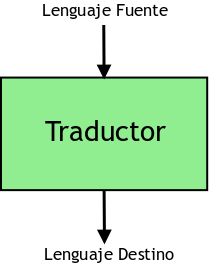
\includegraphics[width=4.5cm,height=6cm]{traductor.png}
		\caption{M\'odulo Traductor}
		\label{gbraun:traductor}
	\end{figure}

        
        A continuaci\'on, especificaremos los lenguajes fuente y
        destino y luego estudiaremos el m\'odulo traductor con m\'as detalle.

	\subsection{El Lenguaje Fuente} \label{cap6:fuente}

        El lenguaje fuente abarca los siguientes
        formalismos definidos en el cap\'itulo \ref{pagcap5}:

        \begin{itemize}

        \item PDDL$_{STRIPS}$. PDDL con el requerimiento
        \texttt{strips}. La expresividad subyacente es equivalente a STRIPS est\'andar.
        
        \item PDDL$_{L}$. PDDL con los requerimientos \texttt{strips} y \texttt{equality}.
        Tambi\'en permite la inclusi\'on de negaci\'on de igualdad en
        precondiciones. El predicado de igualdad y su negaci\'on son soportados por el
        Planificador Continuo y fueron considerados como
        parte del lenguaje fuente aunque no est\'en definidos en STRIPS est\'andar.

        \item PDDL$_{\emph{C}}$. Esta variante PDDL soporta
        \texttt{strips}, \texttt{equality} y
        \texttt{conditional-effects}. Los efectos condicionales
        est\'an restringidos a la definici\'on de un solo antecedente y
        un solo consecuente. Los antecedentes deben ser de la forma \texttt{(= X
        Y)} o \texttt{(not (= X Y))}.

        \item PDDL$_{D}$. PDDL con los requerimientos \texttt{strips},
          \texttt{equality} y \texttt{disjuntive-preconditions}.

        \item PDDL$_{u}$. PDDL con los requerimientos \texttt{strips},
        \texttt{equality} y \texttt{universal-preconditions}. Las precondiciones
        cuantificadas universalmente requieren que el problema defina por un conjunto finito y
        est\'atico de objetos. Todos estos objetos deben ser del mismo tipo.

        \end{itemize}
        
        Cada problema de planificaci\'on de entrada debe estar
        especificado en cualquiera de estos formalismos pertenecientes
        al lenguaje fuente. 

        \subsection{El Lenguaje Destino} \label{cap5:destino}

        Como parte del lenguaje destino, vamos a identificar dos
        representaciones similares. Por un lado, la notaci\'on STRIPS
        gen\'erica que ofrece el traductor y por otro, c\'omo esta
        representaci\'on es adaptada al algoritmo de Planificaci\'on
        Continua.

        El m\'odulo traductor propuesto ofrece una notaci\'on
        gen\'erica que permite personalizar la definici\'on de STRIPS
        seg\'un el algoritmo planificador al que se quiera
        integrar dicho m\'odulo. Esta representaci\'on
        permite reutilizar el traductor en otros
        algoritmos, cuyo lenguaje de representaci\'on sea similar a STRIPS,
        sin la necesidad de modificar los m\'odulos principales de traducci\'on.
        La notaci\'on gen\'erica definida, llamada 
        \emph{Prolog-like}, es la siguiente:


        \begin{itemize}

        \item \emph{Precondiciones, Agregados y Borrados}. Por cada acci\'on en el dominio de
        entrada, el traductor genera los predicados \texttt{preconditions}, \texttt{achieves}
        y \texttt{deletes} respectivamente, con los siguientes
        argumentos: \texttt{action\_name(parameters)} y una lista de
        predicados \texttt{[pre\-di\-ca\-te$_{1}$(pa\-ra\-men\-ters$_{1}$),...,
        predicate$_{N}$(paramenters$_{N}$)]}, donde \texttt{parameters$_{i}$} es
        una lista de variables Prolog separada por comas. 

        \item \emph{Objetos, Meta y Estado Inicial}. El traductor genera un
        predicado \texttt{objects(obj$_{1}$,obj$_{2}$,...,obj$_{N}$)}
        donde \texttt{obj$_{i}$} es un \'atomo
        Prolog. Adem\'as, genera \texttt{goal(fact$_{g}$)} donde \texttt{fact$_{g}$} son
        hechos Prolog de la forma \texttt{fact(parameters$_{g}$)} y 
        \texttt{parameters$_{g}$} es una lista de \'atomos separados
        por comas. Por \'ultimo,
        \texttt{init(fact$_{1}$,fact$_{2}$,..,fact$_{N}$)} es la
        definici\'on del estado inicial
        donde, \texttt{fact$_{i}$} es de la
        forma \texttt{init(parameters$_{i}$)}
        y \texttt{parameters$_{i}$} es una lista de \'atomos separados
        por comas. 
 
        \end{itemize}

        A continuaci\'on, mostramos un ejemplo con la notaci\'on
        gen\'erica definida para el traductor.

        \begin{ejemplo}
        \begin{verbatim}
% Dominio	
preconditions(action_name_1(parameters), 
         [predicate_1(paramenters_1), 
         ...
         predicate_N(paramenters_N)]).   
achieves(action_name_1(parameters),
         [predicate_1(paramenters_1),
         ...
         predicate_N(paramenters_N)]).
deletes(action_name_1(parameters),
         [predicate_1(paramenters_1),
         ...
         predicate_N(paramenters_N)]).

% Problema
(domain(domain_name),
 objects(obj1,obj2,..,objN),
 goal(fact_g),
 init(fact_1,fact_2,..,fact_N)).
        \end{verbatim}
        \end{ejemplo}

        Teniendo en cuenta que uno de los objetivos de nuestra investigaci\'on es
        integrar el m\'odulo al Framework de Planificaci\'on
        Continua, el lenguaje destino del traductor est\'a restringido al lenguaje
        de representaci\'on soportado por el algoritmo de
        planificaci\'on que implementa el framework.
        En este caso, los dominios y problemas de planificaci\'on est\'an
        especificados en STRIPS est\'andar m\'as los predicados
        de igualdad (denotado como \texttt{`=='}) y distinto (denotado
        como \texttt{`\textbackslash =='}).
        Cada acci\'on se compone de un
        predicado \texttt{preconditions}, un nuevo
        predicado \texttt{deletes} por cada predicado en
        la lista de borrados gen\'erica y un predicado \texttt{achieves}
        por cada predicado en la lista gen\'erica de
        agregados.
        Para adaptar los problemas, la traducci\'on es similar. Por cada
        predicado gen\'erico en \texttt{init} se genera un nuevo hecho
        Prolog con la sintaxis \texttt{holds(fact$_{i}$,init)}. 

        Luego, la representaci\'on Ciao Prolog lograda es la siguiente:

        \begin{verbatim}
% action(X,Y,Z)
preconditions(action(X,Y,Z),[pred1(X),pred2(Y),pred3(Z)]):- X == Y,Y \== Z.
achieves(action(X,Y,Z),pred1(X)).
achieves(action(X,Y,Z),pred3(Z)).
deletes(action(X,Y,Z),pred2(Y)).

% Problem
holds(pred1(object1),init).
holds(pred2(object2),init).
holds(pred3,init).
        \end{verbatim}  
        

        A continuaci\'on, detallaremos la
        arquitectura del traductor y analizaremos el comportamiento de
        cada uno de sus m\'odulos.


	\subsection{M\'odulos de la Arquitectura} \label{cap5:modarq}
	
	La arquitectura del traductor est\'a organizada en los
        siguientes m\'odulos:
	
	\begin{itemize}
	
	\item \texttt{pddltostrips}: es el m\'odulo
	``controlador'' y debe incluirse en la especificaci\'on PDDL de entrada
	usando la sentencia Prolog
        \texttt{use\_package(pddltostrips)}. Permite cargar el 
        m\'odulo \texttt{pddltostrips\_tr} y el
	predicado \texttt{parser\_ext} en tiempo de compilaci\'on
        para comenzar la traducci\'on.
	
	
	\item \texttt{pddltostrips\_tr}: este m\'odulo incluye la
        definici\'on del predicado \texttt{parser\_ext}. 
        El pre\-di\-ca\-do recibe un dominio y un problema en PDDL y retorna
        la especificaci\'on STRIPS correspondiente. Interact\'ua con
        los m\'odulos \texttt{tokenizer}, \texttt{parse\_problem}
        y \texttt{parse\_domain}. 
        Este m\'odulo tambi\'en es el que interpreta la
        representaci\'on gen\'erica STRIPS para adaptar el traductor
        al planificador destino.
	
	\item \texttt{pddl\_domain}: usando el paquete \texttt{dcg}, traduce la definici\'on de un
        dominio PDDL, expresado en el lenguaje fuente, a una lista de predicados 
	Prolog en la notaci\'on STRIPS gen\'erica definida en la
        secci\'on anterior. El predicado principal de este m\'odulo es \texttt{parse\_domain}.
	
	\item \texttt{pddl\_problem}: usando el paquete \texttt{dcg}, traduce la definici\'on de un
	problema PDDL, expresado en el lenguaje fuente, a una lista de predicados
	Prolog en la notaci\'on STRIPS gen\'erica definida. El
	predicado principal de este m\'odulo es \texttt{parse\_problem}.
	
	\item \texttt{tokenizer}: este m\'odulo act\'ua como
	analizador l\'exico\footnote{Un analizador l\'exico lee una
	cadena de caracteres de la especificaci\'on en el lenguaje
	fuente y los agrupa en secuencias
	llamadas \emph{lexemas}. Para cada \emph{lexema}, el
	analizador genera un \emph{token} como salida \cite{gbraun:Aho:2007}.} y 
        obtiene los \emph{tokens} de la definici\'on PDDL de entrada.
	
	\end{itemize}
	
	Para utilizar este m\'odulo traductor, la especificaci\'on
	PDDL de entrada debe ser importada desde el planificador destino. 
	Esta especificaci\'on, a su vez, debe importar el
	paquete \texttt{pddltostrips} implementado.
        El am\-bien\-te provisto por Ciao Prolog generar\'a, en compilaci\'on, los
	STRIPS equivalentes y el planificador
	podr\'a hacer uso de ellos para producir un plan.
	La figura \ref{pddl:modules} ilustra la disposici\'on e
        interacci\'on de los m\'odulos mencionados\footnote{Las
        l\'ineas puntuadas entre los m\'odulos representan la
        dependencia entre ellos.}.  
	
	\begin{figure}
	\centering
		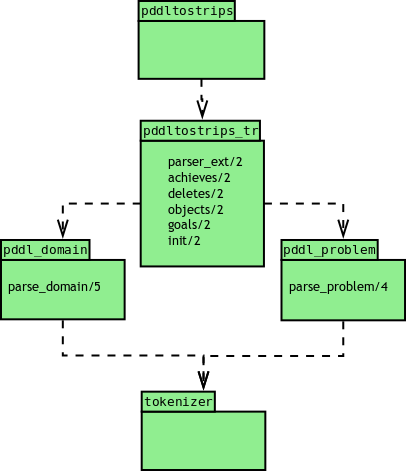
\includegraphics[width=8cm,height=9cm]{UMLParser.png} 
		\caption{Arquitectura Modular del Traductor}
		\label{pddl:modules}
	\end{figure}

        En la secci\'on siguiente analizaremos y
        justificaremos la elecci\'on de Ciao Prolog como el am\-bien\-te
        de programaci\'on ideal para la implementaci\'on del
        traductor PDDL. Tambi\'en, discutiremos brevemente, la noci\'on de expansiones
        sint\'acticas y, en particular, la expansi\'on DCG.

        \section{Ciao Prolog} \label{cap5:Ciao}

	El sistema Ciao \cite{ciao-reference-manual-tr} es un ambiente
        de programaci\'on para el desarrollo de aplicaciones en
        lenguaje Prolog \cite{shapiro:1997:APA:6686} y en varios otros 
        lenguajes que son extensiones y modificaciones de Prolog. 
        Un aspecto importante de Ciao es que, adem\'as de dar soporte 
        para la programaci\'on l\'ogica, prove\'e al programador de un 
        conjunto de caracter\'isticas de diferentes paradigmas y
        estilos de programaci\'on que 
	pueden ser inclu\'idas en cada m\'odulo de un programa. 
        El lenguaje est\'a dise\~{n}ado para ser 
	extendido de una manera simple y modular.
	
	Ciao Prolog presenta el siguiente conjunto de caracter\'isticas:
	
	\begin{itemize}
	
	\item Ofrece un sistema Prolog completo, soportando 
        ISO-Prolog\footnote{International Standard ISO/IEC
        13211-1} \cite{gbraun:estandarprolog}, 
        que permite tanto res\-trin\-gir como expandir el lenguaje
        mediante un sistema modular novedoso.
	
	\item Soporta, a trav\'es de expansiones, programaci\'on
        funcional, restricciones, objetos, registros, 
	persistencia, reglas de control (\emph{breadth-first search}, 
        \emph{iterative deepening}, etc.), concurrencia, 
	ejecuci\'on distribuida y paralela. 
        Tambi\'en incluye librer\'ias para programaci\'on Web (por
        ejemplo, paquetes para manipular lenguaje html, xml, entre otros), sockets e 
	interfaces externas (C, JAVA, Bases de Datos Relacionales, etc.).
	
	\item Ofrece un soporte para programaci\'on a gran escala 
        con un sistema robusto de m\'odulos, compilaci\'on incremental,
        un lenguaje de aserciones para la declaraci\'on de propiedades de programas, 
	inferencia est\'atica y comprobaci\'on est\'atica/din\'amica de tales aserciones.
	
	\item Su compilador genera varias formas de ejecutables 
        \emph{stand-alone}\footnote{Un programa stand-alone
	 es uno que puede ejecutarse como un proceso separado.} e 
         independientes de la arquitectura. 
	 Los m\'odulos de las librer\'ias pueden ser compilados 
         como \emph{bytecode} o como compactos archivos fuentes C y 
         ligados de manera est\'atica, din\'amica o 
	 cargados autom\'aticamente. 
	
	\item Finalmente, es distribuido bajo LGPL 
        GNU\footnote{\emph{Lesser GNU General Public License}.} \cite{gbraun:lgpl}.
	
	\end{itemize}
	
	Ciao es desarrollado por el grupo CLIP de la Universidad
	Polit\'ecnica de Madrid\footnote{CLIP
          Group. \url{http://clip.dia.fi.upm.es/index.html}. Disponible
        en Septiembre de 2012.}.

	
	\subsection{Expansiones Sint\'acticas}
	
	El enfoque orientado a extensibilidad de Ciao posibilita 
	la expansi\'on del lenguaje tanto sint\'actica como
        sem\'anticamente. Estas expansiones pueden ser 
	referenciadas en los m\'odulos, sin interferir con otros,
        gracias a la noci\'on de ``paquetes'' (\emph{packages}).
	
	Una {\bf expansi\'on sint\'actica} \cite{gbraun:exp:sint:2000} 
        toma como entrada una especificaci\'on
        con una determinada sintaxis, posiblemente diferente 
	a la que permite Prolog, y genera una nueva representaci\'on, equivalente 
        a su entrada, que puede ser interpretada en Prolog.
	
	En Ciao, este procesamiento es soportado
        por la directiva \texttt{load\_com\-pi\-la\-tion\_mo\-du\-le/1}. 
	Esta directiva permite separar el c\'odigo que ser\'a usado en tiempo de
        compilaci\'on del c\'odigo que ser\'a usado en tiempo de 
	ejecuci\'on. De esta manera, permite cargar ``en el compilador'', el m\'odulo 
        especificado en su argumento.
	
	Para facilitar la definici\'on de expansiones, Ciao tambi\'en incluye
        cuatro directivas m\'as espec\'ificas. 
	El compilador invoca estos
        predicados en el momento apropiado e 
	instancian su primer argumento con los items a ser
        traducidos. Si el predicado es de aridad 3, 
	el tercer argumento opcional es instanciado con el nombre del 
        m\'odulo donde la traducci\'on se est\'a 
	llevando a cabo (algunas veces necesario durante ciertas
        expansiones). Si la llamada al predicado 
	de expansi\'on es exitosa, el t\'ermino retornado en el
        segundo argumento es usado para reemplazar al original. 
	
	En \cite{gbraun:exp:sint:2000}, Daniel Cabeza y Manuel Hermenegildo, definen las
        siguientes directivas de traducci\'on:
	
	\begin{itemize}
	
	\item \texttt{add\_sentence\_trans/1}: define la traducci\'on
        de t\'erminos, le\'idos por el compilador, 
	en el resto de la entrada actual. 
        Para cada t\'ermino subsecuente, el predicado es nuevamente 
	invocado para obtener un nuevo t\'ermino que ser\'a usado en
        lugar del t\'ermino actual. Un ejemplo 
	de este tipo de traducci\'on es el DCG (\emph{Definite Clause Grammar}).
	
	\item \texttt{add\_term\_trans/1}: define la traducci\'on de
        t\'erminos y subt\'erminos, le\'idos por el compilador, 
	en la entrada actual. Para cada t\'ermino subsecuente, y
        recursivamente, para cada subt\'ermino inclu\'ido, 
	el predicado de traducci\'on es invocado para obtener un nuevo
        t\'ermino en reemplazo del anterior. 
	Esta traducci\'on comienza luego de que todas las traducciones 
        definidas en \texttt{add\_sentence\_trans/1} son ejecutadas.
	
	\item \texttt{add\_goal\_trans/1}: define la traducci\'on de 
        las metas presentes en las cl\'ausulas de la entrada actual. 
	Esta traducci\'on comienza luego de que todas las definidas 
        en \texttt{add\_sentence\_trans/1} y 
	\texttt{add\_term\_trans/1} son ejecutadas.
	
	\item \texttt{add\_clause\_trans/1}: define la traducci\'on de
        las cl\'ausulas de la entrada actual. La traducci\'on 
	comienza antes de \texttt{add\_goal\_trans/1} pero luego de
        las traducciones \texttt{add\_sentence\_trans/1} 
	y \texttt{add\_term\_trans/1}.
	
	\end{itemize}
	
	A continuaci\'on, y en el contexto de estas directivas, podemos analizar el
        m\'odulo \texttt{pddltostrips.pl} de la implementaci\'on propuesta:
	
	\begin{verbatim}
	:- package(pddltostrips). 
	:- load_compilation_module('pddltostrips_tr'). 
	:- add_sentence_trans(parser_ext/2).
	\end{verbatim}


	La primer declaraci\'on indica que \texttt{pddltostrips} es un
        paquete. La directiva 
	\texttt{load\_com\-pi\-la\-tion\_mo\-du\-le} carga, en el compilador, el 
        c\'odigo definido en \texttt{pddltostrips\_tr}. 
	Por \'ultimo, la declaraci\'on \texttt{add\_sen\-ten\-ce\_trans\-(par\-ser\_ext/2)} invoca al predicado 
	\texttt{parser\_ext/2} exportado por \texttt{pddltostrips\_tr}. 
	El predicado realiza la traducci\'on correspondiente en tiempo de compilaci\'on.
	
		
	\subsection{Definite Clause Grammar (DCG)}
	
	La librer\'ia DCG\footnote{Definite Clause Grammars.} es una expansi\'on sint\'actica 
	para las gram\'aticas libres de contexto. Prove\'e a Prolog de
	una notaci\'on conveniente para definir estas gram\'aticas. 
	Las reglas gramaticales son un \emph{syntactic sugar} 
	para cl\'ausulas Prolog ordinarias. Cada regla toma una cadena
	de entrada, analiza alguna subcadena 
	inicial y produce la subcadena restante como salida para un
	posterior an\'alisis. Los argumentos requeridos 
	para las cadenas de entrada y salida no son indicados
	expl\'icitamente en la regla gramatical ya que la sintaxis las define impl\'icitamente.
	
	Una regla DCG en Prolog tiene la siguiente forma:
	
	\begin{verbatim}
	head --> body
	\end{verbatim}
	
	Esto significa que una forma posible para \texttt{head}
        es \texttt{body}. Ambos son secuencias de uno o m\'as \'items 
	ligados por el operador de conjunci\'on est\'andar de Prolog,
        notado como \texttt{`,'}.
	
	La gram\'aticas libres de contexto son extendidas, usando DCG,
	de la siguiente manera:
	
	\begin{enumerate}
	
	\item Un s\'imbolo no terminal puede ser cualquier t\'ermino Prolog.
	
	\item Un s\'imbolo terminal puede ser cualquier t\'ermino
        Prolog. Los s\'imbolos terminales son escritos como 
	listas Prolog y la lista vac\'ia \texttt{[ ]} representa una secuencia vac\'ia de terminales. 
	Si los terminales son caracteres ASCII, los s\'imbolos son escritos como cadenas.
	
	\item Las condiciones extras pueden ser incluidas en el \texttt{body} de la regla gramatical. 
	Las invocaciones se explicitan entre \texttt{\{ \}}.
	
	\item El \texttt{head} de la regla consiste de s\'imbolos no
        terminales. Opcionalmente, puede estar 
	con\-ti\-nua\-do por terminales (en forma de listas).
	
	\item Las alternativas puede definirse en el \texttt{body} 
        utilizando el operador \texttt{`;'}.
	
	\item El s\'imbolo de \emph{cut}, \texttt{`!'}, puede ser 
        incluido en el \texttt{body} de la regla. 
	No es necesario utilizar \texttt{\{ \}}.
	
	\end{enumerate}

        Ilustramos el uso de las DCG con el siguiente ejemplo:
	
        \begin{ejemplo}
        Extraemos el predicado \texttt{pddl2stripsdomain} implementado en el
        m\'odulo \texttt{pddl\_domain} de nuestro traductor.

	\begin{verbatim}
pddl2stripsdomain(Objs,Preconditions, Achieves, Deletes) --> 
  ['(', 'define', '(', 'domain'], name(_Name_Domain),!, [')'], 
  ((requirements_def(Reqs), {_Requirements =..[requirements|Reqs]}) | []),!, 
  ((predicates_def(Dict,Preds), {_Predicates =..[predicates|Preds]}) | []),!, 
  ((constants_def(Consts), {_Constants =..[constants|Consts]}) |[]),!,
  (actions_def(Dict,Objs,Preconditions, Achieves, Deletes) | []),!,
  [')'].
	\end{verbatim}

	Este predicado es invocado desde:
	
	\begin{verbatim}
parse_domain(Input,Objs,Preconditions,Achieves,Deletes)
	\end{verbatim}
	
	Como resultado, retorna las listas
        \texttt{Precondiciones}, \texttt{Agregados} y \texttt{Borrados} 
	co\-rres\-pon\-dien\-tes a la entrada PDDL en el argumento \texttt{Input}.
	\end{ejemplo}
	
        Hasta aqu\'i, hemos presentado los conceptos principales que soportan la
        implementaci\'on de nuestro traductor. Estamos en condiciones
        de analizar paso a paso, a partir de la pr\'oxima secci\'on, la
        implementaci\'on propuesta.

\section{Implementaci\'on del Traductor} \label{cap6:implementacion}

La traducci\'on comienza cuando se invoca, en tiempo de compilaci\'on, 
al predicado \texttt{parser\_ext/2}, cuyo c\'odigo es presentado a
continuaci\'on:

        \begin{verbatim}
parser_ext((Problem,Domain),STRIPS_POP):-
     atom_codes(Problem,CH),
     atom_codes(Domain,CH2),
     tokenizer(CH,TokensProblem),
     tokenizer(CH2,TokensDomain),
     parse_problem(TokensProblem,Objects,Goals,Init),
        
     % Problem customizable predicates to the target planner
     objects_pop(Objects,OBJ_POP),
     goals_pop(Goals,GOALS_POP),
     init_pop(Init,INIT_POP),
     append(OBJ_POP,GOALS_POP,PBL),
     append(INIT_POP,PBL,Problem),

     parse_domain(TokensDomain,OBJ_POP,Preconditions,Achieves,Deletes),

     % Domain customizable predicates to the target planner
     achieves_pop(Achieves,ACHIEVES_POP),
     deletes_pop(Deletes,DELETES_POP),
     append(ACHIEVES_POP,DELETES_POP,D1),
     append(Preconditions,D1,Domain),
     append(Domain,Problem,STRIPS_POP).
        \end{verbatim}


Este predicado recibe como entrada el par \texttt{(Domain,Problem)}
donde \texttt{Domain} y \texttt{Problem} son cadenas de caracteres
escritos como \'atomos Prolog\footnote{Atomos Prolog son cadenas de
caracteres escritos entre comas simples.}.
El predicado Ciao \texttt{atom\_codes} toma estos \'atomos y retorna
la lista de c\'odigos ASCII correspondientes. Ambos, dominio y problema 
PDDL, est\'an en listas separadas de c\'odigos. 

El pr\'oximo paso es generar, a partir de estas listas, secuencias 
significativas del lenguaje PDDL. El predicado
\texttt{tokenizer} implementa esta conducta realizando las siguientes
acciones. Por cada conducta mostramos el fragmento de c\'odigo 
correspondiente.

\begin{itemize}

\item Remueve espacios, saltos de l\'inea y tabulaciones de la lista de
c\'odigos ASCII.

          \begin{verbatim}
%layout spaces,newlines,tabs...
tokenizer([C|RC],Words):- ( C=32 ; C=10 ; C=9 ; C=13 ; C=92 ), !, 
                          tokenizer(RC,Words).
          \end{verbatim}

\item Trata como palabras a los siguientes s\'imbolos:
par\'entesis \texttt{( )}, coma \texttt{`,'}, 
punto \texttt{`.'}, gui\'on medio \texttt{`-'}, dos puntos \texttt{`:'} y al
signo de interrogaci\'on \texttt{`?'}.

         \begin{verbatim}
% Brackets, comma, period or question marks are treated as separed words
tokenizer([C|RC], [Char|Words_1]) :- ( C=40 ; C=41 ; C=44 ; C=45 ;
                                       C=46 ; C=63 ; C=58 ) , 
                                     name(Char, [C]), !,
                                     tokenizer(RC, Words_1).
         \end{verbatim}

\item El resto de los caracteres son retornados como \emph{lexemas}. 
En PDDL estos lexemas son nombres de variables y predicados, palabras
reservadas, constantes y el operador de igualdad \texttt{`='} y
negaci\'on \texttt{not}.

         \begin{verbatim}
% Words
tokenizer([C|RC], [Word|Words_1]):- word([C|RC],Chars,Next), 
                                    name(Word,Chars), 
                                    tokenizer(Next,Words_1).

word([C|RC],[],[C|RC]):- ( C=32 ; C=44 ; C=10 ; C=9 ; C=13 ; C=46 ; 
                           C=63 ; C=40 ; C=41 ; C=58 ; C= -1 ) , !.

word([C|RC],[LC|Chars],Next):- lower_case(C,LC), 
                               word(RC,Chars,Next).
         \end{verbatim} 

\end{itemize}

%tabla de caracteres ASCII para estas listas

En este instante de la traducci\'on tenemos la entrada PDDL reducida 
a listas que ser\'an interpretadas por
las gr\'amaticas definidas en los m\'odulos \texttt{pddl\_problem}
y \texttt{pddl\_domain}.

% PROBLEMAS!

El predicado \texttt{parse\_problem/4} implementado en el
m\'odulo \texttt{pddl\_problem} comienza la traducci\'on del problema
PDDL. Este predicado recibe la lista de \emph{tokens} retornadas por el 
\texttt{tokenizer} y retorna el problema PDDL expresado en la
notaci\'on Prolog gen\'erica definida en la
secci\'on \ref{cap5:destino}. 
La regla principal es analizada a continuaci\'on:

   \begin{verbatim}
pddl2stripsproblem(Objects, Goals, Init) --> 
    ['(', 'define', '(', 'problem'], name(_Name_Problem),!, [')'],
    ['(', ':', 'domain'], name(_Name_Domain), !, [')'], 
    ((objects_def(Objs), {Objects =..[objects|Objs]}) | []),!,  
    ((goals_def(Goal,_,_), {Goals =..[goal|Goal]}) | []),!, 
    ((init_def(Ini), {Init =..[init|Ini]}) | []),!, 
    [')'].
   \end{verbatim}

\texttt{pddl2stripsproblem} retorna los predicados correspondientes a
los objetos, la meta y el estado inicial del problema PDDL. Cada una
de estas secciones es analizada, respectivamente por las siguentes
reglas invocadas: \texttt{objects\_def}, \texttt{goal\_def} e \texttt{init\_def}.

El pr\'oximo paso del traductor es analizar el dominio PDDL, por lo tanto, el
predicado \texttt{parse\_domain/5} es invocado
desde \texttt{parser\_ext} para comenzar la traducci\'on. 
Recibe, como entrada, la lista de \emph{tokens} del dominio PDDL y los
objetos definidos en el problema y 
retorna tres listas: \texttt{Preconditions}, \texttt{Achieves} y \texttt{Deletes}.

La regla principal en este caso es la siguiente:

   \begin{verbatim}
pddl2stripsdomain(Objs,Preconditions, Achieves, Deletes) --> 
    ['(', 'define', '(', 'domain'], name(_Name_Domain),!, [')'], 
    ((requirements_def(Reqs), {_Requirements =..[requirements|Reqs]}) | []),!, 
    ((predicates_def(Dict,Preds), {_Predicates =..[predicates|Preds]}) | []),!, 
    ((constants_def(Consts), {_Constants =..[constants|Consts]}) |[]),!,
    (actions_def(Dict,Objs,Preconditions, Achieves, Deletes) | []),!,
    [')'].
   \end{verbatim}

Cada una de las secciones en la especificaci\'on del dominio PDDL es
analizada por las si\-guien\-tes
reglas: \texttt{requirements\_def}, \texttt{predicates\_def},
\texttt{constants\_def} y \texttt{actions\_def}.

Vamos a estudiar puntualmente la regla \texttt{actions\_def} debido a
que es la que genera las listas STRIPS. El par\'ametro \texttt{Objs}
es la lista de objetos definidos en el problema de planificaci\'on
y \texttt{Dict} es un diccionario de variables, donde cada elemento
del diccionario es un par \texttt{(PDDL
Parameter,Prolog Variable)} para gestionar la correspondencia de
nombres de par\'ametros en predicados. 

El fragmento de c\'odigo para \texttt{actions\_def} es el mostrado a
continuaci\'on.
\ \\

\ \\

        \begin{verbatim}
actions_def(Dict,Objs,Preconditions,Achieves,Deletes) --> 
      ['(',':','action'],name(Name),!, 

      [':', 'parameters'], 
      ['('], list_parameters(Dict,Param),!, [')'],
      {nth(1, Name, Name_Ac),  Ac =..[Name_Ac|Param]},

      [':', 'precondition'], 
      ['('], list_preconditions(Dict,Objs,P),
      {Pre =..[preconditions|[Ac,P]]},!, [')'],
 
      [':', 'effect'], 
      ['('], list_effects(Dict,A, D, P),
      {Ach =..[achieves|[Ac,A]],Del =..[deletes|[Ac,D]]},!, [')'], [')'],

      actions_def(Dict,Objs,PRE2,ACH2,DEL2),!,
      {((instances(P,_),append([Pre],PRE2,Preconditions),
         append([Ach],ACH2,Achieves),append([Del],DEL2,Deletes));
        (generateInstances(Pre,Ach,Del,PRE1,ACH1,DEL1),
         append(PRE1,PRE2,Preconditions),append(ACH1,ACH2,Achieves), 
         append(DEL1,DEL2,Deletes)))}.
        \end{verbatim}


En primer lugar, la regla identifica el nombre de la acci\'on 
mediante el predicado \texttt{name} y pos\-te\-rior\-men\-te,
retorna la lista de par\'ametros declarados para la acci\'on. 
Esta lista es generada desde \texttt{list\_parameters}. 
La regla \texttt{list\_preconditions} inicia la traducci\'on de las
precondiciones de la acci\'on y retorna todos los predicados definidos
para dicha acci\'on. Por \'ultimo, \texttt{list\_effects} retorna los predicados
correspondientes a las listas de agregados y borrados. 
Los efectos negados van a la lista de
borrados y el resto a la de agregados.

Finalmente, el control de la traducci\'on vuelve a \texttt{parser\_ext}. 
En este punto, el traductor permite procesar las estructuras
gen\'ericas definidas para los problemas y los dominios con el
objetivo principal de generar la notaci\'on STRIPS adecuada para el
planificador \emph{target}.
La manipulaci\'on de esta notaci\'on permite el reuso del traductor
sobre diferentes planificadores que utilicen una representaci\'on
similar a STRIPS como lenguaje de representaci\'on.
\ \\

Luego de analizar los fragmentos m\'as importantes de la
implementaci\'on del traductor, en la pr\'oxima secci\'on, vamos a
mostrar c\'omo generar la especificaci\'on PDDL de entrada en Ciao Prolog, c\'omo
invocar el traductor y algunos ejemplos de planificaci\'on utilizando
el algoritmo POP y distintas instancias del ``Mundo de Bloques''. 

   \section{Demostraci\'on del Traductor} \label{cap6:ejemplos}

   Sea el estado inicial para una instancia del ``Mundo de
   Bloques'' tal como indica la figura \ref{demo:estadoInicial}, y la
   meta, como se muestra en la figura \ref{demo:estadoFinal}.

  \begin{figure}[h!]
  \centering
  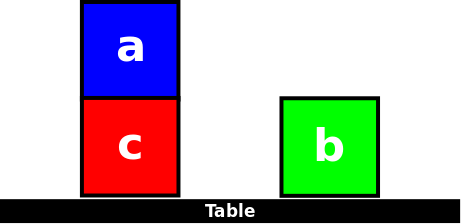
\includegraphics[width=10cm,height=4cm]{bkwInicial.png} 
       \caption{Estado Inicial del ``Mundo de Bloques''}
	\label{demo:estadoInicial}
   \end{figure} 

  \begin{figure}[h!]
  \centering
  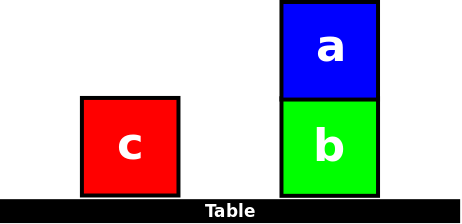
\includegraphics[width=10cm,height=4cm]{bkwFinal.png} 
       \caption{Estado Final del ``Mundo de Bloques''}
	\label{demo:estadoFinal}
  \end{figure}  

  En primer lugar, creamos un archivo llamado \texttt{bkw.pl} y
  definimos el problema y el dominio para esta instancia del ``Mundo de Bloques'' 
  como indica la pr\'oxima figura \ref{demo:pddl}. En esta definici\'on
  incluimos el paquete traductor
  mediante la cl\'ausula Prolog:

  \begin{verbatim}
  :- use_package(pddltostrips.pl).
  \end{verbatim}

  \begin{figure}[h!]
  \centering
  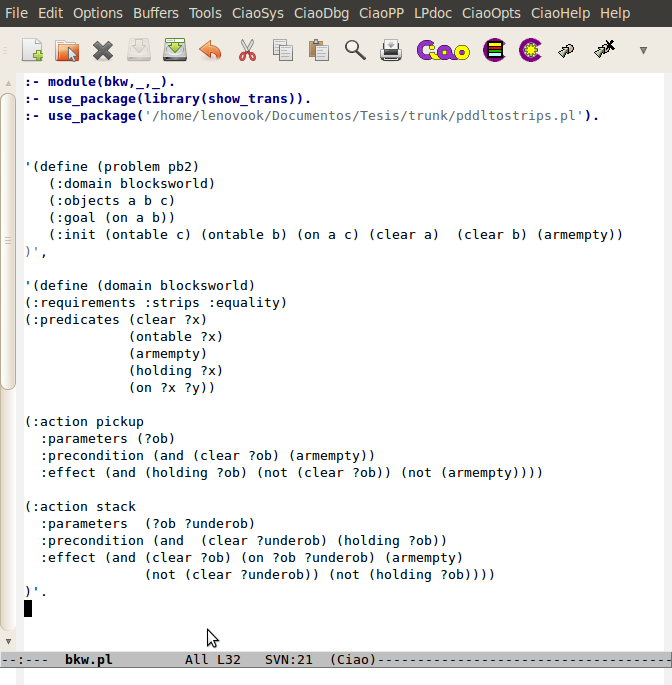
\includegraphics[width=12cm,height=9.5cm]{demoPddlCiao.png} 
       \caption{Especificaci\'on PDDL en Ciao Prolog}
	\label{demo:pddl}
   \end{figure} 

   Luego, desde el planificador (en este caso el POP), referenciamos la especificaci\'on
   PDDL anterior que ser\'a utilizada por el algoritmo
   planificador. Incluimos esta especificaci\'on usando la siguiente
   cl\'ausula, como indica la figura \ref{demo:pop}. 
   
   \begin{verbatim}
   :- use_module(`bkw',[achieves/2,preconditions/2,deletes/2,holds/2]).
   \end{verbatim}   

  \begin{figure}[h!]
  \centering
  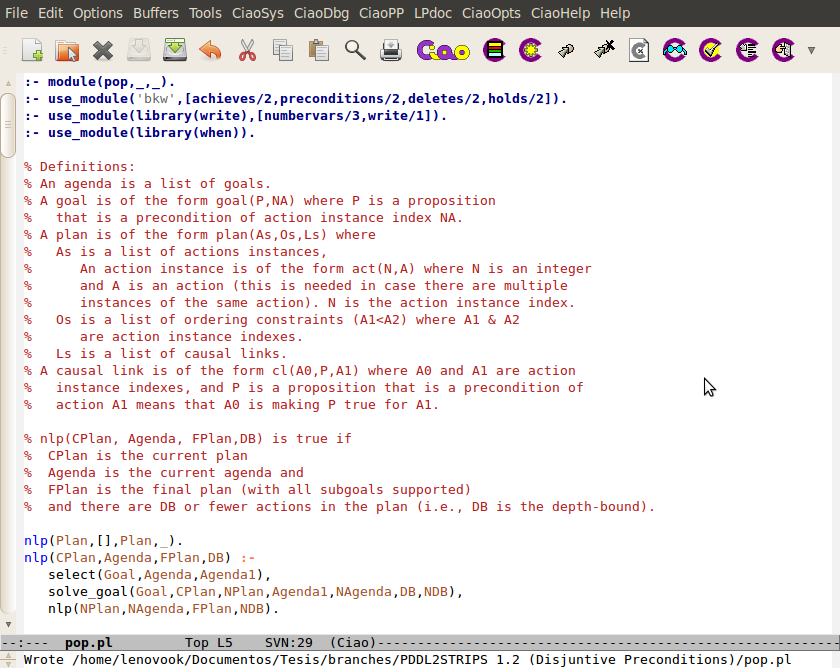
\includegraphics[width=12cm,height=9.5cm]{demoPOP.png} 
       \caption{Planificador POP en Ciao Prolog}
	\label{demo:pop}
   \end{figure}     

   Compilamos y consultamos al planificador con la siguiente
   \emph{query}: \texttt{solve([on(a,b)],P,2), seq(P,S).} para obtener
   un plan.
   Notar que la figura \ref{demo:query} tambi\'en muestra la salida
   del traductor con los STRIPS equivalentes a la especificaci\'on
   PDDL de entrada.

%   \pagebreak

  \begin{figure}[h!]
  \centering
  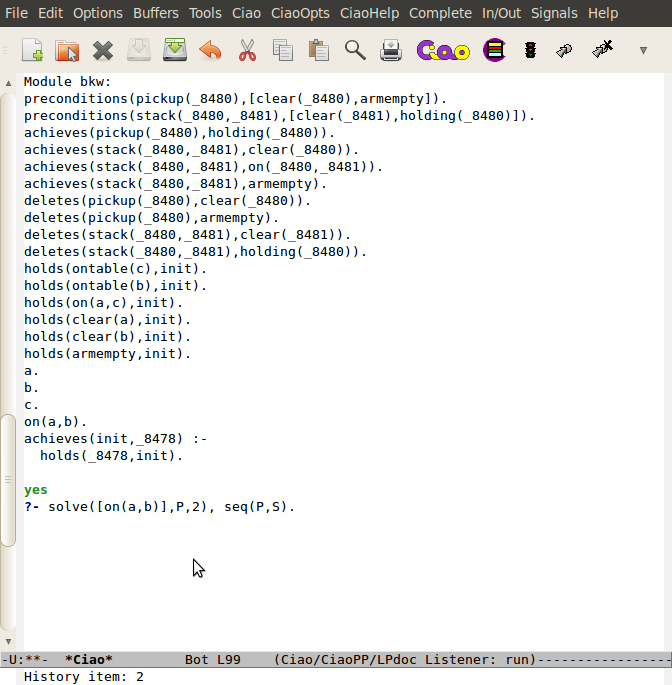
\includegraphics[width=12cm,height=9.5cm]{demoShowtransQuery.png} 
       \caption{Consulta para el planificador POP}
	\label{demo:query}
   \end{figure}

   Por \'ultimo, el planificador retorna el plan deseado que incluye las
   siguientes acciones, como tambi\'en ilustra la figura \ref{demo:plan}:
   \texttt{init, pickup(a), stack(a,b), end}.

  \begin{figure}[h!]
  \centering
  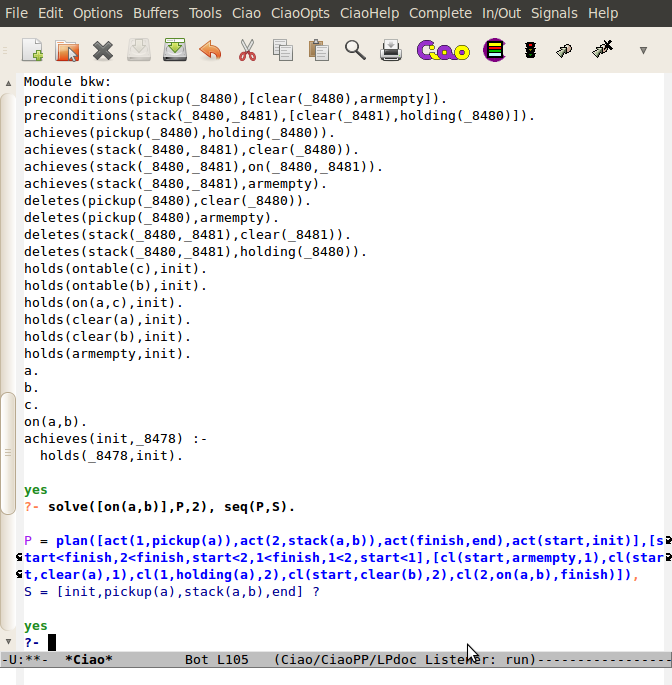
\includegraphics[width=12cm,height=9.5cm]{demoPopPlan.png} 
       \caption{Resultado obtenido de la planificaci\'on}
	\label{demo:plan}
   \end{figure}


   En este cap\'itulo hemos analizado el traductor
   propuesto, definimos su arquitectura y estudiamos el c\'odigo de la
   implementaci\'on. Tambi\'en vimos c\'omo invocar este paquete desde
   Ciao Prolog y c\'omo el traductor es integrado a un planificador
   para poder obtener un plan dada una representaci\'on inicial en
   PDDL.

   En el pr\'oximo cap\'itulo abordamos las conclusiones de esta
   tesis, sus resultados, contribuci\'on y proponemos algunos
   trabajos futuros.

 %Implementacion

\chapter{Conclusiones} \label{pagcap7}

El trabajo principal de esta tesis estuvo motivado por la necesidad de dotar
al Framework de Planificaci\'on Continua de un m\'odulo traductor
para el lenguaje PDDL. Este objetivo principal ha ido evolucionando durante el transcurso de
este trabajo y, en consecuencia, nos ha 
permitido tambi\'en concluir una serie de resultados te\'oricos y
pr\'acticos complementarios a la implementaci\'on
propuesta.

La investigaci\'on realizada nos ha posibilitado
implementar un traductor para un subconjunto
de PDDL y, de esta manera, facultar a un agente para que pueda percibir y actuar mediante
especificaciones en este lenguaje. Con este aporte, dicho agente puede disponer de un conjunto de acciones con
el nivel de expresividad y abstracci\'on necesario para operar en ambientes m\'as
complejos. Bajo este novedoso enfoque, es esperable poder abordar
problemas de planificaci\'on sobre cualquier dominio real
que requiera la intervenci\'on de agentes inteligentes. 

La presente tesis comenz\'o, en el cap\'itulo \ref{pagcap2}, con un an\'alisis del lenguaje
PDDL y sus caracter\'isticas principales. En el cap\'itulo siguiente, se present\'o el Framework de
Planificaci\'on Continua desarrollado en \cite{gbraun:tesisMarioMoya}. Tambi\'en se
estudi\'o el algoritmo de planificaci\'on continua implementado en
dicho framework y se analiz\'o su lenguaje de representaci\'on. 
Luego, en el cap\'itulo \ref{pagcap4}, se es\-tu\-dia\-ron algunas implementaciones existentes
y se remarcaron las diferencias con respecto a nuestra propuesta. En el cap\'itulo \ref{pagcap5} se
defini\'o el marco te\'orico subyacente introduciendo los conceptos de
esquemas de compilaci\'on y compilabilidad. Adem\'as, se
definieron y ejemplificaron algunas va\-rian\-tes PDDL que se mapearon a
STRIPS mediante los esquemas de compilaci\'on correspondientes. Por \'ultimo, en el
cap\'itulo \ref{pagcap6}, se analiz\'o la soluci\'on propuesta
y se trabaj\'o sobre un ejemplo real a fin de ilustrar c\'omo escribir
PDDL en Ciao Prolog y c\'omo planificar con estas especificaciones.


\section{Resultados y Contribuciones}

A continuaci\'on, resumimos los principales resultados y
contribuciones de esta tesis.

\begin{itemize}

\item Se formaliz\'o y demostr\'o una nueva variante del lenguaje
STRIPS llamada STRIPS$_{\emph{u}}$. Esta variante surge de adicionar cuantificaci\'on universal 
a la definici\'on de precondiciones para las acciones del dominio de
planificaci\'on. 

\item Se enunciaron las dem\'as variantes de STRIPS: STRIPS$_{\emph{C}}$, STRIPS$_{D}$ y
STRIPS$_{L}$ y se definieron notaciones equivalentes en PDDL que se denotaron
PDDL$_{\emph{C}}$, PDDL$_{D}$ y PDDL$_{L}$, respectivamente. 
Estas variantes de PDDL conforman el lenguaje fuente del traductor implementado.

\item La abstracci\'on lograda, mediante las variantes de PDDL, posibilita
la especificaci\'on de problemas de planificaci\'on complejos.

\item El producto final consta de un m\'odulo traductor del lenguaje fuente
definido hacia un lenguaje destino. La implementaci\'on ofrece una
representaci\'on gen\'erica que permite adaptar este
m\'odulo a otros planificadores cuyo lenguaje de representaci\'on
tiene una estructura similar a STRIPS.

\item En particular, la integraci\'on del m\'odulo traductor al
Framework, presentado por Moya en \cite{gbraun:tesisMarioMoya}, 
permite redefinir el sistema de creencias del agente de
planificaci\'on continua. Esta nueva arquitectura posibilita la
definici\'on, en PDDL, de las percepciones y las acciones del agente.

\item El traductor es una expansi\'on sint\'actica para Ciao
Prolog. Esta novedosa extensi\'on genera una representaci\'on STRIPS,
con sintaxis Prolog, equivalente a una entrada
especificada en un subconjunto del lenguaje PDDL. Hasta el momento de presentaci\'on de
esta tesis, el sistema Ciao no ofrece ning\'un soporte para la
manipulaci\'on del lenguaje PDDL.

\end{itemize}

\section{Trabajo Futuro}

Esta primera etapa de la investigaci\'on abarca un subconjunto
acotado del lenguaje PDDL. Se espera poder ampliar el lenguaje fuente
de este traductor incluyendo otros requerimientos y definiendo los 
esquemas de compilaci\'on asociados. De la misma manera, se espera poder
realizar un an\'alisis m\'as exhaustivo de la complejidad de la
implementaci\'on de manera tal que las traducciones propuestas tengan
el menor impacto posible en la performance de los planificadores.

Uno de los aspectos pendientes es la implementaci\'on de una
interface para el Framework de Planificaci\'on
Continua. Se espera poder aplicarlo a dominios reales y, por lo 
tanto, es necesario realizar traducciones, en tiempo
real, de las percepciones del agente.

Finalmente, planteamos dos desaf\'ios. Por un lado, con el objetivo de 
mejorar el traductor, proponemos la aplicaci\'on de otros conceptos 
de Compiladores e Int\'erpretes, como la manipulaci\'on y
recuperaci\'on de errores \cite{gbraun:Aho:2007}. Por \'ultimo,
proponemos combinar el traductor con otros planificadores implementados
en Ciao Prolog y realizar comparaciones de performance entre ellos.


 %Conclusion

%\bibliographystyle{alpha}
%\bibliographystyle{base/abbrv}
%\bibliographystyle{misc/chicagoa}
%\bibliographystyle{misc/amsalpha}
%\bibliographystyle{misc/apasoft}
%\bibliographystyle{misc/aaai-named.bst}
%\bibliographystyle{misc/alphanum}
%\bibliographystyle{misc/ama}

\bibliographystyle{plain}

\bibliography{tesis}

\vfill
\pagebreak



\end{document}
